% Generated fragments require trusted human review before compilation.
% This binder never requests shell escape or runs external tools.
\documentclass[11pt]{article}
% Trusted shared apparatus. Requires LuaLaTeX; never use shell escape.
\usepackage{fontspec}
\defaultfontfeatures{Ligatures=TeX}
\IfFontExistsTF{Noto Serif}{\setmainfont{Noto Serif}}{%
  \IfFontExistsTF{DejaVu Serif}{\setmainfont{DejaVu Serif}}{%
    \IfFontExistsTF{Times New Roman}{\setmainfont{Times New Roman}}{%
      \PackageError{gelfand-binder}{No configured Cyrillic serif font installed}{Install Noto Serif or DejaVu Serif, or select an installed Cyrillic font.}%
    }%
  }%
}
\IfFontExistsTF{Noto Sans}{\setsansfont{Noto Sans}}{%
  \IfFontExistsTF{DejaVu Sans}{\setsansfont{DejaVu Sans}}{\setsansfont{Arial}}%
}
\IfFontExistsTF{Noto Sans Mono}{\setmonofont{Noto Sans Mono}}{%
  \IfFontExistsTF{DejaVu Sans Mono}{\setmonofont{DejaVu Sans Mono}}{\setmonofont{Courier New}}%
}
\usepackage[a4paper,margin=22mm]{geometry}
\usepackage{amsmath,amssymb,amsthm,mathtools}
\usepackage{xcolor}
\usepackage{tikz}
\usepackage{tikz-cd}
\usetikzlibrary{arrows.meta,positioning,calc}
\usepackage{hyperref}
\hypersetup{unicode=true,colorlinks=true,linkcolor=blue,pdftitle={Gelfand transcription binder}}
\newtheorem{theorem}{Theorem}
\newtheorem{lemma}{Lemma}
\newtheorem{proposition}{Proposition}
\newtheorem{corollary}{Corollary}
\theoremstyle{definition}
\newtheorem{definition}{Definition}
\newtheorem{example}{Example}
\theoremstyle{remark}
\newtheorem{remark}{Remark}
\setlength{\parindent}{0pt}
\setlength{\parskip}{0.55em}
\setlength{\emergencystretch}{3em}
\newcommand{\SourcePage}[2]{%
  \clearpage\phantomsection\label{#1:source-page}%
  \addcontentsline{toc}{subsection}{#1}%
  {\small\sffamily\color{blue!60!black}Source scan frame: #1; visible page/leaf label: #2}\par\medskip%
}
\newcommand{\Unclear}[3]{%
  \begingroup\color{orange!70!black}%
  [Unresolved reading #1/#2: #3]\endgroup%
}
\newcommand{\Incomplete}[3]{%
  \par\begingroup\color{red!65!black}\textbf{Incomplete #1/#2:} #3\endgroup\par%
}
\newcommand{\SourceFigure}[3]{%
  \par\begingroup\color{blue!60!black}\textbf{\hyperref[#1:source-page]{Source figure #1/#2}:} #3%
  \par\textit{Consult the authoritative scan at this locator.}\endgroup\par%
}



% Reader layout only. Original diplomatic text is retained verbatim.
\setlength{\parskip}{0.35em}
\setlength{\emergencystretch}{4em}
\renewcommand{\SourcePage}[2]{%
  \par\addvspace{1em}\noindent\leavevmode\phantomsection\label{#1:source-page}%
  \addcontentsline{toc}{subsection}{#1}%
  {\footnotesize\sffamily\color{blue!55!black}#1%
    \def\givenlabel{#2}\def\nolabel{unlabelled}%
    \ifx\givenlabel\nolabel\else\quad[номер в источнике: #2]\fi
  }\par\nobreak\smallskip%
}
\renewcommand{\Unclear}[3]{%
  \begingroup\color{orange!65!black}%
  \ifmmode\text{[unclear: #3]}\else[unclear: #3]\fi\endgroup%
}
\renewcommand{\Incomplete}[3]{%
  \par\begingroup\color{red!60!black}\textbf{Undeciphered passage:} #3%
  \endgroup\par%
}
\renewcommand{\SourceFigure}[3]{%
  \par\begingroup\color{blue!55!black}\textbf{Рисунок:} #3%
  \par{\small\textit{Исходный рисунок: \hyperref[#1:source-page]{#1}, #2.}}%
  \endgroup\par%
}
\hypersetup{pdftitle={Семинар И. М. Гельфанда. Дипломатическая транскрипция},pdfauthor={},pdfsubject={Русское рабочее издание с отмеченными сомнительными чтениями}}

\usepackage[normalem]{ulem}
\usepackage{newunicodechar}
\usepackage{adjustbox}
\newfontfamily\SourceSymbolFont{Segoe UI Symbol}
\newfontfamily\SourceCJKFont{MS Gothic}
\let\DiplomaticMathUnderline\underline
\renewcommand{\underline}[1]{\ifmmode\DiplomaticMathUnderline{#1}\else\uline{#1}\fi}
\newunicodechar{→}{\ifmmode\text{{\SourceSymbolFont\char"2192}}\else{\SourceSymbolFont\char"2192}\fi}
\newunicodechar{⇒}{\ifmmode\text{{\SourceSymbolFont\char"21D2}}\else{\SourceSymbolFont\char"21D2}\fi}
\newunicodechar{∀}{\ifmmode\text{{\SourceSymbolFont\char"2200}}\else{\SourceSymbolFont\char"2200}\fi}
\newunicodechar{∂}{\ifmmode\text{{\SourceSymbolFont\char"2202}}\else{\SourceSymbolFont\char"2202}\fi}
\newunicodechar{∈}{\ifmmode\text{{\SourceSymbolFont\char"2208}}\else{\SourceSymbolFont\char"2208}\fi}
\newunicodechar{∌}{\ifmmode\text{{\SourceSymbolFont\char"220C}}\else{\SourceSymbolFont\char"220C}\fi}
\newunicodechar{√}{\ifmmode\text{{\SourceSymbolFont\char"221A}}\else{\SourceSymbolFont\char"221A}\fi}
\newunicodechar{∞}{\ifmmode\text{{\SourceSymbolFont\char"221E}}\else{\SourceSymbolFont\char"221E}\fi}
\newunicodechar{∧}{\ifmmode\text{{\SourceSymbolFont\char"2227}}\else{\SourceSymbolFont\char"2227}\fi}
\newunicodechar{∩}{\ifmmode\text{{\SourceSymbolFont\char"2229}}\else{\SourceSymbolFont\char"2229}\fi}
\newunicodechar{∪}{\ifmmode\text{{\SourceSymbolFont\char"222A}}\else{\SourceSymbolFont\char"222A}\fi}
\newunicodechar{∫}{\ifmmode\text{{\SourceSymbolFont\char"222B}}\else{\SourceSymbolFont\char"222B}\fi}
\newunicodechar{∴}{\ifmmode\text{{\SourceSymbolFont\char"2234}}\else{\SourceSymbolFont\char"2234}\fi}
\newunicodechar{∼}{\ifmmode\text{{\SourceSymbolFont\char"223C}}\else{\SourceSymbolFont\char"223C}\fi}
\newunicodechar{≈}{\ifmmode\text{{\SourceSymbolFont\char"2248}}\else{\SourceSymbolFont\char"2248}\fi}
\newunicodechar{≠}{\ifmmode\text{{\SourceSymbolFont\char"2260}}\else{\SourceSymbolFont\char"2260}\fi}
\newunicodechar{≤}{\ifmmode\text{{\SourceSymbolFont\char"2264}}\else{\SourceSymbolFont\char"2264}\fi}
\newunicodechar{≥}{\ifmmode\text{{\SourceSymbolFont\char"2265}}\else{\SourceSymbolFont\char"2265}\fi}
\newunicodechar{⊕}{\ifmmode\text{{\SourceSymbolFont\char"2295}}\else{\SourceSymbolFont\char"2295}\fi}
\newunicodechar{⊗}{\ifmmode\text{{\SourceSymbolFont\char"2297}}\else{\SourceSymbolFont\char"2297}\fi}
\newunicodechar{①}{\ifmmode\text{{\SourceSymbolFont\char"2460}}\else{\SourceSymbolFont\char"2460}\fi}
\newunicodechar{②}{\ifmmode\text{{\SourceSymbolFont\char"2461}}\else{\SourceSymbolFont\char"2461}\fi}
\newunicodechar{③}{\ifmmode\text{{\SourceSymbolFont\char"2462}}\else{\SourceSymbolFont\char"2462}\fi}
\newunicodechar{④}{\ifmmode\text{{\SourceSymbolFont\char"2463}}\else{\SourceSymbolFont\char"2463}\fi}
\newunicodechar{Ⓗ}{\ifmmode\text{{\SourceSymbolFont\char"24BD}}\else{\SourceSymbolFont\char"24BD}\fi}
\newunicodechar{〃}{\ifmmode\text{{\SourceCJKFont\char"3003}}\else{\SourceCJKFont\char"3003}\fi}


% Reader revision 3. Annotation wording and candidates remain unchanged.
\setmainfont{NotoSerif-Regular.ttf}[Path=C:/Windows/Fonts/,ItalicFont=NotoSerif-Italic.ttf,BoldFont=NotoSerif-Bold.ttf,BoldItalicFont=NotoSerif-BoldItalic.ttf]
\usetikzlibrary{shapes.geometric,decorations.pathreplacing,decorations.markings,patterns,fit}
\newsavebox{\ReaderAnnotationBox}
\newcommand{\ReaderAnnotation}[1]{%
  \sbox{\ReaderAnnotationBox}{[unclear: #1]}%
  \ifdim\wd\ReaderAnnotationBox>.70\linewidth
    \parbox[t]{.70\linewidth}{\raggedright[unclear: #1]}%
  \else\usebox{\ReaderAnnotationBox}\fi%
}
\ExplSyntaxOn
\cs_new_protected:Npn \reader_unclear_candidate:n #1
 {
  \tl_set:Nx \l_tmpa_tl { \tl_to_str:n {#1} }
  % Text explicitly guarded inside a mathematical candidate remains math-safe.
  \regex_replace_all:nnN { \\(?:text|textrm|textnormal|textbf|operatorname)\s*\{[^{}]*\} } { } \l_tmpa_tl
  \regex_match:nVTF { [\x{0400}-\x{052F}] | \$ } \l_tmpa_tl
   { \ifmmode \text{\ReaderAnnotation{#1}} \else \ReaderAnnotation{#1} \fi }
   {
    \ifmmode
      [\text{unclear:~}#1]
    \else
      \regex_match:nVTF { [_^] | \\ } \l_tmpa_tl
       { \ensuremath{[\text{unclear:~}#1]} }
       { \ReaderAnnotation{#1} }
    \fi
   }
 }
\RenewDocumentCommand \Unclear { m m m }
 { \begingroup\color{orange!65!black}\reader_unclear_candidate:n{#3}\endgroup }
\ExplSyntaxOff
\newsavebox{\ReaderIncompleteBox}
\newcommand{\ReaderIncompleteNote}[1]{%
 \sbox{\ReaderIncompleteBox}{\textbf{Undeciphered passage:} #1}%
 \ifdim\wd\ReaderIncompleteBox>.70\linewidth
  \parbox[t]{.70\linewidth}{\raggedright\textbf{Undeciphered passage:} #1}%
 \else\usebox{\ReaderIncompleteBox}\fi%
}
\renewcommand{\Incomplete}[3]{%
 \ifmmode\text{\color{red!60!black}\ReaderIncompleteNote{#3}}%
 \else\leavevmode\begingroup\color{red!60!black}\ReaderIncompleteNote{#3}\endgroup\fi%
}
% Ragged right avoids stretching long untranslated abbreviations into margins.
\AtBeginDocument{\raggedright}
\newunicodechar{А}{\ifmmode\text{\char"410\relax}\else\char"410\relax\fi}
\newunicodechar{Б}{\ifmmode\text{\char"411\relax}\else\char"411\relax\fi}
\newunicodechar{В}{\ifmmode\text{\char"412\relax}\else\char"412\relax\fi}
\newunicodechar{Г}{\ifmmode\text{\char"413\relax}\else\char"413\relax\fi}
\newunicodechar{Д}{\ifmmode\text{\char"414\relax}\else\char"414\relax\fi}
\newunicodechar{Е}{\ifmmode\text{\char"415\relax}\else\char"415\relax\fi}
\newunicodechar{Ж}{\ifmmode\text{\char"416\relax}\else\char"416\relax\fi}
\newunicodechar{З}{\ifmmode\text{\char"417\relax}\else\char"417\relax\fi}
\newunicodechar{И}{\ifmmode\text{\char"418\relax}\else\char"418\relax\fi}
\newunicodechar{Й}{\ifmmode\text{\char"419\relax}\else\char"419\relax\fi}
\newunicodechar{К}{\ifmmode\text{\char"41A\relax}\else\char"41A\relax\fi}
\newunicodechar{Л}{\ifmmode\text{\char"41B\relax}\else\char"41B\relax\fi}
\newunicodechar{М}{\ifmmode\text{\char"41C\relax}\else\char"41C\relax\fi}
\newunicodechar{Н}{\ifmmode\text{\char"41D\relax}\else\char"41D\relax\fi}
\newunicodechar{О}{\ifmmode\text{\char"41E\relax}\else\char"41E\relax\fi}
\newunicodechar{П}{\ifmmode\text{\char"41F\relax}\else\char"41F\relax\fi}
\newunicodechar{Р}{\ifmmode\text{\char"420\relax}\else\char"420\relax\fi}
\newunicodechar{С}{\ifmmode\text{\char"421\relax}\else\char"421\relax\fi}
\newunicodechar{Т}{\ifmmode\text{\char"422\relax}\else\char"422\relax\fi}
\newunicodechar{У}{\ifmmode\text{\char"423\relax}\else\char"423\relax\fi}
\newunicodechar{Ф}{\ifmmode\text{\char"424\relax}\else\char"424\relax\fi}
\newunicodechar{Х}{\ifmmode\text{\char"425\relax}\else\char"425\relax\fi}
\newunicodechar{Ц}{\ifmmode\text{\char"426\relax}\else\char"426\relax\fi}
\newunicodechar{Ч}{\ifmmode\text{\char"427\relax}\else\char"427\relax\fi}
\newunicodechar{Ш}{\ifmmode\text{\char"428\relax}\else\char"428\relax\fi}
\newunicodechar{Щ}{\ifmmode\text{\char"429\relax}\else\char"429\relax\fi}
\newunicodechar{Ъ}{\ifmmode\text{\char"42A\relax}\else\char"42A\relax\fi}
\newunicodechar{Ы}{\ifmmode\text{\char"42B\relax}\else\char"42B\relax\fi}
\newunicodechar{Ь}{\ifmmode\text{\char"42C\relax}\else\char"42C\relax\fi}
\newunicodechar{Э}{\ifmmode\text{\char"42D\relax}\else\char"42D\relax\fi}
\newunicodechar{Ю}{\ifmmode\text{\char"42E\relax}\else\char"42E\relax\fi}
\newunicodechar{Я}{\ifmmode\text{\char"42F\relax}\else\char"42F\relax\fi}
\newunicodechar{а}{\ifmmode\text{\char"430\relax}\else\char"430\relax\fi}
\newunicodechar{б}{\ifmmode\text{\char"431\relax}\else\char"431\relax\fi}
\newunicodechar{в}{\ifmmode\text{\char"432\relax}\else\char"432\relax\fi}
\newunicodechar{г}{\ifmmode\text{\char"433\relax}\else\char"433\relax\fi}
\newunicodechar{д}{\ifmmode\text{\char"434\relax}\else\char"434\relax\fi}
\newunicodechar{е}{\ifmmode\text{\char"435\relax}\else\char"435\relax\fi}
\newunicodechar{ж}{\ifmmode\text{\char"436\relax}\else\char"436\relax\fi}
\newunicodechar{з}{\ifmmode\text{\char"437\relax}\else\char"437\relax\fi}
\newunicodechar{и}{\ifmmode\text{\char"438\relax}\else\char"438\relax\fi}
\newunicodechar{й}{\ifmmode\text{\char"439\relax}\else\char"439\relax\fi}
\newunicodechar{к}{\ifmmode\text{\char"43A\relax}\else\char"43A\relax\fi}
\newunicodechar{л}{\ifmmode\text{\char"43B\relax}\else\char"43B\relax\fi}
\newunicodechar{м}{\ifmmode\text{\char"43C\relax}\else\char"43C\relax\fi}
\newunicodechar{н}{\ifmmode\text{\char"43D\relax}\else\char"43D\relax\fi}
\newunicodechar{о}{\ifmmode\text{\char"43E\relax}\else\char"43E\relax\fi}
\newunicodechar{п}{\ifmmode\text{\char"43F\relax}\else\char"43F\relax\fi}
\newunicodechar{р}{\ifmmode\text{\char"440\relax}\else\char"440\relax\fi}
\newunicodechar{с}{\ifmmode\text{\char"441\relax}\else\char"441\relax\fi}
\newunicodechar{т}{\ifmmode\text{\char"442\relax}\else\char"442\relax\fi}
\newunicodechar{у}{\ifmmode\text{\char"443\relax}\else\char"443\relax\fi}
\newunicodechar{ф}{\ifmmode\text{\char"444\relax}\else\char"444\relax\fi}
\newunicodechar{х}{\ifmmode\text{\char"445\relax}\else\char"445\relax\fi}
\newunicodechar{ц}{\ifmmode\text{\char"446\relax}\else\char"446\relax\fi}
\newunicodechar{ч}{\ifmmode\text{\char"447\relax}\else\char"447\relax\fi}
\newunicodechar{ш}{\ifmmode\text{\char"448\relax}\else\char"448\relax\fi}
\newunicodechar{щ}{\ifmmode\text{\char"449\relax}\else\char"449\relax\fi}
\newunicodechar{ъ}{\ifmmode\text{\char"44A\relax}\else\char"44A\relax\fi}
\newunicodechar{ы}{\ifmmode\text{\char"44B\relax}\else\char"44B\relax\fi}
\newunicodechar{ь}{\ifmmode\text{\char"44C\relax}\else\char"44C\relax\fi}
\newunicodechar{э}{\ifmmode\text{\char"44D\relax}\else\char"44D\relax\fi}
\newunicodechar{ю}{\ifmmode\text{\char"44E\relax}\else\char"44E\relax\fi}
\newunicodechar{я}{\ifmmode\text{\char"44F\relax}\else\char"44F\relax\fi}
\newunicodechar{Ё}{\ifmmode\text{\char"401\relax}\else\char"401\relax\fi}
\newunicodechar{ё}{\ifmmode\text{\char"451\relax}\else\char"451\relax\fi}

\newunicodechar{æ}{\ifmmode\text{\char"E6\relax}\else\char"E6\relax\fi}
\newunicodechar{−}{\ifmmode\mathbin{\text{\SourceSymbolFont\char"2212\relax}}\else{\SourceSymbolFont\char"2212\relax}\fi}


% Reader-only pairing support; accepted raw bodies remain unchanged.
\RequirePackage{graphicx}
\RequirePackage{adjustbox}
\newcommand{\ReaderOriginalPanel}[2]{%
  \begin{minipage}[t]{.48\linewidth}\vspace{0pt}\centering
    \includegraphics[width=\linewidth,keepaspectratio]{#1}\par\smallskip
    {\scriptsize Оригинал рукописного рисунка: #2}\par
  \end{minipage}%
}
\newcommand{\ReaderDiagramPair}[3]{%
  \par\noindent\begingroup
  \ReaderOriginalPanel{#1}{#2}\hfill
  \begin{minipage}[t]{.48\linewidth}\vspace{0pt}\centering
    {\scriptsize Типографское воссоздание}\par\smallskip
    \begin{adjustbox}{max width=\linewidth}#3\end{adjustbox}\par
  \end{minipage}%
  \endgroup\par\smallskip
}
\newcommand{\ReaderDescriptionPair}[3]{%
  \par\noindent\begingroup
  \ReaderOriginalPanel{#1}{#2}\hfill
  \begin{minipage}[t]{.48\linewidth}\vspace{0pt}\raggedright
    {\scriptsize Типографское описание}\par\smallskip
    #3\par
  \end{minipage}%
  \endgroup\par\smallskip
}


\newunicodechar{ℂ}{\ifmmode\text{{\SourceSymbolFont\char"2102\relax}}\else{\SourceSymbolFont\char"2102\relax}\fi}
\newunicodechar{∇}{\ifmmode\text{{\SourceSymbolFont\char"2207\relax}}\else{\SourceSymbolFont\char"2207\relax}\fi}
\newunicodechar{∐}{\ifmmode\text{{\SourceSymbolFont\char"2210\relax}}\else{\SourceSymbolFont\char"2210\relax}\fi}
\newunicodechar{∑}{\ifmmode\text{{\SourceSymbolFont\char"2211\relax}}\else{\SourceSymbolFont\char"2211\relax}\fi}
\newunicodechar{∘}{\ifmmode\text{{\SourceSymbolFont\char"2218\relax}}\else{\SourceSymbolFont\char"2218\relax}\fi}
\newunicodechar{≅}{\ifmmode\text{{\SourceSymbolFont\char"2245\relax}}\else{\SourceSymbolFont\char"2245\relax}\fi}
\newunicodechar{⊂}{\ifmmode\text{{\SourceSymbolFont\char"2282\relax}}\else{\SourceSymbolFont\char"2282\relax}\fi}
\newunicodechar{⟨}{\ifmmode\text{{\SourceSymbolFont\char"27E8\relax}}\else{\SourceSymbolFont\char"27E8\relax}\fi}
\newunicodechar{⟩}{\ifmmode\text{{\SourceSymbolFont\char"27E9\relax}}\else{\SourceSymbolFont\char"27E9\relax}\fi}

% Localized apparatus. Written source and complete reading notes are retained.
\hypersetup{pdftitle={Gelfand seminar notes: English reader, chapter 30},pdfauthor={},pdfsubject={Working A4 English translation with explicit source uncertainties}}
\providecommand{\EnglishSourceFrame}[2]{%
\par\addvspace{1em}\noindent\leavevmode\phantomsection\label{#1:source-page}%
{\footnotesize\sffamily\color{blue!55!black}\texttt{#1}%
\def\givenlabel{#2}\def\nolabel{unlabelled}%
\ifx\givenlabel\nolabel\else\quad[source label: #2]\fi}\par\nobreak\smallskip}
\providecommand{\EnglishUnclear}[3]{%
\begingroup\color{orange!65!black}%
\ifmmode\text{[unclear: #3]}\else[unclear: #3]\fi\endgroup}
\providecommand{\EnglishIncomplete}[3]{%
\par\begingroup\color{red!60!black}\textbf{Undeciphered passage:} #3\endgroup\par}
\providecommand{\EnglishSourceFigure}[3]{%
\par\noindent\begingroup\color{blue!55!black}\textbf{Source figure:} #3\par
{\footnotesize\textit{Source: \hyperref[#1:source-page]{#1}, #2.}}\endgroup\par}
\providecommand{\EnglishReaderDiagramPair}[3]{%
\par\medskip\noindent
\begin{minipage}[t]{0.47\linewidth}\vspace{0pt}\centering
\includegraphics[width=\linewidth]{#1}\par\smallskip
{\footnotesize Original manuscript detail: \texttt{#2}}
\end{minipage}\hfill
\begin{minipage}[t]{0.49\linewidth}\vspace{0pt}\centering
{\footnotesize Partial typographic recreation}\par\smallskip
\resizebox{\linewidth}{!}{#3}
\end{minipage}\par\medskip}


\NewCommandCopy\EnglishUnclearWithoutLink\EnglishUnclear
\RenewDocumentCommand\EnglishUnclear{m m m}{\hyperref[#1:#2:note]{\EnglishUnclearWithoutLink{#1}{#2}{#3}}}


\newunicodechar{↦}{\ifmmode\text{{\SourceSymbolFont\char"21A6\relax}}\else{\SourceSymbolFont\char"21A6\relax}\fi}

\usepackage{graphicx}
\hypersetup{pdfauthor={}}
% Source locators and complete reading notes use new chapter31 destinations.
\NewCommandCopy\RussianUnclearWithoutLink\Unclear
\RenewDocumentCommand\Unclear{m m m}{\hyperref[#1:#2:note]{\RussianUnclearWithoutLink{#1}{#2}{#3}}}
\hypersetup{pdftitle={Gelfand seminar notes: English reader, chapter 31},pdfauthor={},pdfsubject={Working A4 English translation with complete source uncertainties}}

% Reuse the established math-safe candidate formatter for the English apparatus.
% Only the rendering of uncertainty markers changes; source mathematics is exact.
\ExplSyntaxOn
\RenewDocumentCommand \EnglishUnclearWithoutLink { m m m }
 { \begingroup\color{orange!65!black}\reader_unclear_candidate:n{#3}\endgroup }
\ExplSyntaxOff
\begin{document}
\begin{center}{\Large Gelfand seminar notes}\par\medskip{\LARGE English reading edition}\par\bigskip{\large Working volume 31. Archive chapter 031}\par\medskip Source frames GELFAND-P001385--GELFAND-P001424\end{center}
This separate A4 reader translates all 40 held source frames in chapter 31. All written prose, mathematics and diagram labels are typeset. Cancellations, source inconsistencies, competing readings and incomplete passages remain explicit. The complete 158-record reading appendix preserves full observations, candidates and historical notes. Thirteen selected original diagram details accompany partial native recreations or existing typed drawings. Their unresolved connections and markings are not supplied from mathematical expectations. This is a working edition; the complete separate Russian and English readers continue in preparation.
\medskip
\EnglishSourceFrame{GELFAND-P001385}{1}
\underline{5/X--87.}\qquad \underline{Gelfand seminar.}

\underline{A. Beilinson.}\quad \underline{Constructible sheaves} (continued).

\underline{Programme on sheaves.}

1. A sheaf; the category of sheaves.

2. Operations on sheaves: a) Gluing over an open cover

\hspace{2em}b) Gluing an open and a closed subset

\hspace{2em}c) Direct and inverse images.

3. Locally constant sheaves.

4. Combinatorial [crossed out: \EnglishUnclear{GELFAND-P001385}{cancelled-upper}{constructible?}] sheaves $=$ representations of ordered sets.

5. Constructible sheaves.

6. Cohomology with coefficients in sheaves.

7. Poincar\'e--Verdier duality.

For items 1--5, see the previous notebook.

Sheaves form an \underline{abelian category}.

Let $\mathcal F,G$ be sheaves, and let a morphism
$\mathcal F\overset{\varphi}{\longrightarrow}G$ be given.

All morphisms form a vector space (over $\mathbb C$).

\underline{Definition 1.}

$\operatorname{Ker}\varphi\subset\mathcal F$ [beneath the formula: subsheaf]
\begin{equation*}
(\ker\varphi)(V)=\{a\in\mathcal F(V),\ \varphi(a)=0\}
\end{equation*}
$\operatorname{Coker}\varphi$ is the sheaf associated to the presheaf $C$ of the form
\begin{equation*}
C(V)=\operatorname{Coker}(\varphi\colon\mathcal F(V)\longrightarrow G(V))
\end{equation*}

\underline{Constructing a sheaf from a presheaf.}

Let $C$ be a presheaf.

Let $V$ be an open set, $V=\bigcup V_\alpha$, and suppose that
$a_\alpha\in C(V_\alpha)$ are given, compatible with one another:
$a_\alpha|_{V_\alpha\cap V_\beta}=a_\beta|_{V_\alpha\cap V_\beta}$.
Such a family determines a section of the sheaf. There is an identification of sections,
\EnglishUnclear{GELFAND-P001385}{lower-gluing}{iskhod.? [unexpanded source abbreviation: «исход.»]}
from different families.

$C^+$ is [crossed out: \EnglishUnclear{GELFAND-P001385}{cancelled-bottom}{this? / pred...? [unresolved source beginning]}]
the sheaf associated to $C$.


\EnglishSourceFrame{GELFAND-P001386}{unlabelled}
There is a map
$C\longrightarrow C^+$,
universal in the following sense:

\begin{center}
\begin{tikzcd}
C \arrow[r] \arrow[dr, "{\forall f}"'] & C^+ \arrow[d, dashed, "{f^+\leftarrow\exists!}"] \\
& \mathcal F
\end{tikzcd}
\end{center}
[Beside $\mathcal F$ is written: sheaf.]

$\forall$ maps $f\colon C\longrightarrow\mathcal F$
[beneath $\mathcal F$: sheaf],
$\exists!\ f^+\colon C^+\longrightarrow\mathcal F$ such that the diagram commutes.

\underline{Exercise 1.}
[Crossed out: \EnglishUnclear{GELFAND-P001386}{cancelled-exercise}{pro...? [unresolved source beginning]}]
Construct $C^+$.

There are maps
\begin{equation*}
\operatorname{Ker}\varphi\overset{\alpha}{\longrightarrow}\mathcal F
\overset{\varphi}{\longrightarrow}G
\overset{\beta}{\longrightarrow}\operatorname{Coker}\varphi
\end{equation*}

\underline{Exercise 2.}\quad $\operatorname{Ker}\beta=\operatorname{Coker}\alpha$

An exact sequence of sheaves is defined naturally.

\underline{Exercise 3.}\quad The sequence $\mathcal F_1\longrightarrow\mathcal F_2\longrightarrow\mathcal F_3$
is exact $\Longleftrightarrow\forall x\in X$
the sequence $\mathcal F_{1x}\longrightarrow\mathcal F_{2x}\longrightarrow\mathcal F_{3x}$ is exact.

(Consider the inclusion $x\overset{i_x}{\longrightarrow}X$; then the stalk $\mathcal F_x$ at $x$
has the form $\mathcal F_x=i_x^*\mathcal F$.)

\underline{Definition 2 (Flasque sheaf)}

A sheaf $\mathcal F$ is called flasque if every section over an open set $V$ extends
to a section over all of $X$, i.e. $\forall$ open $V\subset X$,
\begin{equation*}
\mathcal F(X)\longrightarrow\mathcal F(V)
\end{equation*}
is an epimorphism.

\EnglishSourceFigure{GELFAND-P001386}{path-diagram}{Two oval regions, labelled $V_1$, $V_2$ above; the points marked inside them are joined by a wavy line without a clearly distinguishable arrow. Beneath are labels $s_1$, $s_2$ or $\xi_1$, $\xi_2$; the letter shapes require comparison with the original.}

% Supplement after the typed SourceFigure explanation. Requires graphicx/tikz.
\begin{center}
\begin{minipage}[t]{.46\linewidth}\vspace{0pt}\centering
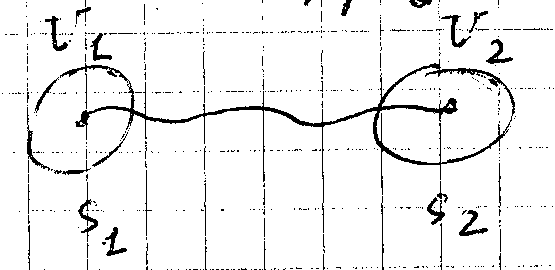
\includegraphics[width=\linewidth]{figures/gelfand-0151-p001386-path-original.png}\par\smallskip
{\footnotesize Original manuscript detail: \texttt{GELFAND-P001386}}
\end{minipage}\hfill
\begin{minipage}[t]{.50\linewidth}\vspace{0pt}\centering
{\footnotesize Partial typographic recreation}\par\smallskip
% Partial native recreation of GELFAND-P001386. No transport arrow is supplied.
% Preserve the visible break in the left oval; bottom labels remain candidates.
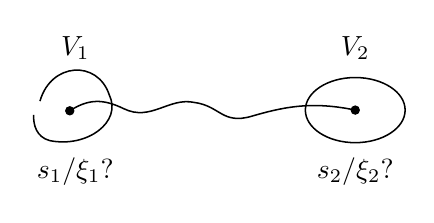
\begin{tikzpicture}[x=.88cm,y=.88cm,line width=.55pt]
\draw (-.43,.14) .. controls (-.27,.70) and (.40,.74) .. (.57,.23)
  .. controls (.76,-.16) and (.25,-.54) .. (-.29,-.43)
  .. controls (-.48,-.38) and (-.53,-.20) .. (-.52,-.06);
\draw (4.12,.01) ellipse (.72 and .47);
\draw (0,0) .. controls (.28,.18) and (.49,.17) .. (.78,.03)
  .. controls (1.17,-.16) and (1.43,.20) .. (1.80,.12)
  .. controls (2.17,.07) and (2.20,-.20) .. (2.62,-.08)
  .. controls (3.10,.06) and (3.50,.14) .. (4.12,.01);
\fill (0,0) circle (1.7pt);
\fill (4.12,.01) circle (1.7pt);
\node at (.08,.90) {$V_1$};
\node at (4.12,.90) {$V_2$};
\node at (.08,-.88) {$s_1/\xi_1$?};
\node at (4.12,-.88) {$s_2/\xi_2$?};
\end{tikzpicture}

\end{minipage}
\end{center}
\noindent{\small\textit{The left oval has a visible gap in its outline. The lower labels remain alternatives, and no direction is assigned to the wavy line. The drawing indicates the geometry only; it does not assert a transport map.}}


In locally constant sheaves one can transport sections [inserted above the line: (along a path)],
and therefore such sheaves are not \underline{flasque}.

\underline{Problem 4.}\quad $\Gamma$ is an [inserted above the line: finite] ordered set; introduce the topology
\begin{equation*}
\overline{x}:=\{y:\ y\leq x\}\quad\text{-- the closure of the point }x
\end{equation*}
a) Sheaves on $\Gamma$ $=$ representations of $\Gamma$.

b) Describe flasque sheaves on $\Gamma$.


\EnglishSourceFrame{GELFAND-P001387}{2}
c) The connection with combinatorial sheaves

Suppose that $X$ has a stratification; consider the map
\begin{tikzcd}[row sep=small]
X \arrow[d, "\pi"'] \\
\Gamma
\end{tikzcd}
(the point $x$ is sent to its stratum).

$\Gamma$ is the ordered set of strata.

[Caption beneath $\Gamma$:] Introduce the (Zariski) topology on $\Gamma$.

\underline{Assertion.}

\underline{$\forall$ combinatorial sheaves on $X$ are inverse images}
[crossed out: \EnglishUnclear{GELFAND-P001387}{cancelled-pullback}{sheaves? [source plural]}]
\underline{of sheaves on $\Gamma$}
(and conversely)
\begin{equation*}
\pi^*\colon\text{sheaves on }\Gamma\overset{\sim}{\longrightarrow}
\text{combinatorial sheaves on }X.
\end{equation*}

\underline{Exercise 5.}\quad a) Let
$0\longrightarrow\mathcal F_1\longrightarrow\mathcal F_2\longrightarrow\mathcal F_3\longrightarrow0$
be a short exact sequence of sheaves. Then the sequence of sections
\begin{equation*}
0\longrightarrow\mathcal F_1(X)\longrightarrow\mathcal F_2(X)\longrightarrow\mathcal F_3(X)
\end{equation*}
is exact.

b) If $\mathcal F_1$ is flasque, the sequence
\begin{equation*}
0\longrightarrow\mathcal F_1(X)\longrightarrow\mathcal F_2(X)\longrightarrow\mathcal F_3(X)\longrightarrow0
\end{equation*}
is exact.

\underline{A flasque resolution of a sheaf.}

\underline{Exercise 6}\quad Let $\mathcal F$ be a sheaf. Then 1) It can be embedded in
a flasque sheaf $\mathcal F\hookrightarrow G$.

2) Now construct the following exact sequence from $\mathcal F$:

\begin{center}
\begin{tikzcd}[column sep=small]
0 \arrow[r] & \mathcal F \arrow[r] & G^0 \arrow[rr] \arrow[dr] && G^1 \arrow[rr] \arrow[dr] && G^2 \arrow[r] & \ldots \\
&&& G^0/\mathcal F \arrow[ur, hook] && G^1/(G^0/\mathcal F) \arrow[ur, hook]
\end{tikzcd}
\end{center}
$G^i$ are flasque.

[Beneath the diagram:] and so on.

(a flasque resolution)

3) $\forall$ pairs of flasque resolutions can be embedded in a common third one.

\underline{Definition 3.}
\begin{equation*}
H^i(X,\mathcal F)=H^i(0\longrightarrow G^0(X)\longrightarrow G^1(X)\longrightarrow\ldots)
\end{equation*}
(Here $0\longrightarrow\mathcal F\longrightarrow G^0\longrightarrow G^1\longrightarrow\ldots$
is a flasque resolution of $\mathcal F$.)

On the right are the cohomology groups of a complex of vector spaces.

\underline{Definition 4.}\quad [Crossed out: Dual sheaf.]
\underline{Cohomology with compact support.}

Suppose that $X$ is locally compact. One can then consider
sections with compact support:
$\mathcal F_c(X)$ denotes sections with compact support on $X$.


\EnglishSourceFrame{GELFAND-P001388}{unlabelled}
\begin{equation*}
H_c^i(X,\mathcal F)=H^i(0\longrightarrow G_c^0(X)\longrightarrow G_c^1(X)\longrightarrow\ldots)
\end{equation*}

\underline{Definition 5.}\quad Dual sheaf.

Presheaf: $\mathcal F^*(V)=\mathcal F_c(V)^*$
(analogue of \EnglishUnclear{GELFAND-P001388}{dual-note}{distributions? [source genitive plural] / a distribution? [source singular ending]})

(the dual space in the sense of linear algebra)
\begin{equation*}
V_1\subset V_2\ \Rightarrow\ \mathcal F_c(V_1)\longrightarrow\mathcal F_c(V_2)
\quad\text{(inclusion)}
\end{equation*}
and $\mathcal F^*(V_2)\longrightarrow\mathcal F^*(V_1)$ arises.

\underline{Exercise 7.}

a) $\mathcal F^*$ is a sheaf if $\mathcal F$ is flasque.

b) If $\mathcal F^*$ is a sheaf, then $\mathcal F^*$ is flasque, i.e.
$\forall\underset{\text{open}}{V}\subset X$,
the map $\mathcal F^*(X)\longrightarrow\mathcal F^*(V)$ is surjective.


\EnglishSourceFrame{GELFAND-P001389}{unlabelled}
\underline{12.10.87.}\qquad \underline{Gelfand seminar.}

Vakhtangov told the actors in Princess Turandot to enter the stage in fashionable clothes
and change immediately (putting on a turban and so on). The stories of mathematics are eternal; only the language changes.

\underline{I. M. G.}\quad
\underline{On a combinatorial conjecture of Dyson concerning multinomial coefficients}

\underline{A paper from the thick green collection on combinatorics}

Consider
\begin{equation*}
F(x,a)=\prod_{i\neq j}\left(1-\frac{x_j}{x_i}\right)^{a_j},
\qquad a_j\in\mathbb N.\tag{1}
\end{equation*}
Find the constant term.

Dyson's conjecture (1962): the answer is
\begin{equation*}
\frac{(a_1+a_2\ldots+a_n)!}{a_1!a_2!\ldots a_n!}\tag{2}
\end{equation*}

In 1962, two (long) proofs were given in J. Math. Phys.

In 1970, a two-line proof in J. Math. Phys. by \EnglishUnclear{GELFAND-P001389}{author-name}{Wood? / Good? [source candidates: «Вуда» / «Гуда»]}.

\underline{Proof.}\quad Applying Lagrange's interpolation formula to the function
\EnglishUnclear{GELFAND-P001389}{interpolation-function}{$f\equiv0$}
and then setting $x=0$, we obtain
\begin{equation*}
\sum_j\prod_{i\neq j}\left(1-\frac{x_j}{x_i}\right)^{-1}=1\tag{3}
\end{equation*}

Multiplying by $F(x,a)$, we obtain


\EnglishSourceFrame{GELFAND-P001390}{unlabelled}
\begin{equation*}
\sum_j F(x,a_1,\ldots,a_{j-1},a_j-1,a_{j+1},\ldots,a_n)=F(x,a)\tag{4}
\end{equation*}

[Crossed out: \EnglishUnclear{GELFAND-P001390}{cancelled-let}{an illegible beginning.}]
Let $G(a)$ be the constant term. Then, from (4),
\begin{equation*}
G(a)=\sum G(a_1,\ldots,a_{j-1},a_j-1,a_{j+1},\ldots,a_n),\tag{5}
\end{equation*}
which gives a recurrence formula.

For $a_j=0$, we obtain
\begin{equation*}
G(a_1,\ldots,a_{j-1},0,a_{j+1},\ldots,a_n)
=G(a_1,\ldots,a_{j-1},a_{j+1},\ldots,a_n)\tag{6}
\end{equation*}
In addition,
\begin{equation*}
G(0)=1\tag{7}
\end{equation*}
Relations (5)--(7) are sufficient recurrence relations
to determine everything, and we obtain (2).

\underline{A. Veselov}

\underline{On geodesics on an ellipsoid and motion on a sphere}

Following Jacobi and others---1982: Kn\"orrer's observation, the equivalence of two problems.

[Two columns follow, separated by a brace-shaped line. Left column.]

1) $(Aq,q)=1$

Geodesics on an ellipsoid

Weierstrass found them in $\theta$-functions (1861).

The geodesic equation in the natural parameter:
\begin{equation*}
\ddot q=\lambda Aq\tag{1}
\end{equation*}
(acceleration $\sim$ the normal)

[Addition on the right, in parentheses:]
$\lambda$ is the Lagrange multiplier, found from the condition $(Aq,q)=1$.

[Right column.]

2) Another problem [crossed out: \EnglishUnclear{GELFAND-P001390}{cancelled-neumann}{C. Neu...?}]
C. Neumann (1859)

Motion with potential energy
\begin{equation*}
U(x)=\frac12(Ax,x)
\end{equation*}
on the sphere $|x|^2=1$.

Here the equation is
\begin{equation*}
x''=-Ax+ux\tag{$1'$}
\end{equation*}
or, in coordinates,
\begin{equation*}
x_i''=-a_i x_i+ux_i\tag{$1''$}
\end{equation*}
[On the right, a sign is crossed out: \EnglishUnclear{GELFAND-P001390}{equation-end}{$q$? / $u$?}]

[Continuation below the columns.]

Pass to another parameter:
\begin{equation*}
q''=-Aq+vq'\tag{2}
\end{equation*}
(the substitutions are written out explicitly, $\lambda\rightsquigarrow v$).

\EnglishUnclear{GELFAND-P001390}{constants-note}{Beneath $\lambda$ and $v$ are two short vertical strokes each, with const written beneath each pair.}

Then the substitution
\begin{equation*}
x=\frac{Aq}{|Aq|}\qquad\text{(Gauss substitution)}\tag{3}
\end{equation*}
takes solutions of problem 1) to solutions of problem 2)
(and \EnglishUnclear{GELFAND-P001390}{bijection-note}{vzaimoodn.? [unexpanded source abbreviation: «взаимоодн.»]}).

(H. Kn\"orrer, 1982)

Equation

[On the right:] Introduce an operator:
\begin{equation*}
L=-\frac{d^2}{dt^2}+u,\qquad Lx_i=a_i x_i\tag{4}
\end{equation*}
($x_i$ is an eigenfunction!!)


\EnglishSourceFrame{GELFAND-P001391}{12}
On the left:
\begin{equation*}
\widetilde L=-\frac{d^2}{dt^2}+v\frac{d}{dt}\tag{5}
\end{equation*}
(conjugate to $L$ by the Gauss substitution or the Miura substitution)

Kn\"orrer arrived at this through the Moser--Trubowitz isomorphism.

\underline{Consider problem 2).}

There are two symplectic forms.

\underline{Problem (I. M. G.)}\quad Given a symmetric matrix $A$ and a rank-one matrix $K$,
From the eigenvalues of $A+K$, how can one recover $K$? ($A$ is fixed.)

This is precisely Jacobi's formula.

\underline{V.}\quad For $n=2$, introduce new coordinates:
\begin{gather*}
M=[\dot x,x],\qquad\text{(angular momentum---cross product)}\\
p=x
\end{gather*}

$1^{\circ}$. The Lie--Berezin--Kirillov bracket
\begin{gather*}
\{M_i,M_j\}=\varepsilon_{ijk}M_k\\
\{M_i,p_j\}=\varepsilon_{ijk}p_k\\
\{p_i,p_j\}=0
\end{gather*}
The Hamiltonian
\begin{equation*}
2H=M^2+(Ap,p)
\end{equation*}
Then
\begin{equation*}
\begin{cases}
\dot M_i=\{M_i,H\}\\
\dot p_i=\{p_i,H\}
\end{cases}
\qquad\text{-- Neumann's equations}
\end{equation*}

\underline{Second bracket}
\begin{gather*}
\varepsilon_{ijk}a_kM_k=\{M_i,M_j\}\\
\varepsilon_{ijk}a_kp_k=\{M_i,p_j\}\\
\varepsilon_{ijk}M_k=\{p_i,p_j\}
\end{gather*}
The Hamiltonian $F=\frac12p^2$

\underline{I. M. G.}\quad This coincides with what Arnold described

(see the previous notebook).

The system is Hamiltonian with respect to both.


\EnglishSourceFrame{GELFAND-P001392}{unlabelled}
\underline{A. Beilinson.}\quad \underline{Constructible sheaves} (continued)

Representations of a partially ordered set $\Longleftrightarrow$
[crossed out: \EnglishUnclear{GELFAND-P001392}{cancelled-equivalence}{constructible?}]
combinatorial sheaves

\begin{center}
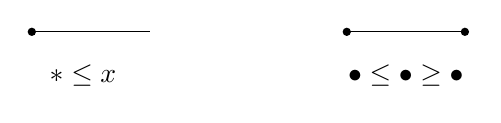
\begin{tikzpicture}
\draw (0,0) -- (1.5,0);
\fill (0,0) circle (1.5pt);
\node at (0.65,-0.55) {$\ast\leq x$};
\draw (4,0) -- (5.5,0);
\fill (4,0) circle (1.5pt);
\fill (5.5,0) circle (1.5pt);
\node at (4.75,-0.55) {$\bullet\leq\bullet\geq\bullet$};
\end{tikzpicture}
\end{center}

A combinatorial sheaf is a sheaf constant on each stratum.

\underline{Homological algebra.}

$\mathcal A$ is an abelian category (for example, sheaves over a given space or modules).

$C(\mathcal A)$ is the category of complexes over $\mathcal A$.

One needs to know the \underline{derived category} (Verdier, 1961).

Objects \EnglishUnclear{GELFAND-P001392}{objects-mark}{crossed-out ``from''? / a membership sign?}
$C(\mathcal A)$
\begin{gather*}
\ldots\longrightarrow X^i\overset{d}{\longrightarrow}X^{i+1}
\overset{d}{\longrightarrow}X^{i+2}\longrightarrow\ldots\\
d^2=0
\end{gather*}
Morphisms are morphisms of complexes (families of morphisms
\begin{tikzcd}[row sep=small]
X^i \arrow[d, "\varphi"'] \\
Y^i
\end{tikzcd} commuting with $d$).

$C(\mathcal A)$ is also an abelian category.

Bounded complexes (only finitely many terms $\neq0$): $C^b(\mathcal A)$

Bounded on the left or on the right: $C^{\pm}(\mathcal A)$
\begin{gather*}
C^+(\mathcal A)\text{ -- bounded on the left}\\
C^-(\mathcal A)\text{ -- bounded on the right}
\end{gather*}

The homotopy category $K(\mathcal A)$

The objects of $K(\mathcal A)$ are the same as those of $C(\mathcal A)$, and the morphisms are equivalence classes
of morphisms of $C(\mathcal A)$ under homotopy.
\begin{equation*}
\operatorname{Hom}_{K(\mathcal A)}(X^\bullet,Y^\bullet)
\end{equation*}

A morphism $X^\bullet\overset{\varphi}{\longrightarrow}Y^\bullet$ is [inserted above the line: such]
a family $\varphi^i\colon X^i\longrightarrow Y^i$ that the diagram commutes:

\par\noindent\begin{minipage}{\linewidth}\vspace{0pt}
[On the left:]
\par\nopagebreak[4]
\begin{center}
\begin{tikzcd}
X^{i-1} \arrow[r, "d"] \arrow[d, "{\varphi^{i-1}}"'] &
X^i \arrow[r, "d"] \arrow[d, "{\varphi^i}"] \arrow[dl, dashed, "{\psi^i}"'] &
X^{i+1} \arrow[d, "{\varphi^{i+1}}"] \arrow[dl, dashed, "{\psi^{i+1}}"'] \\
Y^{i-1} \arrow[r, "d"] & Y^i \arrow[r, "d"] & Y^{i+1}
\end{tikzcd}
\end{center}
\end{minipage}\par
\par\noindent\begin{minipage}{\linewidth}\vspace{0pt}
[On the right:]
\par\nopagebreak[4]
\begin{center}
\begin{tikzcd}
X^i \arrow[r, "d"] \arrow[d, "{\varphi^i}"'] & X^{i+1} \arrow[d, "{\varphi^{i+1}}"] \\
Y^i \arrow[r, "d"] & Y^{i+1}
\end{tikzcd}
\end{center}
\end{minipage}\par
[A wavy line goes around the left diagram above and on the right, then passes beneath the right diagram.]

$\varphi$ is called \underline{null-homotopic} if $\exists$ a family of maps
$X^i\overset{\psi^i}{\longrightarrow}Y^{i-1}$
such that
\begin{equation*}
\varphi^i=d\psi^i+\psi^{i+1}d\tag{1}
\end{equation*}


\EnglishSourceFrame{GELFAND-P001393}{13}
\underline{Exercise 1.}\quad Check that, for any family of maps $\psi^i$, the family (1)
defines a morphism of complexes, i.e. $d\varphi_i=\varphi_{i+1}d$.

\underline{Exercise 2.}\quad Morphisms homotopic to $0$ form an ideal, i.e. if
$\varphi$ is homotopic to $0$ and $\varphi_1$ is any morphism, then
$\varphi\circ\varphi_1$ is homotopic to $0$.

(The same is true for the composition $\varphi_2\circ\varphi$ with any morphism $\varphi_2$.)
\begin{equation*}
\operatorname{Hom}_{K(\mathcal A)}(X^\bullet,Y^\bullet)
=\operatorname{Hom}_{C(\mathcal A)}(X^\bullet,Y^\bullet)
/\bigl(\text{morphisms homotopic to }0\bigr)
\end{equation*}
There are obvious functors
\begin{equation*}
\mathcal A\longrightarrow C(\mathcal A)\longrightarrow K(\mathcal A)
\end{equation*}
The cohomology functor
\begin{equation*}
H^i\colon C(\mathcal A)\longrightarrow\mathcal A\qquad
\left(H^i(X^\bullet)=
\frac{\ker(d\colon X^i\longrightarrow X^{i+1})}
{\operatorname{Im}(d\colon X^{i-1}\longrightarrow X^i)}\right)
\end{equation*}

\underline{Exercise 3.}\quad Prove that $\exists!$ a functor
$H^i\colon K(\mathcal A)\longrightarrow\mathcal A$ such that
\begin{center}
\begin{tikzcd}
C(\mathcal A) \arrow[r] \arrow[dr, "{H^i}"'] & K(\mathcal A) \arrow[d, "{H^i}"] \\
& \mathcal A
\end{tikzcd}
\end{center}
The action of $H^i$ on morphisms is also defined in the obvious way.

\underline{Definition.}\quad $\varphi\colon X^\bullet\longrightarrow Y^\bullet$
[beneath the arrow: in the category $K(\mathcal A)$]
is called a \underline{quasi-isomorphism} if it induces an isomorphism
\begin{equation*}
H^i(X^\bullet)\longrightarrow H^i(Y^\bullet).
\end{equation*}

\underline{The derived category.}

\underline{Exercise 4.}\quad Suppose that there are three complexes
\begin{center}
\begin{tikzcd}
X^\bullet & & Y^\bullet \\
& Z^\bullet \arrow[ul, "\alpha"] \arrow[ur, "\beta"'] &
\end{tikzcd}
\end{center}
and morphisms, with $\alpha$ a quasi-isomorphism.

Then there exists a (commutative) diagram
\begin{center}
\begin{tikzcd}
& Z' & \\
X^\bullet \arrow[ur, "{\alpha'}"] & & Y^\bullet \arrow[ul, "{\beta'}"'] \\
& Z^\bullet \arrow[ul, "\alpha"] \arrow[ur, "\beta"'] &
\end{tikzcd}
\end{center}
[To the left of the lower part of the diagram, crossed out:
\EnglishUnclear{GELFAND-P001393}{cancelled-left}{in which? [abbreviated in the source]}.]

in which $\beta'$ is a quasi-isomorphism.

The same holds if one starts from the diagram
\begin{center}
\begin{tikzcd}
& Z' & \\
X^\bullet \arrow[ur, "{\alpha'}"] & & Y^\bullet \arrow[ul, "{\beta'}"']
\end{tikzcd}
\end{center}
with the quasi-isomorphism $\alpha'$.


\EnglishSourceFrame{GELFAND-P001394}{unlabelled}
\underline{The derived category} $D(\mathcal A)$

Objects $=$ the objects of $K(\mathcal A)$ (i.e. complexes)

Morphisms [inserted above the line: $X^\bullet\longrightarrow Y^\bullet$] are equivalence classes of diagrams
\begin{center}
\begin{tikzcd}
X^\bullet & & Y^\bullet \\
& Z^\bullet \arrow[ul, "\alpha"] \arrow[ur, "\beta"'] &
\end{tikzcd}
\qquad $\beta\alpha^{-1}$
\end{center}
($\alpha$ is a quasi-isomorphism)

under the equivalence relation \underline{generated}
by the \EnglishUnclear{GELFAND-P001394}{elementary-abbrev}{elm.? / elem.? [unexpanded source abbreviations]} relation.

[Crossed out: \EnglishUnclear{GELFAND-P001394}{cancelled-there}{There is? / If?}.]

(There is a functor $K(\mathcal A)\longrightarrow D(\mathcal A)$.)

\begin{center}
\begin{tikzcd}
X^\bullet & & Y^\bullet \\
& Z^\bullet \arrow[ul, "\alpha"] \arrow[ur, "\beta"'] & \\
& T \arrow[u, "\gamma"] &
\end{tikzcd}
\end{center}

\EnglishUnclear{GELFAND-P001394}{fraction-relation}{$\beta\alpha^{-1}\sim\beta\gamma(\alpha\gamma)^{-1}$?},
where $\gamma$ is a quasi-isomorphism.

\begin{center}
\begin{tikzcd}
X^\bullet & & Y^\bullet \\
& Z^\bullet \arrow[ul, "\alpha"] \arrow[ur, "\beta"'] &
\end{tikzcd}
\quad $\sim$ \quad
\begin{tikzcd}
X^\bullet & & Y^\bullet \\
& T \arrow[ul, "{\alpha\gamma}"] \arrow[ur, "{\beta\gamma}"'] &
\end{tikzcd}
\end{center}

These morphisms can now be composed.

\begin{center}
\begin{tikzcd}
X^\bullet & & Y^\bullet & & W \\
& Z^\bullet \arrow[ul] \arrow[ur] & & T \arrow[ul] \arrow[ur] & \\
& & S \arrow[ul] \arrow[ur] & &
\end{tikzcd}
\end{center}
[To the right of the lower part of the diagram, a left-pointing arrow with the caption:]
$\longleftarrow$ complete it \underline{by the lemma}.

The composition is the outer side of the diagram.

\EnglishSourceFrame{GELFAND-P001395}{unlabelled}
\underline{19.10.87.}\quad \underline{Gelfand seminar.}

\underline{I. M. Gelfand}\quad
\underline{Calculating sums of $k$th powers and other sums}

\EnglishUnclear{GELFAND-P001395}{speaker-parenthesis}{(following a recent thought) / (following an unclear thought)}

\begin{equation*}
F'(x)=f(x)\qquad f(x)=x^k;\qquad F(x)=\frac{x^{k+1}}{k+1}
\end{equation*}
\begin{align*}
F(2)-F(1)&=\frac{f(1)}{1!}+\frac{f'(1)}{2!}+\frac{f''(1)}{3!}+\ldots\\
F(3)-F(2)&=\frac{f(2)}{1!}+\frac{f'(2)}{2!}+\frac{f''(2)}{3!}+\ldots\\[8pt]
F(n+1)-F(n)&=f(n)+\frac{f'(n)}{2!}+\frac{f''(n)}{3!}+\ldots
\end{align*}
\rule{9cm}{0.3pt}
\begin{equation*}
F(n+1)-F(1)=S_0+\frac{S_1}{2!}+\frac{S_2}{3!}+\ldots
\end{equation*}
Similarly,
\begin{align*}
f(n+1)-f(1)&=S_1+\frac{S_2}{2!}+\ldots\\
f'(n+1)-f'(1)&=S_2+\frac{S_3}{2!}+\ldots\\
\ldots\qquad&\ldots\\
f^{(p)}(n+1)-f^{(p)}(1)&=\ldots\quad
\EnglishUnclear{GELFAND-P001395}{system-last-index}{S_p}+\ldots
\end{align*}

[To the right of the system:]
Here
\begin{align*}
S_0&=f(1)+f(2)+\ldots+f(n)\\
S_1&=f'(1)+f'(2)+\ldots+f'(n)\\
&\ldots\\
S_k&=f^{(k)}(1)+f^{(k)}(2)+\ldots+f^{(k)}(n)
\end{align*}

Hence
[to the left of the determinant, crossed out:
\EnglishUnclear{GELFAND-P001395}{determinant-cancellation}{det / illegible}]
\begin{equation*}
S_0=\frac{
\begin{vmatrix}
F(n+1)-F(1)&\dfrac{1}{2!}&\dfrac{1}{3!}&\ldots\\
f(n+1)-f(1)&1&\dfrac{1}{2!}&\\
f'(n+1)-f'(1)&0&1&\\
\ldots&0&0&
\end{vmatrix}}{1}
\end{equation*}

Expand along the first column:
\begin{equation*}
S_0=A_0\bigl(F(n+1)-F(1)\bigr)
+A_1\bigl(f(n+1)-f(1)\bigr)+\ldots
\end{equation*}
The coefficients are universal---valid for $\forall$ functions!!

Substitute $f(x)=e^{tx}$.

Banded determinants arise!

[Crossed out:
\EnglishUnclear{GELFAND-P001395}{exponential-cancellation}{$S_0=A_0$ / illegible}]
\begin{equation*}
\EnglishUnclear{GELFAND-P001395}{exponential-fraction}{\frac{\dfrac{1}{n+1}e^{t(n+1)}-e}{e^t-1}}
\end{equation*}
Expand [crossed out:
\EnglishUnclear{GELFAND-P001395}{series-cancellation}{series / illegible}]
in $t$\quad $\Longrightarrow$ \underline{Bernoulli numbers}.

\underline{Problem.} The symmetric group $S_n$
\EnglishUnclear{GELFAND-P001395}{symmetric-group-predicate}{is generated / is defined}
[inserted above the line: ``(\EnglishUnclear{GELFAND-P001395}{group-generator-abbreviation}{obrts. / obr. [unexpanded source abbreviations]} $s_1,\ldots,s_{n-1}$)'']
by the relations
\begin{equation*}
s_i^2=1,\qquad s_i s_j=s_j s_i\quad\text{for }|i-j|\ge2,
\qquad (s_i s_{i+1})^3=1
\end{equation*}
Consider a parabolic subgroup:
\begin{equation*}
G=\Sigma_n,\qquad H=\Sigma_k\times\Sigma_{n-k},\qquad G\supset H
\end{equation*}
\begin{equation*}
\mathcal A=\mathbb C[G]=
\left\{\sum_{g\in G}a_g g,\quad a_g\in\mathbb C\right\}
\end{equation*}


\EnglishSourceFrame{GELFAND-P001396}{23}
\begin{equation*}
\mathcal A\supset
\underset{\text{subalgebra}}{\mathcal A'}
=\{x\in A,\ xh=hx=x\text{ for every }h\in H\}
\end{equation*}

[Crossed-out sign before the heading:
\EnglishUnclear{GELFAND-P001396}{heading-cancellation}{illegible}]
\underline{Beilinson A.}\quad (continued)

\underline{Derived categories}

\begin{tikzcd}[row sep=small,column sep=small]
\mathcal A\arrow[d]&\text{--- an abelian category}\\
C(\mathcal A)\arrow[d]&\text{--- the category of complexes over }\mathcal A\\
K(\mathcal A)\arrow[d]&\text{--- the homotopy category}\\
D(\mathcal A)&\text{--- the derived category}
\end{tikzcd}

The objects of $D(\mathcal A)$ are complexes; the morphisms are equivalence classes of diagrams.

\EnglishSourceFigure{GELFAND-P001396}{roof-cancellation}{A crossed-out diagram: $X$ above on the left, $Y$ above on the right, $Z$ below between them; slanting strokes from the lower node towards the upper ones and a broad repeated zigzag cancellation are visible. The exact arrow strokes beneath the cancellation cannot be established.}

\begin{center}
\begin{minipage}[t]{.46\linewidth}\vspace{0pt}\centering
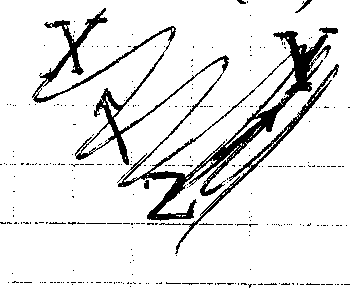
\includegraphics[width=\linewidth]{figures/gelfand-0152-p001396-roof-original-r2.png}\par\smallskip
{\footnotesize Original manuscript detail: \texttt{GELFAND-P001396}}
\end{minipage}\hfill
\begin{minipage}[t]{.50\linewidth}\vspace{0pt}\centering
{\footnotesize Partial visible-stroke recreation}\par\smallskip
% Partial visible-stroke recreation. No hidden morphism direction is supplied.
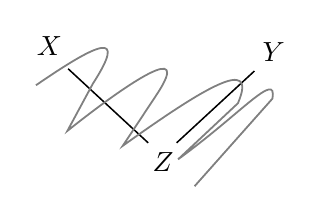
\begin{tikzpicture}[x=.95cm,y=.95cm,line width=.55pt]
\node at (0,1.25) {$X$};
\node at (3,1.18) {$Y$};
\node at (1.52,-.3) {$Z$};
\draw (.25,.95)--(1.32,-.04);
\draw (1.7,-.04)--(2.74,.92);
\draw[gray,line width=.65pt] (-.18,.73)
  .. controls (.65,1.3) and (1.05,1.48) .. (.58,.75)
  --(.24,.12) .. controls (1.12,.82) and (1.88,1.3) .. (1.45,.63)
  --(.98,-.08) .. controls (2.03,.67) and (2.8,1.15) .. (2.52,.49)
  --(1.72,-.26) .. controls (2.56,.35) and (3.05,.94) .. (2.98,.55)
  --(1.94,-.62);
\end{tikzpicture}

\end{minipage}
\end{center}
\noindent{\small\textit{The cancelled nodes are readable, but the directions beneath cancellation are not recovered. Plain connecting strokes do not assert morphisms.}}


\begin{tikzcd}[row sep=small,column sep=small]
&Z'&\\
X\arrow[ur]&&Y\arrow[ul,shorten <=8pt,shorten >=8pt]\\
&Z\arrow[ul,shorten <=8pt,shorten >=8pt]\arrow[ur]&
\end{tikzcd}
\quad (quasi-isomorphisms are shorter).

\underline{Example 1.} Let $X$ be a complex with
[crossed out: \EnglishUnclear{GELFAND-P001396}{example-cancellation}{so [unresolved source fragment] / illegible}]
$H^i(X)=0$ for $i\ne0$.
Then $X$ is canonically quasi-isomorphic to $H^0(X)$:
\begin{equation*}
X\cong H^0(X)\text{ in }D(\mathcal A)
\end{equation*}
(This is not so in the homotopy category!)

For the complex $X$, introduce the subcomplex $\tau_{\le0}(X)$ in $X$:
\begin{equation*}
\text{(1)}\qquad
\tau_{\le0}(X)^i=
\begin{cases}
X^i,&i<0\\
\ker d:X^0\to X^1,&i=0\\
0,&i>0
\end{cases}
\end{equation*}
It is easy to see that
\begin{equation*}
\text{(2)}\qquad
H^j(\tau_{\le0}(X))=
\begin{cases}
H^j(X),&j\le0\\
0,&j>0
\end{cases}
\end{equation*}
The diagram

(3)
\EnglishSourceFigure{GELFAND-P001396}{truncation-diagram}{At the bottom is $\tau_{\le0}(X)$; arrows go from it upwards to the left towards $X$ and upwards to the right towards $H^0(X)$. The right arrow has $\sim$. Beside the left arrow is a sign resembling a rotated tilde, $2$ or $\iota$; below on the left is the caption ``canonical inclusion''. To the right of the diagram is a separate short hook-shaped stroke.}

\def\GelfandCanonicalInclusionCaption{canonical\\inclusion}
\begin{center}
\begin{minipage}[t]{.46\linewidth}\vspace{0pt}\centering
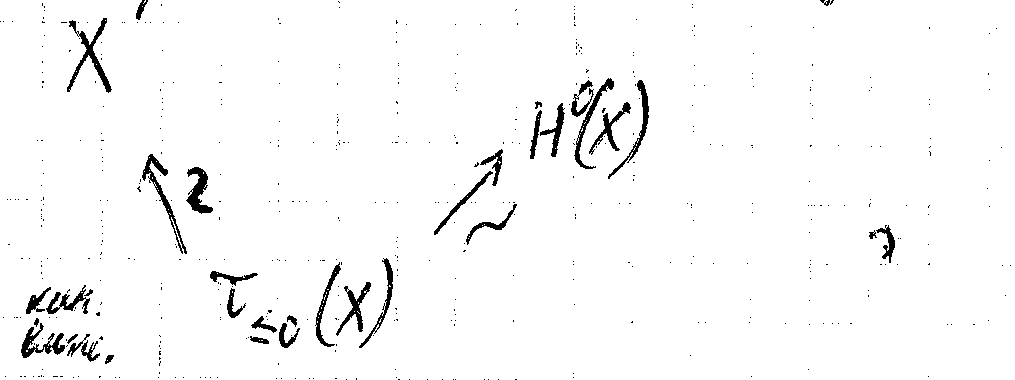
\includegraphics[width=\linewidth]{figures/gelfand-0152-p001396-truncation-original-r2.png}\par\smallskip
{\footnotesize Original manuscript detail: \texttt{GELFAND-P001396}}
\end{minipage}\hfill
\begin{minipage}[t]{.50\linewidth}\vspace{0pt}\centering
{\footnotesize Partial visible-stroke recreation}\par\smallskip
% Requires the language-local caption macro \GelfandCanonicalInclusionCaption.
% The label on the left remains a candidate list, not a selected reading.
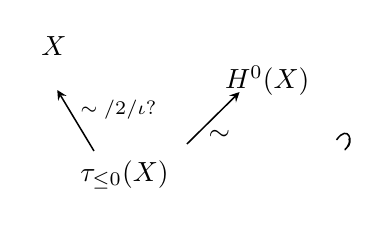
\begin{tikzpicture}[x=.88cm,y=.88cm,line width=.55pt,>=stealth]
\node at (0,1.55) {$X$};
\node at (3.08,1.05) {$H^0(X)$};
\node at (1.02,-.30) {$\tau_{\le0}(X)$};
\draw[->] (.58,.04)--(.05,.92);
\draw[->] (1.92,.14)--(2.68,.89);
\node[font=\scriptsize] at (.93,.64) {$\sim/2/\iota$?};
\node at (2.39,.26) {$\sim$};
\node[anchor=east,font=\scriptsize,align=right] at (-.10,-.33) {\GelfandCanonicalInclusionCaption};
% The isolated right-hand ink stroke has no assigned mathematical meaning.
\draw (4.08,.20) .. controls (4.25,.44) and (4.34,.16) .. (4.22,.08)
  .. controls (4.16,.02) and (4.30,.13) .. (4.26,.22);
\end{tikzpicture}

\end{minipage}
\end{center}
\noindent{\small\textit{The left arrow label remains tilde/2/iota candidates. Its being a quasi-isomorphism in this example does not settle the written sign. The isolated right stroke is retained without interpretation.}}


defines the required isomorphism in $D(\mathcal A)$.

[Crossed out:
\EnglishUnclear{GELFAND-P001396}{cancelled-bottom-sentence}{This same complex could have been looked at}]

\underline{Remark.} A complex $X$ with several non-$0$ groups $H^i$
is \underline{not} quasi-isomorphic (in general) to their sum, and if
[inserted above the line: ``(quasi)''] it is, then not uniquely.


\EnglishSourceFrame{GELFAND-P001397}{unlabelled}
\underline{The structure of a triangulated category}

$K(A)$ and $D(A)$ are not abelian categories.

\underline{Exercise 1.} Check that
$K(A)$ is abelian $\Longleftrightarrow\mathcal A$ is semisimple

($\mathcal A$ is semisimple $\Longleftrightarrow$
$[(\forall\text{ object})=(\text{a direct sum of irreducibles})]$).

\underline{The cone of a morphism.}

Let $f:X\longrightarrow Y$\quad be a morphism of complexes.

\begin{tikzcd}[row sep=small,column sep=large]
X^1\arrow[r,"f^1"]\arrow[dr,dashed,no head]&Y^1\\
X^0\arrow[u]\arrow[r,"f^0"]\arrow[dr,dashed,no head]&Y^0\arrow[u]\\
X^{-1}\arrow[u]\arrow[r,"f^{-1}"]&Y^{-1}\arrow[u]
\end{tikzcd}

Consider all of this as a bicomplex, i.e.
write the complex
\begin{equation*}
C(f)^i=\EnglishUnclear{GELFAND-P001397}{cone-coordinate-order}{Y^i\oplus X^{i+1}}
\end{equation*}
\begin{equation*}
d(x,y)=(-d(x),d(y)+f(x))
\end{equation*}

There is a sequence
\begin{equation*}
\text{(4)}\qquad
C(f[-1])\longrightarrow X\overset{f}{\longrightarrow}Y
\underset{g}{\longrightarrow}C(f)\longrightarrow X[1]\longrightarrow
\end{equation*}
[Above the arrow $Y\to C(f)$, crossed out:
\EnglishUnclear{GELFAND-P001397}{sequence-arrow-cancellation}{illegible};
beneath $g$: ``inclusion''.]
[Before $C(f)$, crossed out:
\EnglishUnclear{GELFAND-P001397}{sequence-object-cancellation}{$X$ / $Y$}.]
[Beneath $X[1]$: ``a shift of the grading and a change of sign of $d$''.]
\begin{equation*}
\longrightarrow Y(1)\longrightarrow
\EnglishUnclear{GELFAND-P001397}{sequence-shifted-cone}{C(f[1])\text{ / }C(f)[1]}
\longrightarrow X[2]\longrightarrow
\end{equation*}
[Between $X$ and $[2]$, crossed out:
\EnglishUnclear{GELFAND-P001397}{sequence-shift-cancellation}{( / [1] / illegible}.]

It goes into itself under a shift of three steps.
In the homotopy category it goes into itself under a shift of one step.

\begin{equation*}
\text{(5)}\qquad Y\overset{g}{\longrightarrow}C(f)\longrightarrow C(g)
\end{equation*}
(6) \underline{Assertion.} In $K(A)$, the complex $C(g)=X[1]$.

There is a map:
\begin{tikzcd}[row sep=small,column sep=large]
Y\arrow[r]\arrow[d,equal]&C(f)\arrow[r]\arrow[d,equal]&X[1]\\
Y\arrow[r]&C(f)\arrow[r]&C(g)\arrow[u]
\end{tikzcd}

Namely,
\begin{equation*}
C(g)^i=C(f)^i\oplus Y^{i+1}=X^{i+1}\oplus Y^i\oplus Y^{i+1}
\end{equation*}
projects onto $X^{i+1}$.


\EnglishSourceFrame{GELFAND-P001398}{24}
\underline{Exercise 2}. Check that this is a morphism of complexes and
an isomorphism in the homotopy category.

\underline{Exercise 3}. In $K(A)$, find the cones $C(id)$ and $C(0)$.
[Beneath $id$: identity map; beneath $0$: zero map.]

\underline{Definition 1}. A triangle in $K(A)$ or $D(A)$ is
a diagram
\begin{center}
\begin{tikzcd}[column sep=small]
\cdots \arrow[r] & Z[-1] \arrow[r,"{\gamma[-1]}"] & X \arrow[r,"\alpha"] &
Y \arrow[r,"\beta"] & Z \arrow[r,"\gamma"] & X[1] \arrow[r,"{\alpha[1]}"] &
Y[1] \arrow[r,"{\beta[1]}"] & Z[1] \arrow[r,"{\gamma[1]}"] & \cdots
\end{tikzcd}
\end{center}

[Crossed out: \EnglishSourceFigure{GELFAND-P001398}{cancelled-sketch}{A sketch beneath the diagram: on the left, an almost vertical stroke with its end pointing upwards; on the right, a slanting stroke with its end pointing upwards to the right. Several slanting cancellation lines pass between and over them. Possible letter labels beneath the cancellation cannot be distinguished confidently.}]

\begin{center}
\begin{minipage}[t]{.46\linewidth}\vspace{0pt}\centering
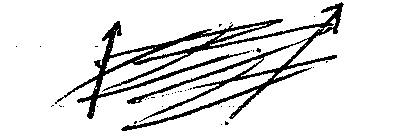
\includegraphics[width=\linewidth]{figures/gelfand-0152-p001398-cancelled-sketch-original-r2.png}\par\smallskip
{\footnotesize Original manuscript detail: \texttt{GELFAND-P001398}}
\end{minipage}\hfill
\begin{minipage}[t]{.50\linewidth}\vspace{0pt}\centering
{\footnotesize Partial visible-stroke recreation}\par\smallskip
% Visible pointed strokes and cancellation only; no node labels are recovered.
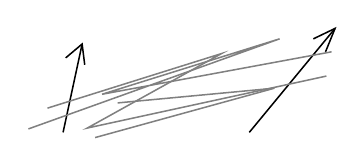
\begin{tikzpicture}[x=1.10cm,y=1.10cm,line width=.55pt]
\draw (0,0)--(.22,1.02);
\draw (.03,.86)--(.22,1.02)--(.25,.78);
\draw (2.15,0)--(3.14,1.20);
\draw (2.89,1.08)--(3.14,1.20)--(3.03,.93);
\draw[gray] (-.40,.04)--(2.50,1.08)--(.45,.44)--(3.1,.93);
\draw[gray] (-.18,.28)--(1.83,.91)--(.28,.05)--(3.04,.65);
\draw[gray] (.37,-.06)--(2.44,.51)--(.63,.34);
\end{tikzpicture}

\end{minipage}
\end{center}
\noindent{\small\textit{Only the visible pointed strokes and cancellation are recreated. No hidden node letters, arrow labels or connections are supplied.}}


\underline{\underline{Definition 2}}. An exact triangle in $K(A)$ or $D(A)$ is
a triangle isomorphic to the triangle:
\begin{center}
\begin{tikzcd}[column sep=small]
{} \arrow[r] & X \arrow[r,"f"] & Y \arrow[r,"g"] & C(f) \arrow[r] &
X[1] \arrow[r] & Y[1] \arrow[r] & \cdots
\end{tikzcd}
\end{center}


\EnglishSourceFrame{GELFAND-P001399}{unlabelled}
\underline{9/XI-87.}\qquad \underline{\underline{Gelfand seminar}}

[Crossed out: Lascoux.]\qquad \underline{Lascoux}

\underline{I. M. G. following Lascoux}
(\EnglishUnclear{GELFAND-P001399}{heading-parenthesis}{beautiful / correct} series)

Schubert polynomials.

Consider the polynomial
\begin{equation*}
P=\alpha u+\beta\EnglishUnclear{GELFAND-P001399}{equation-1-second-variable}{u\text{ or }v}+\gamma w+\cdots \tag{1}
\end{equation*}
$u,v,w$ [crossed out: \EnglishUnclear{GELFAND-P001399}{cancelled-coefficients}{$\alpha,\beta,\gamma$}] are monomials.

In our case, we will have $u,v,w,$ [one sign crossed out:
\EnglishUnclear{GELFAND-P001399}{cancelled-after-w}{illegible}] $\ldots=x_1,x_2,\ldots,x_n$.

$\alpha,\beta,\gamma,\ldots$ are numbers.

The polynomials [crossed out: \EnglishUnclear{GELFAND-P001399}{cancelled-before-sm}{function / functions [source abbreviations]}]
$S^m(P)$ [crossed out: \EnglishUnclear{GELFAND-P001399}{cancelled-after-sm}{Schur}]
are defined by the formula
\begin{equation*}
\sum_{\EnglishUnclear{GELFAND-P001399}{equation-2-lower-bound}{m\ge0\text{ or }m=0}}^{\infty}
z^m S^m(P)=\frac{1}{(1-zu)^\alpha(1-zv)^\beta\ldots} \tag{2}
\end{equation*}
\begin{equation*}
\alpha=\beta=\gamma=\cdots=1\quad\Rightarrow
\end{equation*}
\begin{equation*}
S^m(x_1+x_2+\cdots+x_n)=\sum_{i_1\le i_2\le\cdots\le i_m}
x_{i_1}x_{i_2}\cdots x_{i_m} \tag{3}
\end{equation*}

For example,
\begin{equation*}
S^2(x_1+x_2)=x_1^2+x_1x_2+x_2^2
\end{equation*}

Consider the Hankel matrix (of infinite order):
\begin{equation*}
\begin{pmatrix}
S^0(P)&S^1(P)&S^2(P)&\ldots\\
S^{-1}(P)&S^0(P)&S^{\EnglishUnclear{GELFAND-P001399}{matrix-row-2-col-3}{4\text{ or }1}}(P)&\ldots\\
&&&
\end{pmatrix},\qquad S^{-i}(P)=0\text{ for }i>0. \tag{4}
\end{equation*}

(See \underline{Akhiezer}'s book on the moment problem.)

Multiplication of the series (2) corresponds to multiplication of the matrices (4).


\EnglishSourceFrame{GELFAND-P001400}{30}
\underline{A topic in operator theory which I. M. G. proposed to
\EnglishUnclear{GELFAND-P001400}{heading-recipient}{Birman / Burman}:}

\EnglishUnclear{GELFAND-P001400}{heading-verb}{Connect / Connection / Make}
the $K$-functor in operator theory

(Fifteen years later, Sato had already done this.)

And it became fashionable.

\underline{The only theorem from matrix theory}

Consider the matrix $A$: $f_{\alpha\beta}=f(\alpha,\beta)$ and all of its minors
of order $k$: these also form a matrix (the compound matrix of order $k$),
$\Lambda^k(A)$. Then
\begin{equation*}
\Lambda^k(AB)=\Lambda^k(A)\Lambda^k(B) \tag{5}
\end{equation*}

It is convenient to denote the row numbers by $i_1+1,i_2+2,\ldots,i_p+p$ and the column numbers by
$j_1+1,j_2+2,\ldots,j_p+p$:
\begin{equation*}
\left|\begin{aligned}
i_1&\le i_2\le\cdots\le i_p\\
j_1&\le\cdots\le j_p
\end{aligned}\right.
\end{equation*}

\begin{equation*}
S_{J\mid I}(P)\quad\text{--- the corresponding minor, called a }\underline{\text{skew Schur function}}. \tag{6}
\end{equation*}
\begin{equation*}
S_{J\mid 0}(P)\quad\text{--- an ordinary Schur function.}
\end{equation*}

[Crossed out: Then] One can consider the polynomial (Jacobi)
\begin{equation*}
\frac{
\begin{vmatrix}
x_1^{j_1}&x_1^{j_2+1}&\ldots&x_1^{j_p+p-1}\\
x_2^{j_1}&x_2^{j_2+1}&\ldots&x_2^{j_p+p-1}\\
\ldots&\ldots&\ldots&\ldots
\end{vmatrix}
}{
\begin{vmatrix}
1&x_1&\ldots&x_1^{p-1}\\
1&x_2&\ldots&x_2^{p-1}\\
&&&\\
1&x_p&\ldots&x_p^{p-1}
\end{vmatrix}
} \tag{7}
\end{equation*}
[In the first two rows of the numerator, after $j_1$, crossed out:
\EnglishUnclear{GELFAND-P001400}{numerator-first-column-cancellations}{$+1$ / $+0$}.]

[To the right of the numerator: \EnglishUnclear{GELFAND-P001400}{right-of-numerator}{1 / a single slanting stroke}.]

(\EnglishUnclear{GELFAND-P001400}{exercise-number}{8 / 7})
([Inserted above the line: \underline{Exercise}] Check that the numerator is divisible by the denominator!)

[Crossed out: \EnglishUnclear{GELFAND-P001400}{cancelled-before-eto}{ko / but [source candidates: «ко» / «но»]}.]
This is a symmetric function, but its coefficients are not explicitly
[crossed out: \EnglishIncomplete{GELFAND-P001400}{cancelled-right-word}{The cancelled word beneath the inserted ``written'' has not been read.}]
[inserted above the line: \underline{written}]
and are still being studied.

[In the left margin: (\EnglishUnclear{GELFAND-P001400}{margin-first-line}{first steps / new steps}
\EnglishIncomplete{GELFAND-P001400}{margin-second-line}{The second line of the small addition before the bibliographical reference has not been read.})]

(See the paper by [crossed-out initials:
\EnglishUnclear{GELFAND-P001400}{bibliography-cancelled-initials}{I. G. / I. M.};
inserted above them: \underline{I. M.}] Gelfand, Zelevinsky, 1986, FA;
and the unpublished work of B. \EnglishUnclear{GELFAND-P001400}{bibliography-last-name}{Lidsky / Litsky}.)

\underline{It is clear} \EnglishUnclear{GELFAND-P001400}{penultimate-word}{so far / only} that the coefficients
[crossed out: \EnglishUnclear{GELFAND-P001400}{cancelled-before-integers}{all / will be}] are integers.

Schur realised that they are important:
\EnglishUnclear{GELFAND-P001400}{last-line-verb}{commented on / having commented on}
Jacobi, Frobenius and others.


\EnglishSourceFrame{GELFAND-P001401}{unlabelled}

Frobenius found the characters of the symmetric group; this is profound work which
is not replaced by H. Weyl's comments.

(9) \underline{Theorem.} (Jacobi--Trudi)

\begin{equation*}
(10)\qquad (7)=S_{J/0}(x_1+\ldots+x_p)
\end{equation*}

(11) \underline{Problem:} a) \EnglishUnclear{GELFAND-P001401}{task-a}{bring down [source candidate: osadit'] / comprehend};

b) give its classical proof;

c) give an interpretation in representation theory.

(12) $S_{J/I}$ satisfies a system of identities;
these are Pl\"ucker coordinates (one of Sato's achievements!).

\begin{equation*}
(13)\qquad
S^{\text{\EnglishUnclear{GELFAND-P001401}{formula-13-power}{n / m}}}(P+Q)
=\sum_j S^{n-j}(P)S^j(Q);
\end{equation*}

\begin{equation*}
(14)\qquad
S^n(PQ)=\sum_{|J|=n}S_J(P)S_J(Q),\qquad S_J=S_{J/0};
\end{equation*}

\begin{equation*}
(15)\qquad
S^n(S^m(P))=\sum(n,m;J)S_J(P)
\quad\text{\EnglishUnclear{GELFAND-P001401}{formula-15-end}{$\Vert$ / a crossed-out sign}},
\end{equation*}

where $(n,m;J)$ are universal coefficients.

The cohomology of flag manifolds is calculated in two ways:

a) decomposition into Schubert cells (the dimensions are even!);

b) differential forms.

Which forms correspond to which cells?

Schubert polynomials arise here

(up to symmetric ones).

\underline{Lascoux, Sch\"utzenberger:} one must forget topology and calculate polynomials.

The polynomials must be \EnglishUnclear{GELFAND-P001401}{last-line-word}{settled [source candidate: poselit']}
in the ring of all polynomials, and so on.


\EnglishSourceFrame{GELFAND-P001402}{31}

[The following fragment is circled and crossed out:]

(16) \underline{Theorem.} Permute the rows
\begin{equation*}
h_1+1,\ h_2+2,\ldots,h_p+p,\qquad h_1\le h_2\le\ldots\le h_p;
\end{equation*}

Newton introduced the operations

\begin{equation*}
(16)\qquad
\partial_i f(x_1,\ldots,x_n)=
\frac{f(x_1,\ldots,x_{i+1},x_i,\ldots,x_n)-f(x_1,\ldots,x_i,x_{i+1},\ldots,x_n)}{x_{i+1}-x_i}
\end{equation*}

Then

\begin{equation*}
(17)\qquad
\left\{
\begin{aligned}
&\partial_i^2=0\\
&\partial_i\partial_j=\partial_j\partial_i,\qquad |i-j|\ge2,\\
&\partial_i\partial_{i+1}\partial_i=\partial_{i+1}\partial_i\partial_{i+1}
\end{aligned}
\right.
\end{equation*}

(18) \underline{Remark.}
\begin{equation*}
(\partial_i+1)(\partial_i-q)=0
\quad\Rightarrow\quad
\partial_i\text{ --- a $q$-analogue of the generators of the symmetric group}
\end{equation*}
\begin{equation*}
q=1\quad\Rightarrow\quad\text{the symmetric group}
\end{equation*}

(instead of $(17)_{\text{\EnglishUnclear{GELFAND-P001402}{remark-18-subscript}{1 / a}}}$)

\underline{\underline{Lascoux}}

\underline{The relation between Schubert polynomials and Schur functions.}

(19) $\partial_i(fg)=g\partial_i(f)$ if
[crossed out: \EnglishUnclear{GELFAND-P001402}{cancelled-19-symbol}{$f$}]
$g$ is symmetric with respect to the
[crossed out: \EnglishIncomplete{GELFAND-P001402}{cancelled-19-word}{The word is covered by several strokes; ``all'' / ``two'' are possible, but the whole word has not been established.}]
variables $x_i,x_{i+1}$.

A reminder about Schubert polynomials:
\begin{equation*}
Y_{730}=x_1^7x_2^3x_3^0
\end{equation*}

(20) \underline{Definition.} If $\underbrace{i_1\ge i_2\ge i_3\ge\ldots}_{I}$, then
$x_1^{i_1}x_2^{i_2}\ldots=Y_I$.

(The Schubert polynomial
[crossed out: \EnglishUnclear{GELFAND-P001402}{note-20-first-sign}{$I$ / $=$}]
[crossed out: \EnglishIncomplete{GELFAND-P001402}{note-20-cancelled-word}{A short entry is covered by horizontal strokes; complete letters and the word cannot be recovered from the scan.}]
with index $I$ is a monomial.)

All Schubert polynomials \EnglishUnclear{GELFAND-P001402}{all-schubert-sign}{$=$}
are images of these under arbitrary combinations of $\partial_i$.

[Above the word ``images'', inserted: ``(all nonzero ones)''.]

\underline{Rule for \EnglishUnclear{GELFAND-P001402}{rule-abbreviation}{rasch. / rab. [unexpanded source abbreviations]} indices}

\begin{equation*}
(21)\qquad
Y_{\ldots i_p i_{p+1}\ldots}
\overset{\partial_p}{\longrightarrow}
\begin{cases}
Y_{\ldots i_{p+1}\,i_p-1},&i_p>i_{p+1}\\
0,&\text{otherwise}
\end{cases}
\end{equation*}

\underline{Exercise:} Prove that these definitions are well-defined.

(22) \underline{Example}
\begin{equation*}
Y_{730}=x_1^7x_2^3x_3^0=
\begin{vmatrix}
S^3(x_1+x_2)&S^8(x_1)\\
S^2(x_1+x_2)&S^7(x_1)
\end{vmatrix}
\end{equation*}


\EnglishSourceFrame{GELFAND-P001403}{unlabelled}

(23)

[In the first line, after the fraction and before the equals sign, crossed out:
\EnglishIncomplete{GELFAND-P001403}{generating-cancelled}{A short entry is crossed by a horizontal line; the visible lower curves and right stroke do not establish its text or formula.}]

\begin{equation*}
\begin{tikzcd}[column sep=small,row sep=large]
{\displaystyle\frac{1}{(1-zx_1)(1-zx_2)}}\arrow[d,"\partial_2"]
& {=\displaystyle\sum z^j S^j(x_1+x_2)}\\
{\displaystyle\frac{z}{(1-zx_1)(1-zx_2)(1-zx_3)}} &
\end{tikzcd}
\end{equation*}

\begin{equation*}
(23)\qquad
S^n(x_1+x_2)\overset{\partial_2}{\longrightarrow}
S^{n-1}(x_1+x_2+x_3)
\end{equation*}

From (22), we obtain

(24)
\begin{equation*}
\begin{tikzcd}[column sep=small,row sep=large]
{\partial_2Y_{730}}
& {=\begin{vmatrix}S^2(x_1+x_2+x_3)&S^8(x_1)\\S^1(x_1+x_2+x_3)&S^7(x_1)\end{vmatrix}}
& {=Y_{702}}\arrow[d,"\partial_1"]\\
& {\begin{vmatrix}S^2(x_1+x_2+x_3)&S^7(x_1+x_2)\\S^1(x_1+x_2+x_3)&S^6(x_1+x_2)\end{vmatrix}}\arrow[d,"\partial_2"]
& {=Y_{062}}\\
{Y_{025}}\arrow[d,equal]
& {=\begin{vmatrix}S^2(x_1+x_2+x_3)&S^6(x_1+x_2+x_3)\\S^1(x_1+x_2+x_3)&S^5(x_1+x_2+x_3)\end{vmatrix}}
&\\
{S_{025}(x_1+x_2+x_3)}&&
\end{tikzcd}
\end{equation*}

(The Schur function defined earlier; $S_{025/0}(x_1+x_2+x_3)$;
families of zeros are omitted.)

Writing formula
[crossed out: \EnglishIncomplete{GELFAND-P001403}{bottom-cancelled-word}{The word is covered by several intersecting strokes; the conjecture ``Schur'' is not fully confirmed by the visible letters.}]
(22) as a determinant was used
in elimination theory in the nineteenth century.

\underline{There are five (thick) volumes of the book}

\underline{T. Muir}: History of Determinants, Dover (1960)


\EnglishSourceFrame{GELFAND-P001404}{32}

There is also a book (by the same author):

Theory of determinants

(\EnglishUnclear{GELFAND-P001404}{book-parenthesis}{only formulas / thousands of formulas})

(one volume)

\underline{500 pages}

[To the right of the title, two entries separated by a vertical line:]
everything before \fbox{1900} $\vert$ almost everything before (1920)

[An arrow downwards from the book title:] available at IPM [source abbreviation].

\underline{Analogy}: the theory of integrable systems, \EnglishUnclear{GELFAND-P001404}{analogy-verb}{construct [perfective] / contains / construct [imperfective]} a theory for these formulas.

(25) \underline{Theorem.}
\EnglishUnclear{GELFAND-P001404}{theorem25-left-index}{$S_{I\mid000}$ / $S_{I1000}$}
$(x_1+\dots+x_n)=Y_{i_1\dots i_n0000}$

$0\leq i_1\leq\dots\leq i_n$

(26) Finite case:
\EnglishUnclear{GELFAND-P001404}{finite26-left}{$\mathbb{Z}[x_1,x_2,\dots,x_n]$ / $\mathbb{Z}[x_1,x_2,\dots,x_{n+1}]$}
$\big/$ideal of symmetric polynomials in
$(x_1,x_2,$
[crossed out: \EnglishUnclear{GELFAND-P001404}{finite26-cancelled}{$x_3$? / $x_n$?}]
$\dots,x_{n+1})$

(27) \underline{Theorem.} The Schubert polynomials

(28)
\begin{equation*}
Y_I,\quad 0\leq i_1\leq n,\quad
0\leq i_2\leq n-1,\quad\dots,\quad
0\leq i_{n+1}\leq0
\end{equation*}
form a basis of the ring (26) as a free abelian group.

\underline{Example}

$\underline{n=2}\qquad\mathfrak{S}(3);$
\begin{equation*}
Y_{210}\qquad Y_{110}\qquad Y_{200}\qquad
Y_{010}\qquad Y_{100}\qquad Y_{000}
\end{equation*}
A $\mathbb{Z}$-basis of $\mathbb{Z}[x_1,x_2,x_3]/(\qquad)$

It follows from (27) that the dimension is
\EnglishUnclear{GELFAND-P001404}{dimension-factorial}{$n!$ [as in the source]}.

The others fall into the ideal:

(29)
\begin{equation*}
Y_I\in\mathrm{ideal}\qquad\text{if}\qquad I\leq\!\!\!/\,210
\end{equation*}

(30) \underline{Question from I. M. G.}: how is the representation of $\mathfrak{S}(n)$ written
[crossed out: \EnglishUnclear{GELFAND-P001404}{question30-cancelled}{in? / an illegible sign}]
when $\mathfrak{S}(n)$ acts on the variables $x_1,\dots,x_n$ in Schubert
polynomials?

In the cohomology ring
[inserted above the line, with an insertion mark:
(\EnglishUnclear{GELFAND-P001404}{cohomology-insertion}{mn-iya / mn-giya [unexpanded source abbreviations]} of flags)]
there is a quadratic form written as follows:

(31)
\begin{equation*}
PQ\overset{\partial_1\partial_2\partial_1}{\longrightarrow}(P,Q)
\end{equation*}
(inner product)

[On the right:] (a number in the quotient by the ideal)

(32) \underline{Chevalley theorem.}

$\partial_1$ is symmetric with respect to $(\ ,\ )$.

$\partial_2$ --- '' --- [repetition mark]

[On the left:] s.u. [unexpanded source abbreviation: «с.у.»]

(33)
\begin{equation*}
(\partial_1(P),Q)=(P,\partial_1(Q))
\end{equation*}

The proof is not difficult.

Lascoux.

(34)
\begin{equation*}
Y_I,\qquad Y_{I'},\qquad I+I'=n\quad n-1\quad\dots\quad1\quad0
\end{equation*}

\EnglishSourceFrame{GELFAND-P001405}{unlabelled}
Then
\begin{equation*}
(Y_I,Y_J)=\text{\EnglishUnclear{GELFAND-P001405}{pairing-value}{0 or C}}
\quad\text{for }J\ne I'.\tag{35}
\end{equation*}
(everything in the quotients)

\underline{Theorem:}

(36) $Z[x_1,x_2,x_3]$ is a free module [inserted above the line: over]
$\underline{\operatorname{Sym}}(x_1,x_2,x_3)$
with the Schubert polynomials as a basis.

Not all Schubert polynomials are determinants, so divided differences
$\partial_i$ are used instead.

\underline{Problem from I. M. G.} Generalise the theorem on characters: irreducible representations, characters
\EnglishUnclear{GELFAND-P001405}{characters-line-ending}{s-...- [unresolved source fragment]}
-Schubert functions.

\underline{Next time, Takhtajan will speak on quantum groups.}

\underline{\underline{Kapranov (Misha)}}

\underline{2-categories.}

This is an algebraic structure with objects of four types:
\begin{description}
\item[a)] objects $\bullet$
\item[b)] horizontal morphisms $\bullet\longrightarrow\bullet$
\item[c)] vertical morphisms $\uparrow$
\item[d)] squares
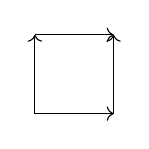
\begin{tikzpicture}[baseline=0.3cm]
\draw[->] (0,0)--(1,0);
\draw[->] (0,1)--(1,1);
\draw[->] (0,0)--(0,1);
\draw[->] (1,0)--(1,1);
\end{tikzpicture}
\end{description}

[In the right margin:]
\par\nopagebreak[4]
Here $\begin{matrix}\longrightarrow\\\longrightarrow\end{matrix}$ are horizontal morphisms,
$\uparrow\ \uparrow$ vertical morphisms.
(Their beginnings and ends are 1-morphisms.)

One can compose:
\begin{description}
\item[1)] $\longrightarrow\ \longrightarrow$ two horizontal morphisms
\item[2)] $\begin{matrix}\uparrow\\\uparrow\end{matrix}$ two vertical morphisms
\item[3)] squares are multiplied in two ways
\end{description}
\begin{center}
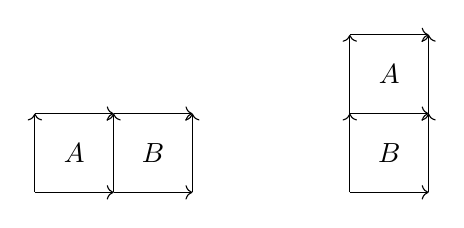
\begin{tikzpicture}
\draw[->] (0,0)--(1,0);
\draw[->] (1,0)--(2,0);
\draw[->] (0,1)--(1,1);
\draw[->] (1,1)--(2,1);
\draw[->] (0,0)--(0,1);
\draw[->] (1,0)--(1,1);
\draw[->] (2,0)--(2,1);
\node at (0.5,0.5) {$A$};
\node at (1.5,0.5) {$B$};
\draw[->] (4,0)--(5,0);
\draw[->] (4,1)--(5,1);
\draw[->] (4,2)--(5,2);
\draw[->] (4,0)--(4,1);
\draw[->] (4,1)--(4,2);
\draw[->] (5,0)--(5,1);
\draw[->] (5,1)--(5,2);
\node at (4.5,1.5) {$A$};
\node at (4.5,0.5) {$B$};
\end{tikzpicture}
\end{center}
(See Gabriel's book.)


\EnglishSourceFrame{GELFAND-P001406}{33}
\underline{The main nontrivial axiom}: two-dimensional associativity

(1)
\EnglishSourceFigure{GELFAND-P001406}{interchange-diagram}{On the left are two vertical rectangles: the first has $A$ above $B$, the second $C$ above a heavily retraced sign resembling $D$; the middle horizontal arrow in each points to the right. Between the rectangles is a composition circle, followed by an equals sign. On the right, the upper row contains $A$, $C$, the lower $B$ and a sign resembling $D$; between the rows is a narrow band with a circle. At the ends of the band are arrow-like and retraced strokes whose exact connections are unclear.}

\begin{center}
\begin{minipage}[t]{.46\linewidth}\vspace{0pt}\centering
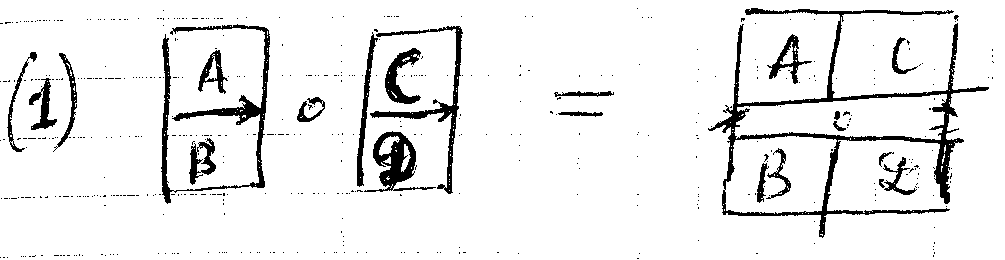
\includegraphics[width=\linewidth]{figures/gelfand-0153-p001406-interchange-original.png}\par\smallskip
{\footnotesize Original manuscript detail: \texttt{GELFAND-P001406}}
\end{minipage}\hfill
\begin{minipage}[t]{.50\linewidth}\vspace{0pt}\centering
{\footnotesize Partial visible-stroke recreation}\par\smallskip
\resizebox{\linewidth}{!}{% Visible-stroke transcription; D? and the retraced side connections remain unresolved.
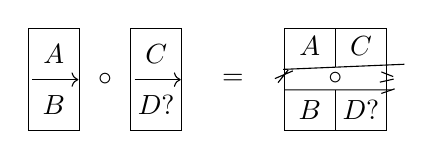
\begin{tikzpicture}[x=.65cm,y=.65cm]
\draw (0,0) rectangle (1,2); \draw[->] (.08,1)--(.98,1);
\node at (.5,1.5) {$A$};\node at (.5,.5) {$B$};
\node at (1.5,1) {$\circ$};
\draw (2,0) rectangle (3,2);\draw[->] (2.08,1)--(2.98,1);
\node at (2.5,1.5) {$C$};\node at (2.5,.5) {$D?$};
\node at (4,1) {$=$};
\draw (5,0)--(7,0)--(7,2)--(5,2)--cycle;
\draw (5,.8)--(7.1,.8) (4.98,1.2)--(7.35,1.3);
\draw (6,0)--(6,.8) (6,1.25)--(6,2);
\node at (5.5,1.65) {$A$};\node at (6.5,1.65) {$C$};
\node at (5.5,.4) {$B$};\node at (6.5,.4) {$D?$};
\node at (6,1.02) {$\circ$};
% Plain crossing strokes preserve uncertainty and do not declare arrows.
\draw (4.82,1.02)--(5.17,1.17) (4.88,.94)--(5.08,1.19);
\draw (6.9,1.15)--(7.13,1.06) (6.87,.95)--(7.14,1.01)
 (6.9,.73)--(7.16,.82);
\end{tikzpicture}
}
\end{minipage}
\end{center}
\noindent{\small\textit{The two D-like labels and retraced side strokes are unresolved. Plain side strokes do not declare arrow directions.}}


\underline{An example in which}
[crossed out: \EnglishUnclear{GELFAND-P001406}{example-cancel-left}{illegible}]
axiom
[crossed out: \EnglishUnclear{GELFAND-P001406}{example-cancel-right}{illegible}]
(1) \underline{does not hold}

\par\noindent\begin{minipage}{\linewidth}
\underline{Tensors:}
\begin{center}
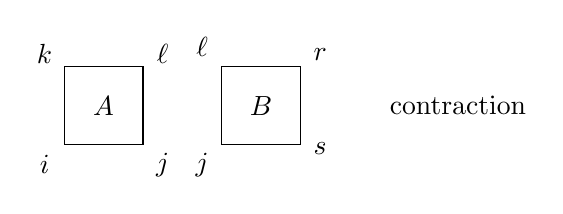
\begin{tikzpicture}
\draw (0,0)--(1,0)--(1,1)--(0,1)--cycle;
\node at (0.5,0.5) {$A$};
\node at (-0.25,1.15) {$k$};
\node at (1.25,1.15) {$\ell$};
\node at (-0.25,-0.25) {$i$};
\node at (1.25,-0.25) {$j$};
\draw (2,0)--(3,0)--(3,1)--(2,1)--cycle;
\node at (2.5,0.5) {$B$};
\node at (1.75,1.25) {$\ell$};
\node at (3.25,1.15) {$r$};
\node at (1.75,-0.25) {$j$};
\node at (3.25,-0.05) {$s$};
\node at (5,0.5) {contraction};
\end{tikzpicture}
\end{center}
\end{minipage}\par
\begin{equation*}
(AB)_{ik}^{rs}=\sum A_{ij}^{k\ell}B_{js}^{\ell r}
\end{equation*}
\EnglishUnclear{GELFAND-P001406}{tensor-indices}{The positions of the indices are retained from the manuscript.}

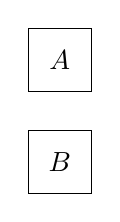
\begin{tikzpicture}
\draw (0,1.3)--(0.8,1.3)--(0.8,2.1)--(0,2.1)--cycle;
\node at (0.4,1.7) {$A$};
\draw (0,0)--(0.8,0)--(0.8,0.8)--(0,0.8)--cycle;
\node at (0.4,0.4) {$B$};
\end{tikzpicture}

Axiom (1) will not hold.

\underline{Another definition} (M. Kontsevich) (a competing one)

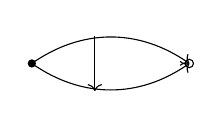
\begin{tikzpicture}[baseline=0cm]
\fill (0,0) circle (1.5pt);
\draw (2,0) circle (1.5pt);
\draw[->] (0,0) to[bend left=35] (2,0);
\draw[->] (0,0) to[bend right=35] (2,0);
\draw[->] (0.8,0.35)--(0.8,-0.35);
\end{tikzpicture}
Morphisms between morphisms with the same endpoints.

\underline{Example:} $Cat$ (the category of categories; there is a morphism
of functors)

This is a special case of the preceding definition (contract the vertical arrows).

\underline{I. M. G.}

\EnglishSourceFigure{GELFAND-P001406}{boundary-diagram}{Inside the square is written $\Delta u=0$. Along the upper and lower sides, horizontal arrows point to the right; beside the left side, two interior vertical arrows point upwards. On the left are the labels $u$ and $\frac{\partial u}{\partial n}$; above that label is another unclear notation.}

\begin{center}
\begin{minipage}[t]{.46\linewidth}\vspace{0pt}\centering
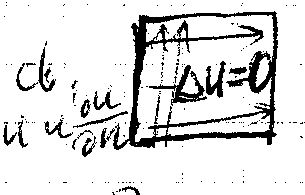
\includegraphics[width=\linewidth]{figures/gelfand-0153-p001406-boundary-original.png}\par\smallskip
{\footnotesize Original manuscript detail: \texttt{GELFAND-P001406}}
\end{minipage}\hfill
\begin{minipage}[t]{.50\linewidth}\vspace{0pt}\centering
{\footnotesize Partial visible-stroke recreation}\par\smallskip
\resizebox{\linewidth}{!}{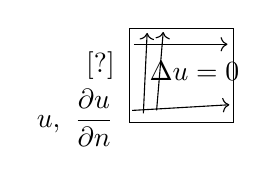
\begin{tikzpicture}[x=1.2cm,y=1.2cm]
\draw (0,0) rectangle (1.1,1);
\draw[->] (.05,.83)--(1.04,.83);\draw[->] (.03,.13)--(1.06,.19);
\draw[->] (.15,.1)--(.19,.95);\draw[->] (.29,.13)--(.36,.96);
\node at (.69,.55) {$\Delta u=0$};
\node[left] at (-.05,.6) {$[?]$};
\node[left] at (-.06,.05) {$u,\ \dfrac{\partial u}{\partial n}$};
\end{tikzpicture}
}
\end{minipage}
\end{center}
\noindent{\small\textit{The upper left notation remains [?] after 3×, 5× and 10× inspection. The visible u and normal derivative are typed; no boundary condition is supplied.}}

Boundary conditions

A request to Keldysh--Chentsov--Gelfand

\underline{K.} Higher fundamental groups.
$X_0\subset X_1\subset X$ is a topological space.

Objects are points $x\in X_0$.

Morphisms
$\bigl(\underset{\text{interval}}{I},\partial I\bigr)\longrightarrow(X_1,X_0)$;
homotopic ones $(\mathrm{mod}\ \partial I)$ are considered equivalent.

Bimorphisms
$(I^2,\partial I^2)\longrightarrow(X,X_1)$
\qquad $(\mathrm{mod}\ \text{\underline{homotopy}})$


\par\noindent\begin{minipage}{\linewidth}
\EnglishSourceFrame{GELFAND-P001407}{44}
\underline{\underline{23/XI-87.}} \qquad \underline{Gelfand seminar.}

\underline{Beilinson} (continued)

\underline{Derived categories.}

(1) \underline{Lemma:}
\begin{equation*}
\begin{tikzcd}[column sep=small,row sep=small]
X^\bullet && Y^\bullet\\
& Z^\bullet \arrow[ul,"{\text{quasi-isomorphism}}"] \arrow[ur] &
\end{tikzcd}
\quad\Rightarrow\quad\exists\quad
\begin{tikzcd}[column sep=small,row sep=small]
& Z'^\bullet &\\
X^\bullet \arrow[ur,"{\text{quasi-isomorphism}}"] && Y^\bullet \arrow[ul]
\end{tikzcd}
\end{equation*}
\end{minipage}\par

The lemma is proved using the mapping-cone construction.

\underline{Reminder:}

$\mathcal{A}$ is an abelian category.
\begin{equation*}
\begin{array}{ccccc}
C(\mathcal{A}) & \longrightarrow & K(\mathcal{A}) & \longrightarrow & D(\mathcal{A})\\
\text{complexes} && \substack{\text{homotopy}\\\text{category}\\\text{of complexes}} &&
\substack{\text{derived}\\\text{category}}
\end{array}
\end{equation*}
[On the right:] (the objects are complexes throughout).

$f:X^\bullet\to Y^\bullet$ is homotopic to $0$ if
$\exists g^i:X^i\to Y^{i-1}$,
\begin{equation*}
f^i=dg^i+g^{i+1}d
\end{equation*}

$D(\mathcal{A})$ is $K(\mathcal{A})$ with the
\underline{quasi-isomorphisms} inverted
(morphisms inducing isomorphisms of cohomology).

A morphism from $X^\bullet$ to $Y^\bullet$ is a diagram in $K(\mathcal{A})$:
\begin{equation*}
\begin{tikzcd}[column sep=small,row sep=small]
X^\bullet && Y^\bullet\\
& Z^\bullet \arrow[ul,"\sim"] \arrow[ur] &
\end{tikzcd}
\tag{2}
\end{equation*}
(The left arrow is a quasi-isomorphism.)

More precisely, an equivalence class of such diagrams: diagram (2) is equivalent to
the diagram obtained using any quasi-isomorphism
$\chi:Z'^\bullet\to Z^\bullet$:
\begin{equation*}
\begin{tikzcd}[column sep=small,row sep=small]
X^\bullet && Y^\bullet\\
& Z^\bullet \arrow[ul,"\varphi"',"\sim"] \arrow[ur,"\psi"] &\\
& Z'^\bullet \arrow[u,"\chi"',"\sim"] &
\end{tikzcd}
\qquad
\begin{tikzcd}[column sep=small,row sep=small]
X^\bullet && Y^\bullet\\
& Z' \arrow[ul,"{\varphi\circ\chi}"',"\sim"] \arrow[ur,"{\psi\circ\chi}"'] &
\end{tikzcd}
\tag{3}
\end{equation*}

(Extend this relation to the smallest equivalence relation containing it.)

The cone of a morphism and exact triangles were defined
[crossed out: \EnglishUnclear{GELFAND-P001407}{last-line-cancellation}{illegible}]
also [source final word: ``eshchyo''].


\EnglishSourceFrame{GELFAND-P001408}{unlabelled}
\underline{I. Zakharevich}
[crossed out: \EnglishUnclear{GELFAND-P001408}{cancelled-title}{illegible}]
\underline{Improvisation \EnglishUnclear{GELFAND-P001408}{title-preposition}{about / with} chaos.}

\underline{Examples}

$1^{\circ}$. Apparently there is a morphism from one example to the other.
\begin{equation*}
M=(\mathbb{Z}/2\mathbb{Z})^{\mathbb{Z}}
\qquad\text{(a sequence infinite in both directions)}
\end{equation*}
$T\colon M\to M$. On $M$ is the standard topology (a Cantor set).
\begin{equation*}
a_i\to a_{i-1}\qquad\text{(the shift transformation; the Bernoulli transformation)}
\end{equation*}
Consider the iterates: $T^N$.

There is a measure on $M$. The baker transformation coincides with this
[inserted above the line: (up to measure $0$)]
[crossed out after ``this'' and in the line below:
\EnglishUnclear{GELFAND-P001408}{baker-cancellations}{illegible}].

\begin{center}
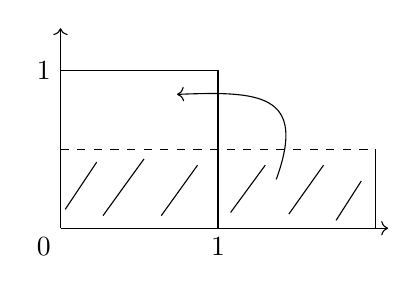
\begin{tikzpicture}[x=2cm,y=2cm]
\draw[->] (0,0) -- (2.08,0);
\draw[->] (0,0) -- (0,1.27);
\draw (0,1) -- (1,1) -- (1,0);
\draw (2,0) -- (2,0.5);
\draw[dashed] (0,0.5) -- (2,0.5);
\draw (0.03,0.12) -- (0.23,0.42);
\draw (0.27,0.08) -- (0.53,0.44);
\draw (0.64,0.08) -- (0.87,0.4);
\draw (1.08,0.1) -- (1.3,0.4);
\draw (1.45,0.09) -- (1.67,0.4);
\draw (1.75,0.05) -- (1.91,0.3);
\draw[->] (1.37,0.31) .. controls (1.57,0.86) and (1.26,0.87) .. (0.74,0.85);
\node[below left] at (0,0) {$0$};
\node[left] at (0,1) {$1$};
\node[below] at (1,0) {$1$};
\end{tikzpicture}
\end{center}

\EnglishSourceFigure{GELFAND-P001408}{baker-sequence}{Three drawings from left to right: a square with a closed rounded curve and a horizontal dashed line; a square with two elongated bends entering from opposite sides; a square with several nearly horizontal strips and short loop-shaped bends at the edges. The third drawing has a distinguishable left-pointing arrow on its lower long line; the directions of small strokes in the first and third drawings are not entirely clear.}

\begin{center}
\begin{minipage}[t]{.46\linewidth}\vspace{0pt}\centering
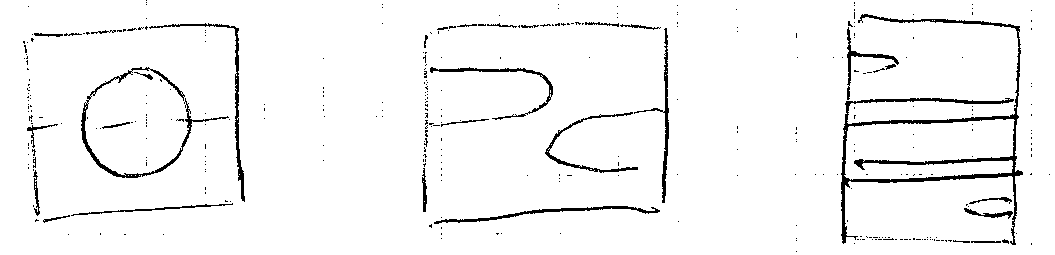
\includegraphics[width=\linewidth]{figures/gelfand-0153-p001408-baker-sequence-original.png}\par\smallskip
{\footnotesize Original manuscript detail: \texttt{GELFAND-P001408}}
\end{minipage}\hfill
\begin{minipage}[t]{.50\linewidth}\vspace{0pt}\centering
{\footnotesize Partial visible-stroke recreation}\par\smallskip
\resizebox{\linewidth}{!}{% Only the clear leftward long arrow is interpreted as a direction.
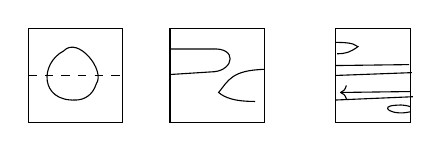
\begin{tikzpicture}[x=.6cm,y=.6cm]
\draw (0,0) rectangle (2,2);\draw[dashed] (0,1)--(2,1);
\draw (1,.48) .. controls (.25,.45) and (.24,1.25) .. (.75,1.52)
 .. controls (1.05,1.84) and (1.64,1.11) .. (1.44,.82)
 .. controls (1.36,.57) and (1.17,.48) .. (1,.48);
\draw (3,0) rectangle (5,2);
\draw (3,1.56)--(3.88,1.56) .. controls (4.44,1.6) and (4.35,1.12) .. (3.94,1.08)--(3,1.02);
\draw (5,1.13) .. controls (4.31,1.11) and (4.24,.9) .. (4.03,.64)
 .. controls (4.16,.53) and (4.36,.45) .. (4.8,.45);
\draw (6.5,0) rectangle (8.1,2);
\draw (6.5,1.7) .. controls (6.93,1.7) and (6.9,1.64) .. (6.98,1.61)
 .. controls (6.81,1.49) and (6.72,1.46) .. (6.54,1.46);
\draw (6.5,1.21)--(8.06,1.23) (6.5,1.0)--(8.12,1.06);
\draw[->] (8.1,.66)--(6.6,.64);\draw (6.5,.48)--(8.14,.55);
\draw (8.08,.23) .. controls (7.7,.14) and (7.4,.35) .. (7.78,.37)
 .. controls (7.93,.39) and (8.07,.35) .. (8.08,.34);
\end{tikzpicture}
}
\end{minipage}
\end{center}
\noindent{\small\textit{Visible bends are preserved. Only the clear long left-pointing arrow is assigned a direction; small endpoint strokes remain uninterpreted.}}

And so on.

\underline{Correspondence}: write the coordinates of a point of the square in binary
and take $1$ digit to the left, another to the right.

In what sense is this chaos?

Consider $T^k x$, $k\leq 0$; suppose this is known (to within $1$ mm).
\begin{equation*}
T^k x,\qquad k>0
\end{equation*}
In finite time, all this information will be lost.

$2^{\circ}$. \underline{Hyperbolic transformation}:
geodesic flows on \EnglishUnclear{GELFAND-P001408}{manifold-abbreviation}{mn-ziyakh / mn-iyakh [unexpanded source abbreviations]} of negative curvature.

\EnglishSourceFigure{GELFAND-P001408}{hyperbolic-surface}{A closed contour with two expanded parts and a constriction between them. Inside, on the left and right, arcs resemble indications of two handles of a surface; the middle contains a short slanting segment with marked endpoints and a branching arrow upwards to the right. Small directions and the exact connections of the interior arcs require comparison with the original.}

\begin{center}
\begin{minipage}[t]{.46\linewidth}\vspace{0pt}\centering
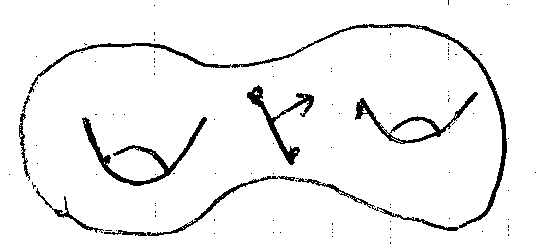
\includegraphics[width=\linewidth]{figures/gelfand-0153-p001408-hyperbolic-surface-original.png}\par\smallskip
{\footnotesize Original manuscript detail: \texttt{GELFAND-P001408}}
\end{minipage}\hfill
\begin{minipage}[t]{.50\linewidth}\vspace{0pt}\centering
{\footnotesize Partial visible-stroke recreation}\par\smallskip
\resizebox{\linewidth}{!}{% The drawn contour and interior arcs are reproduced without a genus assertion.
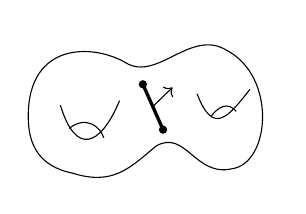
\begin{tikzpicture}[x=.8cm,y=.8cm]
\draw (0,1) .. controls (0,2.2) and (1.05,2.15) .. (1.55,1.85)
 .. controls (2.05,1.55) and (2.58,2.4) .. (3.15,2.05)
 .. controls (3.95,1.63) and (3.84,.26) .. (3.24,.17)
 .. controls (2.65,.03) and (2.5,.8) .. (2.03,.53)
 .. controls (1.6,.17) and (1.34,-.1) .. (.7,.1)
 .. controls (.17,.21) and (0,.55) .. (0,1);
\draw (.51,1.18) .. controls (.75,.38) and (1.14,.51) .. (1.45,1.25);
\draw (.65,.81) .. controls (.92,1.02) and (1.14,.84) .. (1.2,.66);
\draw (2.68,1.36) .. controls (2.94,.68) and (3.18,1.0) .. (3.52,1.43);
\draw (2.91,1.01) .. controls (3.09,1.24) and (3.23,1.17) .. (3.3,1.08);
\draw[very thick] (1.82,1.51)--(2.14,.79);
\fill (1.82,1.51) circle (1.5pt);\fill (2.14,.79) circle (1.5pt);
\draw[->] (1.97,1.15)--(2.29,1.46);
\end{tikzpicture}
}
\end{minipage}
\end{center}
\noindent{\small\textit{The outer contour, interior arcs, marked segment and branch arrow are recreated. No topology or metric is inferred from the sketch.}}



\EnglishSourceFrame{GELFAND-P001409}{45}
\underline{G. Margulis.}
\underline{Iterates of maps of the complex plane.}

Consider the transformation $z\to P(z)$, where $P$ is a polynomial

(more generally, a rational function).

$\operatorname{deg}P=1$
[crossed out: \EnglishUnclear{GELFAND-P001409}{degree-one-cancellation}{illegible}]
is an uninteresting case.

$(1)\quad z\mapsto az+b$

\underline{Iterates}:
\begin{equation*}
z_{i+1}=P(z_i)
\end{equation*}
$|a|>1\Rightarrow$ one fixed point;

\EnglishUnclear{GELFAND-P001409}{unit-modulus-claim}{$|a|=1\Rightarrow$ everything splits into invariant circles, on which there is a rotation.}

\begin{center}
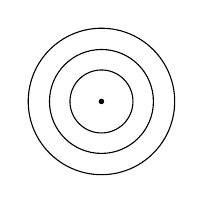
\begin{tikzpicture}
\draw (0,0) circle (0.4);
\draw (0,0) circle (0.66);
\draw (0,0) circle (0.93);
\fill (0,0) circle (0.035);
\end{tikzpicture}
\end{center}

\underline{I. M. G.}: 1) The question of when a transformation of the circle is diffeomorphic to a rotation
is nontrivial: Denjoy, Arnold, Herman.

2) What is a representation of a discrete infinite group?

There is no satisfactory answer.

Von Neumann theory is not aesthetically pleasing.

Chaos arises on the circle.

\underline{Conjecture}: if one works with sets of intermediate Hausdorff
dimension, some classical theory will be restored!!

\underline{Question for schoolchildren}: cover the $n$th rational number by an interval
of length $\varepsilon/2^n$. Give an example of a number which will not be covered.

\underline{Problem}: find the Hausdorff dimension of the Cantor perfect set.

\tikz\node[draw,circle,inner sep=2pt] {!};
\underline{Problem}. \underline{Construct a representation theory of discrete groups on functions on}
\underline{sets of intermediate Hausdorff dimension.}

To begin with, look at physics---string theory and so on.

\underline{G. M.}:
$z\to z^2$
\qquad $|z|=1$ maps to itself.

\begin{center}
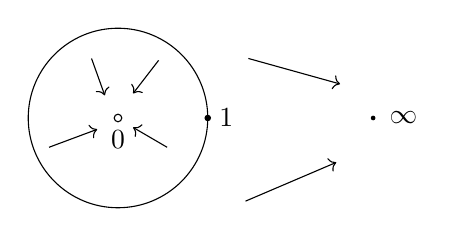
\begin{tikzpicture}[x=1.2cm,y=1.2cm]
\draw (0,0) circle (0.95);
\draw (0,0) circle (0.04);
\node[below] at (0,-0.03) {$0$};
\fill (0.95,0) circle (0.035);
\node[right] at (0.97,0) {$1$};
\draw[->] (-0.28,0.63) -- (-0.14,0.24);
\draw[->] (0.43,0.61) -- (0.16,0.26);
\draw[->] (0.52,-0.31) -- (0.16,-0.1);
\draw[->] (-0.73,-0.31) -- (-0.22,-0.12);
\draw[->] (1.38,0.63) -- (2.35,0.36);
\draw[->] (1.35,-0.88) -- (2.31,-0.47);
\fill (2.7,0) circle (0.025);
\node[right] at (2.77,0) {$\infty$};
\end{tikzpicture}
\end{center}
On the circle, this is an analogue of the (one-sided)
baker transformation.


\EnglishSourceFrame{GELFAND-P001410}{unlabelled}
\begin{equation*}
f_n=\underbrace{f\circ f\circ\cdots\circ f}_{n\ \text{times}}
\end{equation*}
\underline{Definition}

$U$ is a [crossed out: set; inserted above the line: neighbourhood]
of normality if $\left.f_n\right|_U$ is a compact set

(a normal family of analytic functions).

[On a separate short line, crossed out:
\EnglishUnclear{GELFAND-P001410}{isolated-cancellation}{illegible}.]

The set of normality [inserted above the line: $X$] consists of points $x$ for which
$\exists$ a neighbourhood $U$---[crossed out:
\EnglishUnclear{GELFAND-P001410}{normality-cancellation}{illegible}]
a neighbourhood of normality.

[Beneath ``set of normality'': (it is open).]

The complement of the set of normality is the \underline{Julia set}.

(It is closed.)

The set of normality may be empty.

\begin{equation*}
X=X_1\cup\cdots\cup X_n\cup\cdots
\end{equation*}
(connected components)

of the set of normality

[crossed out beneath this caption:
\EnglishUnclear{GELFAND-P001410}{components-cancellation}{illegible}]

\begin{equation*}
\begin{aligned}
f\colon (\text{connected components})&\to(\text{connected components})\\
X_i&\mapsto X_{j(i)}
\end{aligned}
\end{equation*}
\underline{Sullivan} proved that in the resulting

[crossed out: \EnglishUnclear{GELFAND-P001410}{sullivan-cancellation}{illegible}]
transformation of a discrete set (countable or finite),

a) every orbit stabilises,

b) the set of fixed points is finite.

\underline{Idea of the proof}. Suppose that there is an infinite orbit.

\begin{center}
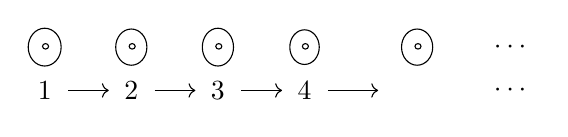
\begin{tikzpicture}[x=1.1cm,y=1cm]
\draw (0,0) ellipse (0.19 and 0.24);
\draw (0.01,0.01) circle (0.035);
\draw (1,0) ellipse (0.18 and 0.23);
\draw (1.01,0.01) circle (0.035);
\draw (2,0) ellipse (0.18 and 0.24);
\draw (2.01,0.01) circle (0.035);
\draw (3,0) ellipse (0.17 and 0.22);
\draw (3.01,0.01) circle (0.035);
\draw (4.3,0) ellipse (0.18 and 0.23);
\draw (4.31,0.01) circle (0.035);
\node at (5.4,0) {$\cdots$};
\node at (0,-0.55) {$1$};
\node at (1,-0.55) {$2$};
\node at (2,-0.55) {$3$};
\node at (3,-0.55) {$4$};
\draw[->] (0.27,-0.55) -- (0.74,-0.55);
\draw[->] (1.27,-0.55) -- (1.74,-0.55);
\draw[->] (2.27,-0.55) -- (2.74,-0.55);
\draw[->] (3.27,-0.55) -- (3.85,-0.55);
\node at (5.4,-0.55) {$\cdots$};
\end{tikzpicture}
\end{center}

Make a change of conformal
[crossed out: \EnglishUnclear{GELFAND-P001410}{structure-cancellation}{transf. [source abbreviation] / illegible}]
structure, so that the transformation remains
conformal.

\underline{Problem}:

\EnglishSourceFigure{GELFAND-P001410}{circle-packing}{Inside a square are four large rounded contours, two in the upper and two in the lower row; smaller closed curves occupy the gaps and border. On the right, a horizontal arrow points towards the square, with the caption ``inscribe''. Exact tangencies and which contours contain small boundary arcs are not entirely distinguishable.}

\def\GelfandPackingCaption{inscribe}
\begin{center}
\begin{minipage}[t]{.46\linewidth}\vspace{0pt}\centering
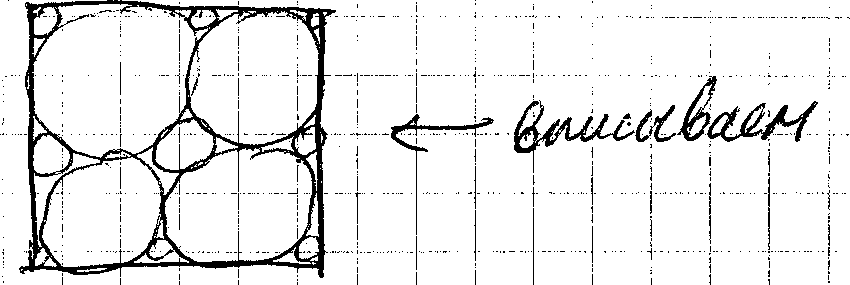
\includegraphics[width=\linewidth]{figures/gelfand-0153-p001410-circle-packing-original-r2.png}\par\smallskip
{\footnotesize Original manuscript detail: \texttt{GELFAND-P001410}}
\end{minipage}\hfill
\begin{minipage}[t]{.50\linewidth}\vspace{0pt}\centering
{\footnotesize Partial visible-stroke recreation}\par\smallskip
\resizebox{\linewidth}{!}{% Hand-drawn contours; these coordinates do not specify exact tangencies or radii.
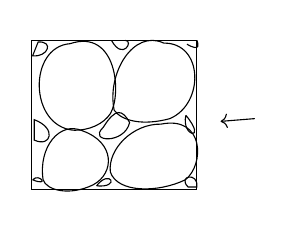
\begin{tikzpicture}[x=.7cm,y=.7cm]
\draw (0,0) rectangle (3,2.7);
\draw (.75,1.07) .. controls (-.05,1.16) and (-.06,2.58) .. (.7,2.64)
 .. controls (1.55,2.92) and (1.64,1.72) .. (1.43,1.37)
 .. controls (1.31,1.19) and (1.06,1.06) .. (.75,1.07);
\draw (1.5,1.43) .. controls (1.36,2.1) and (1.85,2.91) .. (2.4,2.65)
 .. controls (3.12,2.66) and (3.14,1.55) .. (2.51,1.28)
 .. controls (2.03,1.15) and (1.65,1.23) .. (1.5,1.43);
\draw (.21,.17) .. controls (.12,.76) and (.51,1.24) .. (.92,1.06)
 .. controls (1.52,.85) and (1.51,.29) .. (1.12,.08)
 .. controls (.69,-.13) and (.27,-.02) .. (.21,.17);
\draw (1.43,.31) .. controls (1.38,.73) and (1.84,1.19) .. (2.35,1.18)
 .. controls (3.14,1.34) and (3.14,.44) .. (2.79,.17)
 .. controls (2.29,-.07) and (1.56,-.07) .. (1.43,.31);
\draw (.02,2.42) .. controls (.3,2.39) and (.41,2.69) .. (.12,2.67)--cycle;
\draw (1.45,2.7) .. controls (1.66,2.32) and (1.86,2.7) .. (1.7,2.7);
\draw (2.82,2.63) .. controls (3.08,2.48) and (3.02,2.65) .. (3,2.7);
\draw (.05,.89) .. controls (.36,.75) and (.46,1.11) .. (.05,1.26)--cycle;
\draw (1.3,1.12) .. controls (1.01,.85) and (1.69,.81) .. (1.78,1.21)
 .. controls (1.65,1.44) and (1.53,1.49) .. (1.3,1.12);
\draw (2.8,1.34) .. controls (3.2,.86) and (2.71,.94) .. (2.8,1.34);
\draw (.02,.17) .. controls (.34,.04) and (.14,.3) .. (.02,.17);
\draw (1.18,.06) .. controls (1.42,.38) and (1.63,.02) .. (1.18,.06);
\draw (2.84,.04) .. controls (2.64,.24) and (3.03,.32) .. (3,.04)--cycle;
\draw[->] (4.05,1.28)--(3.43,1.23);
\node[right] at (4.05,1.28) {\GelfandPackingCaption};
\end{tikzpicture}
}
\end{minipage}
\end{center}
\noindent{\small\textit{The visible contours are recreated approximately. Exact tangencies, circle sizes and the inclusion of small boundary arcs remain unresolved; the reconstruction specifies no quantitative packing.}}


1) Prove that the remainder has measure $0$.

2) Prove that the remainder has Hausdorff dimension $<2$.


\EnglishSourceFrame{GELFAND-P001411}{46}
\underline{\underline{I. M. Gelfand}}. \underline{Matroids.}

In a $K$-dimensional space, consider $n$ vectors;
enumerate them and compile a list of which are linearly dependent and which are not.
Specifying this list gives a \underline{matroid}.

What conditions must this list satisfy?

\underline{Example}:
[Crossed out: \EnglishUnclear{GELFAND-P001411}{example-cancelled}{illegible}.]

\begin{center}
\begin{minipage}[t]{.46\linewidth}\vspace{0pt}\centering
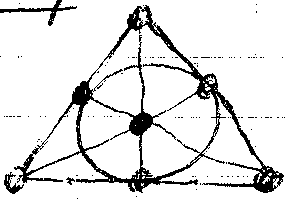
\includegraphics[width=\linewidth]{figures/gelfand-0153-p001411-fano-points-original.png}\par\smallskip
{\footnotesize Original manuscript detail: \texttt{GELFAND-P001411}}
\end{minipage}\hfill
\begin{minipage}[t]{.50\linewidth}\vspace{0pt}\centering
{\footnotesize Partial visible-stroke recreation}\par\smallskip
\resizebox{\linewidth}{!}{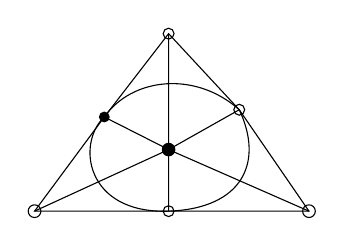
\begin{tikzpicture}[scale=1.15]
\coordinate (a) at (0,1.96);
\coordinate (b) at (-1.48,0);
\coordinate (c) at (1.55,0);
\coordinate (d) at (-0.71,1.04);
\coordinate (e) at (0.78,1.12);
\coordinate (f) at (0,0);
\coordinate (g) at (0,0.68);
\draw (a)--(d)--(b)--(f)--(c)--(e)--cycle;
\draw (a)--(g)--(f) (b)--(g)--(e) (d)--(g)--(c);
\draw (d) .. controls (-0.40,1.48) and (0.30,1.55) .. (e)
 .. controls (1.05,0.55) and (0.83,0.03) .. (f)
 .. controls (-0.92,-0.03) and (-1.02,0.75) .. (d);
\draw (a) circle (0.06) (b) circle (0.07) (c) circle (0.07)
 (e) circle (0.06) (f) circle (0.06);
\fill (d) circle (0.06) (g) circle (0.075);
\end{tikzpicture}
}
\end{minipage}
\end{center}
\noindent{\small\textit{The seven points retain the two filled and five outlined markings of the diplomatic drawing. No vector labels are added.}}


If three points lie on one line, the vectors
are linearly dependent.

The whole space is three-dimensional (there are no four linearly independent vectors).

(1) \underline{Problem}: 1) Prove that such vectors do not exist over $\mathbb{R}$ and $\mathbb{C}$!

2) Such vectors do exist over $\mathbb{Z}/2\mathbb{Z}$.

(All nonzero vectors in $(\mathbb{Z}/2\mathbb{Z})^3$!)

\underline{General} (\underline{unsolved problem}): which matroids are realised
a) over $\mathbb{R}$,
b) over $\mathbb{C}$.?

\underline{Solved problem}: which matroids are realised over $\forall$ fields?

\underline{In Rota's book} \EnglishUnclear{GELFAND-P001411}{book-after-rota}{e.. [source Cyrillic sign]}
[On the right: see \EnglishUnclear{GELFAND-P001411}{book-overwritten-noun}{book? [uncertain source ending]} \underline{Aigner} (?)]
there are fifteen different equivalent definitions of a matroid.

(2) \underline{Axioms}.

Certain subsets are distinguished and \underline{called bases}.

$B_1,B_2$ are two bases.

$y\in B_2,\ y\notin B_1\ \Rightarrow\ \exists x\in B_1;$
$(B_1\setminus x)\cup y$
[Crossed out: \EnglishUnclear{GELFAND-P001411}{basis-exchange-cancelled}{illegible}],
$(B_2\setminus y)\cup x$ are
\newline
bases.

\underline{Exercise in linear algebra}: verify this for a set of vectors in a vector space.

(3) \underline{Bimatroid}: consider a matrix; it defines two matroids, from its columns
and rows:

$S$ and $T$.

Another notion: list all minors $\ne0$.

Bimatroid: a family of subsets with the same number of elements.

(4) [Crossed out: \EnglishUnclear{GELFAND-P001411}{problem-four-cancelled}{illegible}.]
\underline{Problem}: state axioms for a bimatroid.


\EnglishSourceFrame{GELFAND-P001412}{unlabelled}
(5) \underline{Problem}: how is the bimatroid notion from
[Crossed out: \EnglishUnclear{GELFAND-P001412}{top-cancelled}{illegible}]
Gelfand--Serganova (UMN)
related to \EnglishUnclear{GELFAND-P001412}{knuth-name}{Kunt [source candidate: «Кунтом»]}?

\underline{Problem}: prove that

\begin{equation*}
\text{(6)}\quad
[x_1,\ldots,x_d][y_1,\ldots,y_d]
=\sum(-1)^{d-i}[y_1,x_2,\ldots,x_d]
[y_1,\ldots,y_{i-1},x_i,y_{i+1},\ldots,y_d]
\end{equation*}
\EnglishUnclear{GELFAND-P001412}{determinant-formula-source}{The indices $y_1$, $x_i$ and sign $(-1)^{d-i}$ are as in the manuscript.}

$[x_1,\ldots,x_d]$ is the determinant formed from the vectors.

(7) \underline{Remark}: if $[x_1,\ldots,x_d]$, $[y_1,\ldots,y_d]$ are bases, the right side has
a nonzero summand; this gives the exchange axiom
\EnglishUnclear{GELFAND-P001412}{basis-axiom-reference}{(3)}.

(\EnglishUnclear{GELFAND-P001412}{overwritten-eight}{8})
\underline{Problem} (tedious). Hilbert's chain of syzygies:
\begin{equation*}
(\text{ring})\longmapsto
\underset{\text{--- determinants}}{(\text{generators})}
\longmapsto (\text{relations between generators})
\end{equation*}

(9) (\underline{Assertion}: (6) gives all relations between the generators.)

(10) a) Write the whole chain!

b) Discretise the whole chain (write combinatorial relations).

(11) \underline{Problem}. A bimatroid---a list of minors $\longrightarrow$
[Crossed out: \EnglishUnclear{GELFAND-P001412}{problem-eleven-cancelled}{illegible}]
two matroids
(rows and columns).

A bimatroid is constructed from two matroids.

\EnglishSourceFigure{GELFAND-P001412}{basis-grid}{A grid of four vertical and four horizontal lines; braces on the left and below carry labels ``baz...'' [source beginnings]; an arrow on the right points leftwards towards the grid.}

\def\GelfandBasisLabel{baz... [?]}
\begin{center}
\begin{minipage}[t]{.46\linewidth}\vspace{0pt}\centering
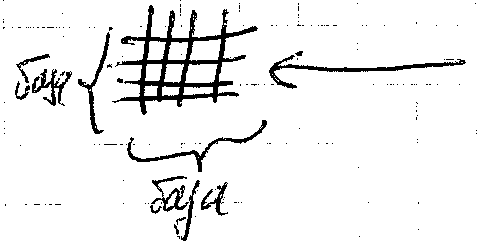
\includegraphics[width=\linewidth]{figures/gelfand-0153-p001412-basis-grid-original.png}\par\smallskip
{\footnotesize Original manuscript detail: \texttt{GELFAND-P001412}}
\end{minipage}\hfill
\begin{minipage}[t]{.50\linewidth}\vspace{0pt}\centering
{\footnotesize Partial visible-stroke recreation}\par\smallskip
\resizebox{\linewidth}{!}{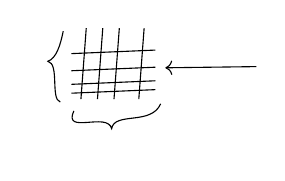
\begin{tikzpicture}[x=.75cm,y=.75cm]
\foreach \x in {0,.28,.56,.98}{\draw (\x,-.1)--(\x+.09,1.1);}
\foreach \y in {0,.15,.38,.67}{\draw (-.16,\y)--(1.26,\y+.06);}
\draw (-.3,1.05) .. controls (-.35,.8) and (-.42,.59) .. (-.56,.54)
 .. controls (-.36,.5) and (-.52,-.1) .. (-.35,-.15);
\draw (-.12,-.3) .. controls (-.31,-.71) and (.45,-.31) .. (.52,-.6)
 .. controls (.57,-.31) and (1.19,-.55) .. (1.35,-.18);
\node[left] at (-.58,.5) {\GelfandBasisLabel};
\node[below] at (.6,-.68) {\GelfandBasisLabel};
\draw[->] (2.97,.45)--(1.43,.43);
\end{tikzpicture}
}
\end{minipage}
\end{center}
\noindent{\small\textit{Both brace labels retain only the source beginning baz...; their endings remain unresolved after 3×, 5× and 10× inspection. Row and column basis terminology does not settle their glyphs.}}


by the definition of \EnglishUnclear{GELFAND-P001412}{basis-construction-word}{baza? [unresolved source form]}.

But this is not necessarily so.

A bimatroid contains more information.

What is the additional information in a bimatroid?

This is an important cohomological notion.

\underline{Remark}. Algebraic topology is a small island in familiar
combinatorial techniques.


\EnglishSourceFrame{GELFAND-P001413}{unlabelled}
\underline{\underline{30/XI-87.}}\qquad \underline{Gelfand seminar.}

\underline{I. M. Gelfand.} Problem: find the characters of the symmetric group.

(Following Frobenius.)

\underline{On the paper by} \underline{Kerov}: ``\underline{Realisation of representations of the Hecke algebra}, etc.''

Hint: these are characters of the symmetric group.

The Hecke algebra is the algebra with generators $\{e_k\}$
[above the line: $k=1,\ldots,N-1$] and relations
\begin{equation*}
\text{(1)}\quad
\left\{\begin{aligned}
e_k e_{k+1}e_k-\tau e_k&=e_{k+1}e_k e_{k+1}-\tau e_{k+1}\\
e_{k+j}e_k&=e_k e_{k+j},\quad j\geq 2;\\
e_k^2&=e_k
\end{aligned}\right.
\end{equation*}
Other generators
\begin{equation*}
\text{(2)}\quad \sigma_k=(q+1)e_k-1,\qquad \tau=\frac{q}{(q+1)^2}
\end{equation*}
This algebra is denoted by $H_N(q)$.

\underline{Exercise}: write the relations for $\sigma_k$.

(3) For $q=1$ (or $\tau=\frac14$), one obtains the group algebra of the symmetric group.

(4) \underline{Problem}: $\dim H_N(q)=N!$

[In the left margin: a circled ``!''.]
In the paper by \EnglishUnclear{GELFAND-P001413}{citation-name}{Tipper / Dipper} and James,

Proc. London Math. Soc.\qquad 1986, v. 52, p. 20--52

Recommended!!

it is proved that the representation theory of $H_N(q)$ is analogous to the theory of modular
representations of the symmetric group.

This works even in the complex case (see the paper by Bernsh.--Gelf.--Gelf.
on Verma modules).

Here it is assumed that $q\ne\sqrt[m]{1}$.

\underline{Construction of representations.}

A Young diagram\quad $\lambda=(\lambda_1,\lambda_2,\ldots,\lambda_k)$

\begin{center}
(5)\qquad
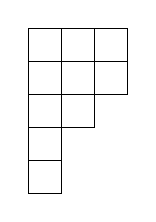
\begin{tikzpicture}[x=0.42cm,y=0.42cm]
\draw (0,0)--(3,0)--(3,-2)--(2,-2)--(2,-3)--(1,-3)--(1,-5)--(0,-5)--cycle;
\draw (1,0)--(1,-5);
\draw (2,0)--(2,-3);
\draw (0,-1)--(3,-1);
\draw (0,-2)--(3,-2);
\draw (0,-3)--(2,-3);
\draw (0,-4)--(1,-4);
\end{tikzpicture}
\qquad
$\begin{gathered}\sum\lambda_j=|\lambda|\\[8pt]\lambda_{i+1}\leq\lambda_i\end{gathered}$
\end{center}

($\lambda_i$ is the number of cells in the $i$th column.)

This corresponds to a conjugacy class of elements.


\EnglishSourceFrame{GELFAND-P001414}{52}
A Young tableau:
\begin{equation*}
\text{(6)}\quad t=\{\lambda^{(k)}\}_{k=1}^{N}
\quad\text{--- a family of diagrams in which}
\end{equation*}
\begin{equation*}
|\lambda^{(k)}|=k.
\end{equation*}

The usual definition (a different one): the tableau is filled with the numbers $1,2,\ldots,|\lambda|$, with
\begin{equation*}
\begin{matrix}\rightarrow\\\downarrow\end{matrix}
\quad\text{increase in these directions}
\end{equation*}

\begin{center}
\begin{minipage}[t]{.46\linewidth}\vspace{0pt}\centering
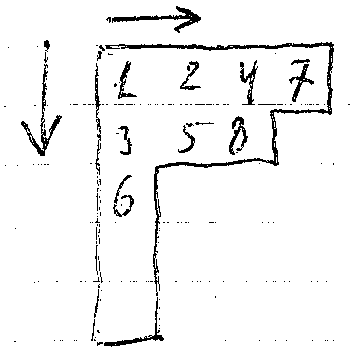
\includegraphics[width=\linewidth]{figures/gelfand-0153-p001414-young-tableau-original.png}\par\smallskip
{\footnotesize Original manuscript detail: \texttt{GELFAND-P001414}}
\end{minipage}\hfill
\begin{minipage}[t]{.50\linewidth}\vspace{0pt}\centering
{\footnotesize Partial visible-stroke recreation}\par\smallskip
\resizebox{\linewidth}{!}{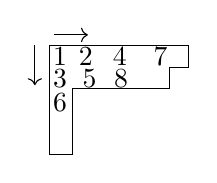
\begin{tikzpicture}[x=0.44cm,y=0.44cm]
\draw (0,0)--(4,0)--(4,-0.65)--(3.45,-0.65)--(3.45,-1.25)--(0.65,-1.25)--(0.65,-3.15)--(0,-3.15)--cycle;
\node at (0.30,-0.33) {$1$};
\node at (1.04,-0.33) {$2$};
\node at (2.02,-0.33) {$4$};
\node at (3.20,-0.33) {$7$};
\node at (0.30,-0.97) {$3$};
\node at (1.15,-0.97) {$5$};
\node at (2.06,-0.97) {$8$};
\node at (0.30,-1.66) {$6$};
\draw[->] (0.12,0.30)--(1.10,0.30);
\draw[->] (-0.43,0.0)--(-0.43,-1.15);
\end{tikzpicture}
}
\end{minipage}
\end{center}
\noindent{\small\textit{The irregular outline and the eight visible numbers are retained. The blank long leg is not filled and no internal cell grid is supplied.}}


In (6), they must increase.

\begin{center}
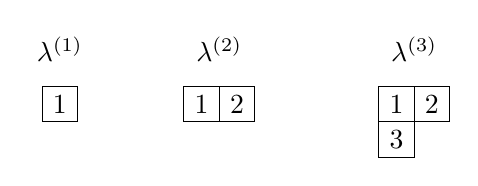
\begin{tikzpicture}[x=0.45cm,y=0.45cm]
\node at (0.5,1.05) {$\lambda^{(1)}$};
\draw (0,0) rectangle (1,-1);
\node at (0.5,-0.5) {$1$};
\node at (5,1.05) {$\lambda^{(2)}$};
\draw (4,0) rectangle (6,-1);
\draw (5,0)--(5,-1);
\node at (4.5,-0.5) {$1$};
\node at (5.5,-0.5) {$2$};
\node at (10.5,1.05) {$\lambda^{(3)}$};
\draw (9.5,0)--(11.5,0)--(11.5,-1)--(10.5,-1)--(10.5,-2)--(9.5,-2)--cycle;
\draw (10.5,0)--(10.5,-1);
\draw (9.5,-1)--(10.5,-1);
\node at (10,-0.5) {$1$};
\node at (11,-0.5) {$2$};
\node at (10,-1.5) {$3$};
\end{tikzpicture}
\end{center}

\begin{equation*}
\text{(7)}\quad r_k(t)=(i_{k+1}-j_{k+1})-(i_k-j_k)
\end{equation*}
The point $k$ has coordinates $(i_k,j_k)$.

For a diagram:
\begin{equation*}
\text{(8)}\quad h(\lambda)=r_\lambda+1
\end{equation*}
\begin{equation*}
\text{(9)}\quad r_\lambda=\max_{t\in T(\lambda)}\max_{1\leq k<N}|r_k(t)|,
\end{equation*}
where $T(\lambda)$ is the set of tableaux constructed from the diagram $\lambda$, i.e.
having shape $\lambda$.

Let $s=(\mu^{(k)})_{k=1}^{N}$,\quad $t=(\lambda^{(k)})_{k=1}^{N}$.

(10) \underline{Definition.}\quad $s\underset{n}{\approx}t$ if $\lambda^{(k)}=\mu^{(k)}$, $k\ne n$.

\underline{Assertion.}

(11) [Crossed out: \EnglishUnclear{GELFAND-P001414}{eq11-cancelled-word}{if?};
inserted above the line: Let]
$r_n(t)=\pm1$; then $s\underset{n}{\approx}t\Rightarrow s=t$;

(12) Let $|r_n(t)|>1$; then $\exists!\ s:\quad s\underset{n}{\approx}t$, $s\ne t$.

\begin{equation*}
\text{(13)}\quad S_\lambda^{(k)}=\Vert S_{s,t}^{(k)}(\tau)\Vert_{s,t\in T(\lambda)}
\quad\text{--- a matrix};
\end{equation*}
[After the matrix index, below the line:
\EnglishUnclear{GELFAND-P001414}{eq13-terminal-mark}{an illegible sign; $q$ / a corrected comma}.]

\begin{equation*}
\text{(14)}\quad
S_{s,t}^{(k)}(\tau)=\bigl(W_{r_k(s)}(\tau)\ W_{r_k(t)}(\tau)\bigr)^{1/2}
\quad\text{for }s\underset{k}{\approx}t
\end{equation*}
[After the first factor, below the line:
\EnglishUnclear{GELFAND-P001414}{eq14-blotted-mark}{a blotted or crossed-out sign}.]

[Crossed out: \EnglishUnclear{GELFAND-P001414}{eq14-cancelled-condition}{for $s\underset{k}{\approx}t$?}]
and $S_{s,t}^{(k)}(\tau)=0$ otherwise.

\EnglishSourceFrame{GELFAND-P001415}{unlabelled}
(15) \underline{Theorem}. Let $\lambda$ be a diagram with $N$ elements and
$q\ne\sqrt[m]{1}$. Then $S_{\lambda}^{(k)}$ define a representation of the Hecke algebra
(in the generators $e_k$).

We shall construct the functions $W$.
$W_{-r}(\tau)$ for $r=1,2,\ldots$ are defined by the relations
\begin{equation}
 W_{-(r+1)}(\tau)=1-\frac{\tau}{W_{-r}(\tau)},\qquad r\geq0,
 \tag{16}
\end{equation}
[Crossed out: \EnglishUnclear{GELFAND-P001415}{eq16-cancelled}{and for $r\ne0$; possibly $r\geq0$.}]
\begin{equation}
 W_r(\tau)=1-W_{-r}(\tau),\qquad r\geq0;
 \tag{17}
\end{equation}

Or:

$W_{-r}(\tau)$ is defined
[Crossed out: \EnglishUnclear{GELFAND-P001415}{continued-fraction-cancelled-word}{illegible}]
by the continued-fraction expansion:
\begin{equation}
 \text{[Crossed out: }W_{-r}(\tau)=\text{]}\quad
 1-\frac{\tau}{1-\dfrac{\tau}{1-\ldots}}
 \tag{18}
\end{equation}
There is the equation:
\begin{equation}
 W_r(\tau)W_{1-r}(\tau)=1.
 \tag{19}
\end{equation}
\EnglishUnclear{GELFAND-P001415}{eq19-right-hand-side}{The right side is written as $1$.}

General formula:
\begin{equation}
 W_r(\tau)=\frac{q(q^{r-1}-1)}{(q+1)(q^r-1)},\qquad r=1,2,\ldots
 \tag{20}
\end{equation}
\begin{equation}
 W_{-r}(\tau)=\frac{q^{r+1}-1}{(q+1)(q^r-1)}.
 \tag{21}
\end{equation}
\EnglishUnclear{GELFAND-P001415}{w-index}{The index of the functions $W$ is $r$; possibly $i$.}

(22) \underline{Problem}: find the characters of the Hecke algebra.

Consider
\begin{equation}
 \frac{
 \begin{vmatrix}
 x_1^{i_1}&x_1^{i_2+1}&\ldots&x_1^{i_n+n-1}\\
 x_2^{i_1}&x_2^{i_2+1}&\ldots&x_2^{i_n+n-1}\\
 \ldots&\ldots&\ldots&\ldots\\
 x_n^{i_1}&\ldots&\ldots&x_n^{i_n+n-1}
 \end{vmatrix}
 }{
 \begin{vmatrix}
 1&x_1&x_1^2&\ldots&x_1^{n-1}\\
 1&x_2&x_2^2&\ldots&\\
 \ldots&\ldots&\ldots&\ldots&\\
 1&x_n&x_n^2&\ldots&x_n^{n-1}
 \end{vmatrix}
 }
 =\sum a(i,j)P_{j_1}P_{j_2}\ldots P_{j_n}
 \tag{23}
\end{equation}
\EnglishUnclear{GELFAND-P001415}{eq23-overwritten-exponents}{In the first two rows of the numerator's last column: $i_n+n-1$; the subscript of $i$ is corrected over earlier strokes.}


\EnglishSourceFrame{GELFAND-P001416}{53}
$j=(j_1,\ldots,j_n)$, $P_j$ is a power sum.

Then

(24) $a(i,j)$ is the value of a character [inserted above the line: of the symmetric group]
on an element with cycle lengths $j_1,\ldots,j_n$

(up to a simple constant)

For the symmetric group, see Macdonald's book, “Symmetric functions
and Hall polynomials”.

\medskip
\underline{Location of the poles of the Ruelle zeta function.}

(\EnglishUnclear{GELFAND-P001416}{mayer-name}{Lindon Mayer (?) [source candidate]})

Letters in Math. Physics, $14:2$, 1987

$I$ is an interval; $T:I\to I$ is piecewise linear
\begin{equation*}
 I=\bigcup_j I_j,\qquad T(I_j)=I.
\end{equation*}
\EnglishSourceFigure{GELFAND-P001416}{interval-graph}{An unlabelled rectangular frame contains several ascending slanted branches and nearly vertical strokes. Which branches the short strokes belong to, and the exact number of discontinuities, require comparison with the original.}

\begin{center}
\begin{minipage}[t]{.46\linewidth}\vspace{0pt}\centering
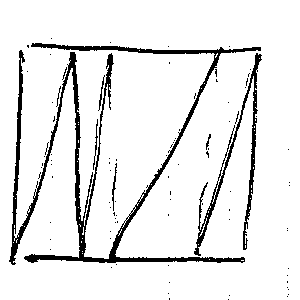
\includegraphics[width=\linewidth]{figures/gelfand-0154-p001416-interval-graph-original.png}\par\smallskip
{\footnotesize Original manuscript detail: \texttt{GELFAND-P001416}}
\end{minipage}\hfill
\begin{minipage}[t]{.50\linewidth}\vspace{0pt}\centering
{\footnotesize Partial visible-stroke recreation}\par\smallskip
\resizebox{\linewidth}{!}{% Visible strokes only. Coordinate scale reproduces the sketch, not an exact map.
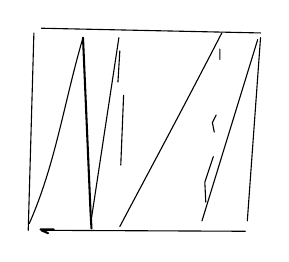
\begin{tikzpicture}[x=.012cm,y=-.012cm,line cap=round]
\draw (20,50)--(14,259) (28,45)--(260,50) (260,55)--(246,249)
 (31,259)--(244,260);
\draw (15,252) .. controls (43,189) and (52,123) .. (72,55);
\draw[line width=.75pt] (72,55)--(80,240)--(81,257);
\draw (81,246)--(110,55);
\draw (111,69)--(109,102) (115,116)--(112,190);
\draw (111,255) .. controls (140,200) and (171,143) .. (219,50);
\draw (198,249)--(257,57);
\draw (202,229)--(201,208)--(210,181) (211,155)--(209,145)--(213,137)
 (217,67)--(217,78);
% The thick bottom-left terminal trace is not interpreted as an arrow.
\draw[line width=.75pt] (27,258)--(41,258) (28,259)--(35,262);
\end{tikzpicture}
}
\end{minipage}
\end{center}
\noindent{\small\textit{Open joins and short vertical traces remain unresolved after 3×, 5× and 10× inspection. Plain strokes do not specify arrows, discontinuities or extra axis values.}}


\begin{equation}
 \zeta_T(z,\varphi)=\frac{\det(1-zL_1)}{\det(1-zL_2)},
 \tag{1}
\end{equation}
where
\begin{equation*}
 L_1f(z)=\varphi(z)\sum\frac{1}{\rho_j}f(\psi_j(z)),
\end{equation*}
\begin{equation*}
 L_2f(z)=\varphi(z)\sum f(\psi_j(z)),
\end{equation*}
$\psi_j$ are local inverses of $T$ on the interval $I_j$, and $\rho_j^{-1}$ is the slope.
\EnglishUnclear{GELFAND-P001416}{slope-letter}{The letter in $\rho_j$ also admits the reading $p_j$.}

In the general case:
\begin{equation}
 \zeta_T(z,\varphi)=
 \exp\left(
 \sum_{n=1}^{\infty}\frac{z^n}{n}
 \sum_{\xi\in\mathrm{Fix}\,T^n}
 \prod_{k=0}^{n-1}\varphi(T^k x)
 \right)
 \tag{2}
\end{equation}
\EnglishUnclear{GELFAND-P001416}{eq2-variable}{Below the second sum is written $\xi\in\mathrm{Fix}\,T^n$; in the product, $x$.}


\EnglishSourceFrame{GELFAND-P001417}{unlabelled}
\underline{7/XII-87.}\qquad \underline{Gelfand seminar!}\qquad Something on the paper by

\underline{D. Mayer}\qquad \underline{Lett. in Math. Phys. 1987, $14:2$}

\underline{On the Ruelle $\zeta$ function}

$F$ is the set of spin values (finite).

We study spin configurations on a lattice
\begin{equation*}
 (\xi_i),\qquad -\infty<i<\infty,\qquad \xi_i\in F.
\end{equation*}
$M\subseteq F\times F$ is the admissible set; we require
\begin{equation}
 (\xi_i,\xi_{i+1})\in M.
 \tag{1}
\end{equation}

The simplest example of a Ruelle $\zeta$ function is the Artin–Mazur $\zeta$ function.

Consider the set of periodic configurations and their number:
\begin{equation}
 N_n=\#\{(\xi_i)\mid\mathcal T^n(\xi_i)=(\xi_i)\}
 =\mathrm{Fix}\,\mathcal T^n,
 \tag{2}
\end{equation}
where $\mathcal T$ is the transformation in the sequence space
\begin{equation*}
 \mathcal T(\xi_i)=\xi_{i+1}
\end{equation*}
(shift)

The Ruelle $\zeta$ function:
\begin{equation}
 \zeta_{\mathcal T}(s)=\exp\left(\sum_{n=1}^{\infty}\frac{N_n}{n}s^n\right)
 \tag{3}
\end{equation}
the series converges for $|s|<\dfrac{1}{|F|}$.

\EnglishUnclear{GELFAND-P001417}{continuation-question-overwriting}{Does analytic continuation exist? [The end of the source abbreviation “Sushch.” and the initial “a” are retraced over earlier strokes.]}
Consider the matrix
\begin{equation}
 T=(T_{\alpha\beta})=
 \begin{cases}
 1,&(\alpha,\beta)\in M,\\
 0,&(\alpha,\beta)\notin M.
 \end{cases}
 \tag{4}
\end{equation}

Then
\begin{equation}
 \zeta_{\mathcal T}(s)=\frac{1}{\det(1-sT)}
 \tag{5}
\end{equation}

It follows that $\zeta_{\mathcal T}(s)$ is meromorphic.

The radius of convergence may exceed $1/|F|$.

For the proof, note that
\begin{equation}
 N_n=\mathrm{Tr}\,T^n.
 \tag{6}
\end{equation}


\EnglishSourceFrame{GELFAND-P001418}{62}
\underline{Remark by I. M. G.}: this resembles the work of Dynkin and Dmitriev:
consider a stoch. matrix $(p_{ik})$ [inserted above: (stochastic)]
(in the problem of reservoirs, this is
[crossed-out sign: \EnglishUnclear{GELFAND-P001418}{basin-cancelled-sign}{illegible}]
the fraction of water flowing from reservoir $i$ into reservoir $k$).
\begin{equation*}
 \underline{P}=(p_{ik}),\qquad \sum_k p_{ik}=1.
\end{equation*}
This depends on the eigenvalues of $P$.

a) The eigenvalues lie in the disk $|\lambda|\leq1$,

b) $1$ is an eigenvalue.

What region do the eigenvalues fill?

It is the interior of some algebraic curve.

They did it incorrectly.

There is a family of eigenvalues!!

and one should draw the family of eigenvalues in $\mathbb C^n$---it should
be a beautiful region (\underline{Problem!!})

Projection onto one axis may be complicated!

[A double line on the left; the following two lines are underlined:]
\underline{In the Ruelle problem, it is interesting to examine all eigenvalues}

\underline{of the matrix $T$.}

\medskip
\underline{Speaker}. Generalisation of example (3)
\begin{equation}
 \zeta_{\mathcal T}(s;\varphi)=
 \exp\left(
 \sum_{n=1}^{\infty}\frac{s^n}{n}
 \sum_{\xi\in\mathrm{Fix}(\mathcal T^n)}
 \prod_{\ell=0}^{n}\varphi(\mathcal T^\ell\xi)
 \right)
 \tag{7}
\end{equation}
\EnglishUnclear{GELFAND-P001418}{eq7-upper-product-bound}{The upper product limit is written as $n$.}

Here
\begin{equation*}
 \varphi=\varphi(\xi_1,\ldots,\xi_k),\qquad \xi_j\in F
\end{equation*}
[Below $\varphi$, a line leads to the caption: function.]

($\varphi$ depends only on the first $k$ values).

((3) is obtained for $\varphi=1$)

(8) \underline{Assertion.} $\exists$ [crossed out: operator; inserted above the line: matrix]
$L$ (finite-dimensional), such that:
\begin{equation}
 \zeta_{\mathcal T}(s,\varphi)=\frac{1}{\det(1-sL)}
 \tag{9}
\end{equation}

Specifically, consider
\begin{equation*}
 F'=F^k;
\end{equation*}
[Crossed out: \EnglishUnclear{GELFAND-P001418}{before-m-prime-cancelled}{an illegible entry before $M'$}.]
\begin{equation*}
 M'\subset F'\times F'
\end{equation*}
\begin{equation}
 M'=\{(\xi_1,\ldots,\xi_k);(\xi_2,\ldots,\xi_{k+1})
 \mid(\xi_i,\xi_{i+1})\in M\}
 \tag{10}
\end{equation}
\EnglishUnclear{GELFAND-P001418}{eq10-overwritten-indices}{In the second tuple, the indices $2$ and $k+1$ are corrected; in the condition, $i+1$ is also retraced.}

Then take
\begin{equation*}
 \ell_{\alpha\beta}=
 \begin{cases}
 \varphi(\alpha),&(\alpha,\beta)\in M',\\
 0,&(\alpha,\beta)\notin M',
 \end{cases}
 \qquad L=(\ell_{\alpha\beta}).
\end{equation*}


\EnglishSourceFrame{GELFAND-P001419}{unlabelled}
\underline{I. M. G.:}

\underline{NB}: one must know the $p$-adic numbers

(be able to add, multiply and divide them,
[crossed out: \EnglishUnclear{GELFAND-P001419}{nb-cancelled-letter}{an illegible sign}]
extract roots!)

\medskip
\underline{A. Beilinson}\qquad
\underline{$p$-adic numbers and physics.}

\underline{On some of Manin's $p$-adic ideas in physics}
\EnglishUnclear{GELFAND-P001419}{heading-last-sign}{!; possibly ?}

$1^{\circ}$. Witten listened to a talk by
\EnglishUnclear{GELFAND-P001419}{faltings-name}{Faltins [source candidate]}
with great interest, after which he bought all the books on number theory.
The only thing he understood from the talk was the formula
\begin{equation}
 |a|_\infty\cdot|a|_2|a|_3\ldots=1,\qquad a\in\mathbb Q.
 \tag{1}
\end{equation}
For $\dfrac12$, this reads:
\begin{equation*}
 \frac12\cdot2\cdot1\ldots=1.
\end{equation*}

There are three papers:

1) \underline{Volovich}\qquad (in Russian)

2) \underline{Yu. I. Manin}\qquad (in English)

3) \underline{Witten} and someone else
\EnglishUnclear{GELFAND-P001419}{witten-list-final-sign}{[an illegible separate sign after the line]}

All three papers appeared in September.

\underline{Witten's text.}

Consider the functional equation for the Riemann $\zeta$ function
\begin{equation}
 \pi^{-s/2}\Gamma(s/2)\prod(1-p^{-s})^{-1}
 =
 \pi^{-(1-s)/2}\Gamma\left(\frac{1-s}{2}\right)
 \prod(1-p^{-(1-s)})^{-1}.
 \tag{2}
\end{equation}
(analytic continuation is understood)

or (formally):
\begin{equation}
 \frac{\pi^{-s+1}\Gamma(s/2)}
 {\Gamma\left(\dfrac{1-s}{2}\right)}
 =
 \prod_p\frac{1-p^{-s}}{1-p^{s-1}}.
 \tag{3}
\end{equation}
\EnglishUnclear{GELFAND-P001419}{eq3-pi-exponent}{The exponent of $\pi$ is written as $-s+1$.}

On the left is $\approx$ the Veneziano–Witten amplitude for an open
string [inserted above: (with momentum $s$)].
On the right is a divergent expression, but what matters is
that it is represented as a product over the primes!


\EnglishSourceFrame{GELFAND-P001420}{63}
\underline{$2^{\circ}$. On Manin's work}

(1) \underline{Assertion}: The Tamagawa measure $=1$.

In more detail:
\begin{equation*}
 \mathrm{SL}(n,\mathbb R)\supset\mathrm{SL}(n,\mathbb Z).
\end{equation*}
On $\mathrm{SL}(n,\mathbb R)$ there is an invariant measure (standard)
[above “invariant”, inserted: left].

Normalise [crossed out:
\EnglishUnclear{GELFAND-P001420}{normalization-cancelled}{illegible}]
using the integer matrices.
\begin{equation*}
 \operatorname{vol}\bigl(\mathrm{SL}(n,\mathbb R)/\mathrm{SL}(n,\mathbb Z)\bigr)-?
\end{equation*}

[In the right margin:]
\par\nopagebreak[4]
(constructed using the standard basis in the Lie algebra
$\mathfrak{sl}(n,\mathbb R)$ or in $\mathfrak{gl}(n,\mathbb R)$
[crossed out: \EnglishUnclear{GELFAND-P001420}{margin-cancelled}{an illegible sign}]
standard basis;
\begin{center}
 \fbox{$\operatorname{vol}_{sl}=\dfrac{\operatorname{vol}_{gl}}{d\,\operatorname{tr}}$}
\end{center}
\EnglishUnclear{GELFAND-P001420}{margin-volume-formula}{The marginal formula: $\operatorname{vol}_{sl}=\operatorname{vol}_{gl}/d\,\operatorname{tr}$; the small letters beside $\operatorname{vol}$ require checking.}

$\mathrm{SL}(2,\mathbb R)$ consists of conformal transformations of the unit disk, acting transitively
on $S^*H^2$.

The invariant volume on $S^*H^2$ is
[crossed out: \EnglishUnclear{GELFAND-P001420}{invariant-volume-cancelled}{an illegible sign}]
$\operatorname{vol}_{H^2}\otimes d\varphi$.

\begin{center}
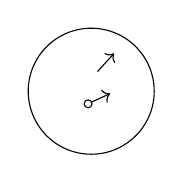
\begin{tikzpicture}[x=1cm,y=1cm]
 \draw (0,0) circle (0.8);
 \draw (-0.04,-0.16) circle (0.05);
 \draw[->] (0,-0.14) -- (0.24,-0.03);
 \draw[->] (0.08,0.25) -- (0.29,0.48);
\end{tikzpicture}
\end{center}

Or: quotient by the maximal compact subgroup

\begin{center}
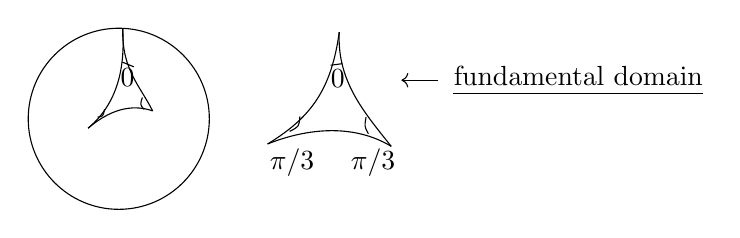
\begin{tikzpicture}[x=1cm,y=1cm]
 \draw (0,0) circle (1.15);
 \draw (0.05,1.14) .. controls (0.08,0.65) and (-0.01,0.2) .. (-0.39,-0.12);
 \draw (0.05,1.14) .. controls (0.04,0.62) and (0.27,0.42) .. (0.43,0.10);
 \draw (-0.39,-0.12) .. controls (-0.05,0.17) and (0.23,0.17) .. (0.43,0.10);
 \draw (0.045,0.72) -- (0.19,0.66);
 \draw (-0.27,0.02) .. controls (-0.2,0.03) .. (-0.18,0.12);
 \draw (0.32,0.12) .. controls (0.27,0.18) .. (0.30,0.27);
 \node at (0.11,0.52) {$0$};
 \draw (2.8,1.1) .. controls (2.7,0.38) and (2.45,0.02) .. (1.89,-0.32);
 \draw (2.8,1.1) .. controls (2.77,0.48) and (3.11,0.09) .. (3.46,-0.35);
 \draw (1.89,-0.32) .. controls (2.39,-0.12) and (2.98,-0.06) .. (3.46,-0.35);
 \draw (2.69,0.68) -- (2.84,0.7);
 \draw (2.17,-0.16) .. controls (2.29,-0.1) .. (2.30,0.03);
 \draw (3.17,-0.19) .. controls (3.12,-0.10) .. (3.14,0.02);
 \node at (2.78,0.51) {$0$};
 \node at (2.20,-0.55) {$\pi/3$};
 \node at (3.23,-0.55) {$\pi/3$};
 \draw[->] (4.05,0.49) -- (3.59,0.49);
 \node[anchor=west] at (4.13,0.49) {\underline{fundamental domain}};
\end{tikzpicture}
\end{center}

\underline{Answer.}
\begin{equation}
 \operatorname{vol}\mathrm{SL}(n,\mathbb R)/\mathrm{SL}(n,\mathbb Z)
 =\zeta(2)\zeta(3)\ldots\zeta(n)
 \tag{2}
\end{equation}
$\mathbb A$ denotes the adeles;
\begin{equation}
 \begin{gathered}
 \mathrm{SL}(n,\mathbb A)\sim
 \mathrm{SL}(n,\mathbb R)\times\mathrm{SL}(n,\mathbb Q_2)\times\ldots\\
 \cup\\
 \mathrm{SL}(n,\mathbb Q)
 \end{gathered}
 \tag{3}
\end{equation}
\begin{equation}
 \operatorname{vol}\mathrm{SL}(n,\mathbb A)/\mathrm{SL}(n,\mathbb Q)=1.
 \tag{4}
\end{equation}
\begin{equation*}
 \operatorname{vol}\mathrm{SL}(n,\mathbb A)/\mathrm{SL}(n,\mathbb Q)
 \sim
 \operatorname{vol}\mathrm{SL}(n,\mathbb R)/\mathrm{SL}(n,\mathbb Z)
 \prod\operatorname{vol}\mathrm{SL}(n,\mathbb Z_p).
\end{equation*}
\begin{equation}
 \operatorname{vol}\mathrm{SL}(n,\mathbb Z_p)
 \sim\#\mathrm{SL}_n(\mathbb F_p)/p^{n^2-1}.
 \tag{5}
\end{equation}
\underline{Exercise}: calculate $\#\mathrm{SL}_n(\mathbb F_p)$.


\EnglishSourceFrame{GELFAND-P001421}{unlabelled}
(6) The number of elements of $\mathrm{GL}(n,\mathbb F_p)$
\begin{equation*}
 (p^n-1)(p^n-p)(p^n-p^2)\ldots
 =
 p^{n^2}(1-p^{-n})(1-p^{-n+1})\ldots(1-p^{-1}).
\end{equation*}

(7) For $\mathrm{SL}(n,\mathbb F_p)$, divide by $p-1$:
\begin{equation*}
 p^{n^2-1}(1-p^{-n})(1-p^{-n+1})\ldots(1-p^{-2}).
\end{equation*}
This is a product of Euler factors.

(8) \underline{Conjecture of Yu. I. Manin}: an analogue of formula (2) can be written for
the moduli spaces of curves arising in string theory.

\underline{I. M. G.}

\underline{Mathematical question}: the volume of Teichmüller space has a $p$-adic analogue.

Or: what is adelic Teichmüller space

\medskip
\underline{An example of the \EnglishUnclear{GELFAND-P001421}{witten-heading-faint-word}{power} of Witten's work:}

\underline{Laumon} produced a work in number theory based on Witten's ideas
from Morse theory.

Idea: consider a function $u\in\mathcal E'(\mathbb R)$,
$\widetilde u(\xi)\in C^\infty$
and all singularities will move into the asymptotics at infinity.

\underline{Advice from I. M. G.}: read Kharkevich's book
“Spectra, [crossed out:
\EnglishUnclear{GELFAND-P001421}{book-title-cancelled}{illegible};
inserted above the line: signals] and noise”,
to understand the \underline{Fourier transform}.

On the work of \underline{Laumon}.

\begin{center}
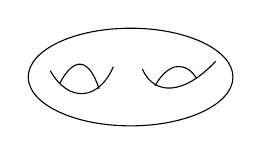
\begin{tikzpicture}[x=1cm,y=1cm]
 \draw (0,0) ellipse (1.3 and 0.62);
 \draw (-1.02,0.08) .. controls (-0.78,-0.34) and (-0.40,-0.29) .. (-0.22,0.13);
 \draw (-0.90,-0.08) .. controls (-0.72,0.26) and (-0.53,0.25) .. (-0.40,-0.15);
 \draw (0.15,0.10) .. controls (0.30,-0.24) and (0.68,-0.23) .. (1.08,0.20);
 \draw (0.31,-0.11) .. controls (0.50,0.22) and (0.72,0.18) .. (0.84,-0.02);
\end{tikzpicture}
\end{center}

Consider the surface $\mathcal F$
\begin{equation*}
 H^i(X,\mathcal F),\qquad i=0,1,2.
\end{equation*}
\EnglishUnclear{GELFAND-P001421}{surface-symbol}{After “surface” is written $\mathcal F$; subsequently, $H^i(X,\mathcal F)$.}

\begin{equation}
 \det H^\bullet(X,\mathcal F)=
 \frac{\det H^0(X,\mathcal F)\det H^2(X,\mathcal F)}
 {\det H^1(X,\mathcal F)\;
 \text{[crossed out: }\det H^2(X,\mathcal F)\text{]}}
 \tag{1}
\end{equation}
([Crossed out:
\EnglishUnclear{GELFAND-P001421}{before-vector-spaces-cancelled}{finite?}]
vector spaces;
$\det$ is the highest exterior power)

Automorphisms?

Consider a triangulation; $\det H^\bullet$ is identified with the product of the $\det$
of the terms of the complex (an Euler-type formula): canonically


\EnglishSourceFrame{GELFAND-P001422}{64}
\begin{equation*}
\det(C^\bullet)=\det(H^\bullet(C)) \tag{2}
\end{equation*}
$2-2g$ is the Euler characteristic.

On the other hand
\begin{equation*}
2g-2=\operatorname{deg}K
\end{equation*}
[Below $K$: “canonical class”.]

\underline{Let}

$D$ be a divisor;
\begin{equation*}
\det\mathcal F_D=\bigotimes(\det\mathcal F_{x_i})^{\otimes a_i},
\qquad D=\sum a_i x_i \tag{3}
\end{equation*}
[Crossed out:
\EnglishUnclear{GELFAND-P001422}{cancelled-divisor-map}{$D\to D+K$ or $D\mapsto D+K$; reading not established}.]

\underline{Deligne's formula:}
\begin{equation*}
\det H^\bullet=\det\mathcal F_K \tag{4}
\end{equation*}
[A separate sign on the right is crossed out:
\EnglishUnclear{GELFAND-P001422}{eq4-cancelled-sign}{illegible}.]
\EnglishUnclear{GELFAND-P001422}{eq4-determinant-convention}{In (4), $\det H^\bullet=\det\mathcal F_K$ is written without an exponent $-1$.}

(fix a complex structure and a choice of point in the canonical class)

For an arbitrary constructible sheaf, $\underline{\det}$ is also defined, and
there is an analogue of Deligne's formula!

Here functions with singularities arise on $\mathbb A^1$

\underline{\underline{Klyachko.}}\quad
\underline{\underline{Toric bundles.}}

A toric variety is a variety $X$ on which an algebraic torus $T$ acts;
there is an orbit isomorphic to $T$.
\begin{equation*}
X=\bigcup_\sigma O_\sigma,\quad\text{--- decomposition into orbits}
\end{equation*}
$\mathcal E$ is a bundle on $X$ with a toric structure
(and the action lifts! The diagram
\begin{equation*}
\begin{tikzcd}
\mathcal E \arrow[r,"t"] \arrow[d] & \mathcal E \arrow[d] \\
X \arrow[r,"t"] & X
\end{tikzcd}
\end{equation*}
commutes)

One can describe the moduli of [inserted above the line: “such”]
bundles in the language of linear algebra.


\EnglishSourceFrame{GELFAND-P001423}{unlabelled}
The structure of $X$ is described by a fan $\Sigma$ in the Lie algebra of the torus.
\begin{center}
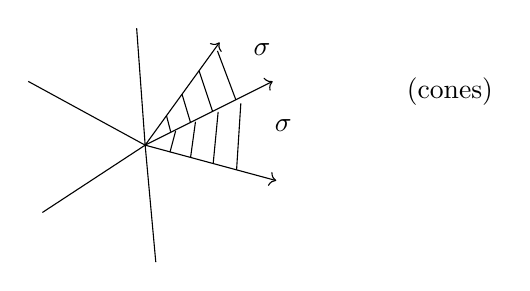
\begin{tikzpicture}[scale=0.9]
\draw (0,0) -- (-1.65,0.9);
\draw (0,0) -- (-1.45,-0.95);
\draw (0,0) -- (-0.12,1.65);
\draw (0,0) -- (0.15,-1.65);
\draw[->] (0,0) -- (1.05,1.45);
\draw[->] (0,0) -- (1.8,0.9);
\draw[->] (0,0) -- (1.85,-0.5);
\draw (0.36,0.19) -- (0.3,0.42);
\draw (0.64,0.32) -- (0.52,0.72);
\draw (0.95,0.48) -- (0.76,1.05);
\draw (1.28,0.64) -- (1.02,1.33);
\draw (0.35,-0.10) -- (0.43,0.20);
\draw (0.64,-0.18) -- (0.71,0.33);
\draw (0.96,-0.26) -- (1.03,0.47);
\draw (1.29,-0.35) -- (1.35,0.59);
\node at (1.65,1.35) {$\sigma$};
\node at (1.95,0.28) {$\sigma$};
\node at (4.3,0.75) {(cones)};
\end{tikzpicture}
\end{center}
$|\Sigma|$ is the set of $1$-dimensional cones of the fan $\Sigma$.

\underline{Theorem.}
(category of toric bundles) $\Longleftrightarrow$
(category of vector spaces
[crossed-out sign:
\EnglishUnclear{GELFAND-P001423}{theorem-cancelled-sign}{illegible}]
$E$ with a family [inserted above the line: “decreasing $\mathbb Z$-”]
of filtrations $E^\alpha(i)$, $\alpha\in|\Sigma|$, satisfying the condition

A) The filtrations $E^\alpha$, $\alpha\in\sigma\in\Sigma$,
are distributive.

\underline{Problems.}
1) Describe the geometry of the bundle (cohomology, characteristic classes
and so on) in terms of the filtrations

2) classification---?

Let $\Sigma$ be a simplicial complex; associate a filtration
to each vertex

A representation of it is a family of filtrations in a vector space
[inserted above the line: «$E$:»] $E^\alpha(i)$,
$\alpha\in$ [crossed-out sign:
\EnglishUnclear{GELFAND-P001423}{representation-cancelled-sign}{illegible}]
$\Sigma$,
\begin{equation*}
E\ldots\supset E^\alpha(i)\supset E^\alpha(i+1)\supset\ldots 0
\end{equation*}
\begin{equation*}
\alpha\in(\text{vertices of the complex})=\Sigma.
\end{equation*}
The spaces $E^\alpha(i)$, $\alpha\in\sigma$, are distributive for fixed $\sigma$
(for all $i$)

[Below the first $\sigma$: “simplex”. A framed insertion:]
(i.e. generate a distributive lattice)

For example, if

$\alpha_1,\alpha_2,\alpha_3$ are the vertices of a triangle $\Delta$, then

$E^{\alpha_1}\quad E^{\alpha_2}\quad E^{\alpha_3}$ are distributive, i.e.
\begin{equation*}
(E^{\alpha_1}+E^{\alpha_2})\cap E^{\alpha_3}
=E^{\alpha_1}\cap E^{\alpha_3}+E^{\alpha_2}\cap E^{\alpha_3}
\end{equation*}

\underline{Classify:} a good problem

For a triangle: it is solved trivially

For the surface of a tetrahedron $\Sigma=\partial\Delta$, where $\Delta$ is a simplex, the answer
is as follows: in [crossed out:
\EnglishUnclear{GELFAND-P001423}{tetrahedron-cancelled-space}{$\mathbb R^3$-space; reading not established}]
$E$, $\dim E=3$, consider $4$ $2$-dimensional subspaces in general position.
\begin{equation*}
\mathcal E=(E;\ E^\alpha,E^\beta,E^\gamma,E^\delta)
\end{equation*}


\EnglishSourceFrame{GELFAND-P001424}{65}
one must also take the exterior powers
\begin{equation*}
\Lambda^i\mathcal E=
(\Lambda^i E,\Lambda^i E^\alpha,\Lambda^i E^\beta,
\Lambda^i E^\gamma,\Lambda^i E^\delta)
\end{equation*}
A general representation decomposes into a direct sum of $1$-dimensional ones and these.

\underline{I. M. G.}
The right problem: isolate solvable parts in $\forall$ problem
(the Gelf.–Ponomarev approach)

V. [a corrected and crossed-out initial:
\EnglishUnclear{GELFAND-P001424}{kac-initial}{illegible}]
\underline{Kac} describes all this in the language of graphs and
\underline{Kac–Moody algebras}:
the dimensions at the vertices = coordinates of roots, and so on.

The number of parameters is found.

Lect. Notes, \underline{996}; an earlier paper — \underline{Inventiones}.

(a conference talk)

[A line is crossed out:
\EnglishUnclear{GELFAND-P001424}{cancelled-seminar-line}{Seminar \ldots; the rest is illegible}.]

\EnglishIncomplete{GELFAND-P001424}{cancelled-seminar-content}{A full reading of the crossed-out line before “Next time: 8 February” has not been established; the possible initial word is given above.}

\underline{Next time:}\quad \underline{8 February.}


\clearpage\section*{Complete reading notes}
\subsection*{\texttt{GELFAND-P001385}}
\par\noindent\leavevmode\phantomsection\label{GELFAND-0151-U001}\label{GELFAND-P001385:cancelled-upper:note}\textbf{\texttt{GELFAND-0151-U001}}.\nopagebreak[4]\par
In item4, between "Combinatorial" and "sheaves", one word is crossed out repeatedly; parts of the initial letters and ending can be distinguished.\par
Candidates: constructible. Unresolved in the diplomatic source.\par
Historical source review: original-pixel coordinates [590,800,1170,935],3x enlargement. The candidate is not asserted; the cancellation is retained.\par\medskip
\par\noindent\leavevmode\phantomsection\label{GELFAND-0151-U002}\label{GELFAND-P001385:lower-gluing:note}\textbf{\texttt{GELFAND-0151-U002}}.\nopagebreak[4]\par
In the line "There is an identification of sections, ...", the last word is abbreviated; its initial "is" is readable, followed by merged strokes and a period.\par
Candidates: iskhod. [source: «исход.»; unexpanded]; iskhd. [source: «исхд.»; unexpanded]. Unresolved in the diplomatic source.\par
Historical source review: coordinates [850,3000,2160,3180],3x. The next line reads "from different families". The abbreviation has not been expanded.\par\medskip
\par\noindent\leavevmode\phantomsection\label{GELFAND-0151-U003}\label{GELFAND-P001385:cancelled-bottom:note}\textbf{\texttt{GELFAND-0151-U003}}.\nopagebreak[4]\par
Between "C\textasciicircum{}+ is" and "the sheaf", a small word or beginning of a word is crossed out with several lines.\par
Candidates: this [source: «это»]; pred... [unresolved source beginning: «пред...»]. Unresolved in the diplomatic source.\par
Historical source review: coordinates [435,3240,635,3360],5x. The actual cancelled reading has not been established.\par\medskip
\subsection*{\texttt{GELFAND-P001386}}
\par\noindent\leavevmode\phantomsection\label{GELFAND-0151-U004}\label{GELFAND-P001386:cancelled-exercise:note}\textbf{\texttt{GELFAND-0151-U004}}.\nopagebreak[4]\par
In exercise1, before "Construct C\textasciicircum{}+", a short beginning of a word is crossed out; a descending stroke and loop are visible.\par
Candidates: pro... [unresolved source beginning: «про...»]. Unresolved in the diplomatic source.\par
Historical source review: coordinates [610,905,760,1030],4x. The complete cancelled word has not been established.\par\medskip
\par\noindent\leavevmode\phantomsection\label{GELFAND-0151-U005}\label{GELFAND-P001386:path-diagram:note}\textbf{\texttt{GELFAND-0151-U005}}.\nopagebreak[4]\par
Two ovals V\_1 and V\_2, points inside, and a wavy line joining them. The lower letters have S-shaped forms with subscripts1 and2.\par
Candidates: s\_1, s\_2; xi\_1, xi\_2. Unresolved in the diplomatic source.\par
Historical source review: coordinates [315,2460,870,2760],4x. The geometry is visible, but the lower letter labels have not been determined uniquely. No direction of transport or arrows indistinguishable in the source have been added.\par\medskip
\subsection*{\texttt{GELFAND-P001387}}
\par\noindent\leavevmode\phantomsection\label{GELFAND-0151-U006}\label{GELFAND-P001387:cancelled-pullback:note}\textbf{\texttt{GELFAND-0151-U006}}.\nopagebreak[4]\par
In the assertion, after "inverse image", a word resembling the source plural "sheaves" is crossed out, followed by the clearly written "a sheaf on Gamma".\par
Candidates: sheaves [source genitive plural: «пучков»]. Unresolved in the diplomatic source.\par
Historical source review: coordinates [1800,475,2040,552],4x. The middle letters are obscured by horizontal lines; the candidate remains unresolved.\par\medskip
\subsection*{\texttt{GELFAND-P001388}}
\par\noindent\leavevmode\phantomsection\label{GELFAND-0151-U007}\label{GELFAND-P001388:dual-note:note}\textbf{\texttt{GELFAND-0151-U007}}.\nopagebreak[4]\par
In parentheses to the right of the definition of the dual presheaf, "analogue of raspredeleni..." is written; the ending of the final word is faint.\par
Candidates: distributions [source genitive plural: «распределений»]; a distribution [source singular ending: «распределения»]. Unresolved in the diplomatic source.\par
Historical source review: coordinates [810,320,2040,510],3x. The remaining explanatory parenthesis below reads "the dual space in the sense of linear algebra".\par\medskip
\subsection*{\texttt{GELFAND-P001389}}
\par\noindent\leavevmode\phantomsection\label{GELFAND-0151-U008}\label{GELFAND-P001389:author-name:note}\textbf{\texttt{GELFAND-0151-U008}}.\nopagebreak[4]\par
In the line "In1970, J. Math. Phys., a proof by ... in two lines", the first letter of the surname has a large upper loop and lower bend; the visible reading is closer to «Вуда» (Vuda, rendered Wood).\par
Candidates: Wood [source candidate: «Вуда»]; Good [source candidate: «Гуда»]. Unresolved in the diplomatic source.\par
Historical source review: coordinates [990,2710,1185,2810],6x; the line was also checked in [170,2590,1700,2810] at3x. The surname was not replaced by the name expected from the known proof; no external bibliographical verification was performed.\par\medskip
\par\noindent\leavevmode\phantomsection\label{GELFAND-0151-U009}\label{GELFAND-P001389:interpolation-function:note}\textbf{\texttt{GELFAND-0151-U009}}.\nopagebreak[4]\par
Before the substitution x=0, the manuscript clearly writes f identically0; the next formula(3) has1 on the right.\par
Candidates: f identically0: the visible writing. Unresolved in the diplomatic source.\par
Historical source review: coordinates [1725,2820,1950,2930],6x. Mathematical comparison: interpolation of the identically zero function does not produce the right-hand side1; the constant function1 is normally needed. This is an observation about a possible source error, not grounds for correcting the visible zero. The formula is reproduced without replacement.\par\medskip
\subsection*{\texttt{GELFAND-P001390}}
\par\noindent\leavevmode\phantomsection\label{GELFAND-0151-U010}\label{GELFAND-P001390:cancelled-let:note}\textbf{\texttt{GELFAND-0151-U010}}.\nopagebreak[4]\par
Before "Let G(a)", a small vertical fragment is crossed out repeatedly; it may be the beginning of the Cyrillic letter P.\par
Candidates: P... [source Cyrillic «П...»]. Unresolved in the diplomatic source.\par
Historical source review: coordinates [310,255,390,358],6x. The word is not reconstructed from the meaning of the following phrase.\par\medskip
\par\noindent\leavevmode\phantomsection\label{GELFAND-0151-U011}\label{GELFAND-P001390:cancelled-neumann:note}\textbf{\texttt{GELFAND-0151-U011}}.\nopagebreak[4]\par
In the right column, before the surviving "C. Neumann", another writing of the name is crossed out; C. and the beginning N/Ne can be distinguished.\par
Candidates: C. Neu...; C. Neumann. Unresolved in the diplomatic source.\par
Historical source review: coordinates [1590,1670,1810,1760],5x. The remaining letters are obscured by several lines.\par\medskip
\par\noindent\leavevmode\phantomsection\label{GELFAND-0151-U012}\label{GELFAND-P001390:equation-end:note}\textbf{\texttt{GELFAND-0151-U012}}.\nopagebreak[4]\par
To the right of the coordinate equation(1-double-prime), an isolated crossed-out sign has a loop and a descending stroke.\par
Candidates: q; u. Unresolved in the diplomatic source.\par
Historical source review: coordinates [1800,2350,1940,2450],5x. It is unclear whether this is a cancelled continuation symbol for the formula or a pen trial; the sign is recorded but not inserted into the equation.\par\medskip
\par\noindent\leavevmode\phantomsection\label{GELFAND-0151-U013}\label{GELFAND-P001390:constants-note:note}\textbf{\texttt{GELFAND-0151-U013}}.\nopagebreak[4]\par
Beneath lambda and v in the addition about changing the parameter are pairs of short vertical strokes; const is written twice, further below.\par
Candidates: a vertical equality; strokes pointing to the word const. Unresolved in the diplomatic source.\par
Historical source review: coordinates [1700,2560,2180,2740],4x. The meaning of the strokes has not been established. They cannot silently be converted into lambda=const, lambda not equal to const, or corresponding assertions for v; the text gives a literal description of their placement.\par\medskip
\par\noindent\leavevmode\phantomsection\label{GELFAND-0151-U014}\label{GELFAND-P001390:bijection-note:note}\textbf{\texttt{GELFAND-0151-U014}}.\nopagebreak[4]\par
After "takes solutions of problem1) to solutions of problem2)", parentheses read "and vzaimo..."; the ending is abbreviated and the letters merged.\par
Candidates: vzaimoodn. [source: «взаимоодн.»; unexpanded]; vzaimodn. [source: «взаимодн.»; unexpanded]. Unresolved in the diplomatic source.\par
Historical source review: coordinates [1080,2810,2200,3020],3x. The line below reads "H. Knorrer,1982". The abbreviation has not been expanded into a complete assertion of bijectivity.\par\medskip
\subsection*{\texttt{GELFAND-P001391}}
\subsection*{\texttt{GELFAND-P001392}}
\par\noindent\leavevmode\phantomsection\label{GELFAND-0151-U015}\label{GELFAND-P001392:cancelled-equivalence:note}\textbf{\texttt{GELFAND-0151-U015}}.\nopagebreak[4]\par
After the equivalence sign and before "combinatorial sheaves", a word is crossed out; parts of "kon..." and descending middle strokes are visible.\par
Candidates: constructible. Unresolved in the diplomatic source.\par
Historical source review: coordinates [1700,157,1988,259],4x. The middle and ending are heavily obscured by lines; the candidate is not asserted.\par\medskip
\par\noindent\leavevmode\phantomsection\label{GELFAND-0151-U016}\label{GELFAND-P001392:objects-mark:note}\textbf{\texttt{GELFAND-0151-U016}}.\nopagebreak[4]\par
Between "Objects" and "C(A)", a small cluster of strokes has a transverse line and loops; it may be a crossed-out word or a symbol.\par
Candidates: crossed-out "from" [source: «из»]; a membership sign. Unresolved in the diplomatic source.\par
Historical source review: coordinates [570,1100,660,1200],6x. It was not silently converted into either an ordinary "from" or the mathematical membership sign.\par\medskip
\subsection*{\texttt{GELFAND-P001393}}
\par\noindent\leavevmode\phantomsection\label{GELFAND-0151-U017}\label{GELFAND-P001393:cancelled-left:note}\textbf{\texttt{GELFAND-0151-U017}}.\nopagebreak[4]\par
To the left of the lower half of the diamond-shaped diagram, a short phrase is crossed out: "v", "k", the descending stroke of r and a mark above the ending can be seen.\par
Candidates: in which [source abbreviation: «в к-рой»]. Unresolved in the diplomatic source.\par
Historical source review: coordinates [240,2845,490,2970],5x. It probably repeats the phrase in the next line, but the crossed-out middle and final strokes do not provide an independent confident reading. The candidate remains unresolved.\par\medskip
\subsection*{\texttt{GELFAND-P001394}}
\par\noindent\leavevmode\phantomsection\label{GELFAND-0151-U018}\label{GELFAND-P001394:elementary-abbrev:note}\textbf{\texttt{GELFAND-0151-U018}}.\nopagebreak[4]\par
In the line "under the equivalence relation generated by the ... relation", an abbreviation precedes the last word: e, l, m and a period are clear; a separate e between l and m is not established.\par
Candidates: elm. [source: «элм.»; unexpanded]; elem. [source: «элем.»; unexpanded]. Unresolved in the diplomatic source.\par
Historical source review: coordinates [1060,775,2135,890],3x. The abbreviation has not been expanded into a complete adjective.\par\medskip
\par\noindent\leavevmode\phantomsection\label{GELFAND-0151-U019}\label{GELFAND-P001394:cancelled-there:note}\textbf{\texttt{GELFAND-0151-U019}}.\nopagebreak[4]\par
Above the parenthetical line "There is a functor...", a word beginning Es is crossed out, with several final vertical and loop-shaped strokes.\par
Candidates: There is [source: «Есть»]; If [source: «Если»]. Unresolved in the diplomatic source.\par
Historical source review: coordinates [150,965,335,1055],6x. Two cancellation lines pass through the distinguishing parts of the final letters; repetition of the following word was not accepted as proof of the reading.\par\medskip
\par\noindent\leavevmode\phantomsection\label{GELFAND-0151-U020}\label{GELFAND-P001394:fraction-relation:note}\textbf{\texttt{GELFAND-0151-U020}}.\nopagebreak[4]\par
In the formula between beta alpha\textasciicircum{}\{-1\} and beta gamma(alpha gamma)\textasciicircum{}\{-1\}, a wavy sign is heavily retraced, with additional short strokes below and inside it. The following beta is also retraced.\par
Candidates: beta alpha\textasciicircum{}\{-1\} \textasciitilde{} beta gamma(alpha gamma)\textasciicircum{}\{-1\}; beta alpha\textasciicircum{}\{-1\} approximately beta gamma(alpha gamma)\textasciicircum{}\{-1\}; an equality sign corrected to \textasciitilde{}. Unresolved in the diplomatic source.\par
Historical source review: whole-formula coordinates [410,1640,1180,1770],4x; the sign separately [535,1660,660,1735],9x. The related diagrams below are separated by a clear \textasciitilde{}, but this does not prove the exact form of the retraced sign in the formula. The other displayed factors and exponents are readable; the sign and possible correction remain unresolved.\par\medskip
\subsection*{\texttt{GELFAND-P001395}}
\par\noindent\leavevmode\phantomsection\label{GELFAND-0152-U101}\label{GELFAND-P001395:speaker-parenthesis:note}\textbf{\texttt{GELFAND-0152-U101}}.\nopagebreak[4]\par
Beneath I. M. Gelfand's name, a two-line parenthesis: "following" is clear; the next word has merged middle strokes; the last resembles "thought".\par
Candidates: (following a recent thought); (following an unclear thought). Unresolved in the diplomatic source.\par
Historical source review: original pixels (105,172)–(328,275), origin at the upper left. The2408×3448 original at1x, a3x text excerpt and the exact6x excerpt were viewed. An independent repeat comparison by the parent reviewer did not remove the ambiguity. Enlargement adds no source pixels.\par\medskip
\par\noindent\leavevmode\phantomsection\label{GELFAND-0152-U102}\label{GELFAND-P001395:system-last-index:note}\textbf{\texttt{GELFAND-0152-U102}}.\nopagebreak[4]\par
The last line of the system has f\textasciicircum{}\{(p)\}(n+1)-f\textasciicircum{}\{(p)\}(1) on the left and S\_p+... on the right; the subscript p at S is visible.\par
Candidates: f\textasciicircum{}\{(p)\}(n+1)-f\textasciicircum{}\{(p)\}(1)=... S\_p+.... Unresolved in the diplomatic source.\par
Historical source review: region (245,1150)–(1460,1285), original1x and the overlapping system excerpt (130,750)–(1485,1285) at3x. The reading p is retained. The definition of S\_k in the right margin and preceding lines might suggest S\_\{p+1\}; this is a mathematical check, not a manuscript correction.\par\medskip
\par\noindent\leavevmode\phantomsection\label{GELFAND-0152-U103}\label{GELFAND-P001395:determinant-cancellation:note}\textbf{\texttt{GELFAND-0152-U103}}.\nopagebreak[4]\par
To the left of the large determinant, a short entry is crossed by several diagonal strokes; the remnants resemble the Latin det.\par
Candidates: det. Unresolved in the diplomatic source.\par
Historical source review: original pixels (325,1430)–(535,1570), viewed at1x,3x and8x. The overlap prevents confident separation of the original letters from cancellation strokes.\par\medskip
\par\noindent\leavevmode\phantomsection\label{GELFAND-0152-U104}\label{GELFAND-P001395:exponential-cancellation:note}\textbf{\texttt{GELFAND-0152-U104}}.\nopagebreak[4]\par
Before the isolated fraction, an expression is crossed out; on the left are an S-shaped sign and lower loop, then an equals sign, and on the right an A with an unclear lower sign.\par
Candidates: S\_0=A\_0. Unresolved in the diplomatic source.\par
Historical source review: original pixels (350,2200)–(635,2340), original1x, broad excerpt3x and exact excerpt8x. The proposed equality remains a candidate because cancellation obscures the subscripts.\par\medskip
\par\noindent\leavevmode\phantomsection\label{GELFAND-0152-U105}\label{GELFAND-P001395:exponential-fraction:note}\textbf{\texttt{GELFAND-0152-U105}}.\nopagebreak[4]\par
The numerator of the isolated fraction reads1/(n+1) before e\textasciicircum{}\{t(n+1)\}, then minus e without a visible exponent; the denominator is e\textasciicircum{}t-1.\par
Candidates: ((1/(n+1)) e\textasciicircum{}\{t(n+1)\}-e)/(e\textasciicircum{}t-1). Unresolved in the diplomatic source.\par
Historical source review: region (430,2210)–(1060,2600); original1x, excerpt (230,2210)–(1600,2780) at3x and (430,2280)–(1020,2560) at4x. The visible writing is retained despite inconsistency with the geometric sum e\textasciicircum{}t+...+e\textasciicircum{}\{nt\}; neither n+1 nor the absence of t at the second e was replaced.\par\medskip
\par\noindent\leavevmode\phantomsection\label{GELFAND-0152-U106}\label{GELFAND-P001395:series-cancellation:note}\textbf{\texttt{GELFAND-0152-U106}}.\nopagebreak[4]\par
Between "Expand" and "in t", a short word or symbol is densely crossed out; several loops can be seen.\par
Candidates: series. Unresolved in the diplomatic source.\par
Historical source review: original pixels (560,2580)–(730,2680), original1x, broad excerpt3x and exact excerpt10x. The candidate "series" is not asserted; the cancelled token is explicitly marked in the body.\par\medskip
\par\noindent\leavevmode\phantomsection\label{GELFAND-0152-U107}\label{GELFAND-P001395:symmetric-group-predicate:note}\textbf{\texttt{GELFAND-0152-U107}}.\nopagebreak[4]\par
After S\_n and before "by the relations", a joined handwritten word has a long descending stroke and an ending resembling "...etsya"; an insertion bracket passes above it.\par
Candidates: is generated; is defined. Unresolved in the diplomatic source.\par
Historical source review: original pixels (853,2740)–(1170,2865), original1x and overlapping3x,4x and6x excerpts. The general meaning of a group presentation was not used to choose the word silently.\par\medskip
\par\noindent\leavevmode\phantomsection\label{GELFAND-0152-U108}\label{GELFAND-P001395:group-generator-abbreviation:note}\textbf{\texttt{GELFAND-0152-U108}}.\nopagebreak[4]\par
In the insertion before s\_1,...,s\_\{n-1\}, an abbreviation "obr..." is readable; its last stroke may be a letter or part of a parenthesis.\par
Candidates: obrts. [source «обрц.»; unexpanded]; obr. [source «обр.»; unexpanded]. Unresolved in the diplomatic source.\par
Historical source review: original pixels (925,2640)–(1150,2780), original1x and excerpts (925,2640)–(1540,2800) and (785,2695)–(1500,2850), both4x. The editor did not expand the abbreviation.\par\medskip
\subsection*{\texttt{GELFAND-P001396}}
\par\noindent\leavevmode\phantomsection\label{GELFAND-0152-U109}\label{GELFAND-P001396:heading-cancellation:note}\textbf{\texttt{GELFAND-0152-U109}}.\nopagebreak[4]\par
To the left of "Beilinson A.", a small isolated sign is overlapped by oblique strokes; the original letter cannot be separated from the cancellation.\par
Candidates: none recorded. Unresolved in the diplomatic source.\par
Historical source review: original pixels (198,328)–(280,405), original1x, upper strip3x and exact excerpt10x. The presence of the cancelled sign itself is recorded.\par\medskip
\par\noindent\leavevmode\phantomsection\label{GELFAND-0152-U110}\label{GELFAND-P001396:roof-cancellation:note}\textbf{\texttt{GELFAND-0152-U110}}.\nopagebreak[4]\par
Beneath the definition of morphisms, a diagram with X and Y above and Z below is crossed out; its slanting connections partly merge with repeated cancellation.\par
Candidates: none recorded. Unresolved in the diplomatic source.\par
Historical source review: region (340,1090)–(675,1395). Original1x and excerpt (340,1090)–(1140,1475) at3x were viewed; the region was enlarged again at8x. Clearly readable node names are retained in SourceFigure; directions hidden by cancellation were not reconstructed from the neighbouring clean diagram.\par\medskip
\par\noindent\leavevmode\phantomsection\label{GELFAND-0152-U111}\label{GELFAND-P001396:example-cancellation:note}\textbf{\texttt{GELFAND-0152-U111}}.\nopagebreak[4]\par
After "a complex with" and before H\textasciicircum{}i(X)=0, a short letter fragment resembling the source "so" is crossed out.\par
Candidates: so [source «со»; unresolved fragment]. Unresolved in the diplomatic source.\par
Historical source review: original pixels (1410,1480)–(1570,1600), original1x, strip3x and exact excerpt8x. Two thick horizontal lines obscure the original writing.\par\medskip
\par\noindent\leavevmode\phantomsection\label{GELFAND-0152-U112}\label{GELFAND-P001396:truncation-diagram:note}\textbf{\texttt{GELFAND-0152-U112}}.\nopagebreak[4]\par
Diagram(3) has tau\_\{<=0\}(X) below, X above on the left and H\textasciicircum{}0(X) above on the right; both arrows run from the lower node to the upper nodes. The right arrow has \textasciitilde{}; the left has a2/curved tilde/iota-shaped sign. Below left is "canonical inclusion". A separate short hook-shaped stroke is on the right.\par
Candidates: a \textasciitilde{} sign beside the left arrow; a2 sign beside the left arrow; an iota sign beside the left arrow. Unresolved in the diplomatic source.\par
Historical source review: region (245,2500)–(1260,2940), original1x, (245,2500)–(940,2915) at3x and (368,2700)–(470,2800) at10x; the separate right stroke was checked at6x. Canonical inclusion does give a quasi-isomorphism under the example's assumptions, but this does not determine the handwritten sign. SourceFigure records it without an invented label.\par\medskip
\par\noindent\leavevmode\phantomsection\label{GELFAND-0152-U113}\label{GELFAND-P001396:cancelled-bottom-sentence:note}\textbf{\texttt{GELFAND-0152-U113}}.\nopagebreak[4]\par
The last cancelled line before "Remark" securely shows "same complex could have ... at"; its first form "This/With this" and verb are crossed by two cancellation lines.\par
Candidates: This same complex could have been looked at. Unresolved in the diplomatic source.\par
Historical source review: original pixels (220,3070)–(1930,3185), original1x, lower strip3x and three overlapping exact strips4x. The grammatically unfinished entry is retained as a candidate; its content was not completed from the next remark.\par\medskip
\subsection*{\texttt{GELFAND-P001397}}
\par\noindent\leavevmode\phantomsection\label{GELFAND-0152-U114}\label{GELFAND-P001397:cone-coordinate-order:note}\textbf{\texttt{GELFAND-0152-U114}}.\nopagebreak[4]\par
The cone definition is written C(f)\textasciicircum{}i=Y\textasciicircum{}i⊕X\textasciicircum{}\{i+1\}; the next line has d(x,y)=(-d(x),d(y)+f(x)).\par
Candidates: C(f)\textasciicircum{}i=Y\textasciicircum{}i⊕X\textasciicircum{}\{i+1\}; d(x,y)=(-d(x),d(y)+f(x)). Unresolved in the diplomatic source.\par
Historical source review: original pixels (870,995)–(1770,1260), original1x, broad cone region3x and exact excerpt3x. The differential formula uses the coordinate order(x,y), opposite to the written order of the summands. Both orders are reproduced without correction; the marker refers to this mathematical inconsistency, not replacement of readable signs.\par\medskip
\par\noindent\leavevmode\phantomsection\label{GELFAND-0152-U115}\label{GELFAND-P001397:sequence-arrow-cancellation:note}\textbf{\texttt{GELFAND-0152-U115}}.\nopagebreak[4]\par
In sequence(4), above the arrow Y to C(f), a short entry containing several loops and vertical strokes is densely crossed out.\par
Candidates: none recorded. Unresolved in the diplomatic source.\par
Historical source review: original pixels (780,1470)–(945,1590), original1x, strip3x and exact excerpt10x. The arrow name g below is readable and transcribed separately; it was not used to recover the cancelled inscription.\par\medskip
\par\noindent\leavevmode\phantomsection\label{GELFAND-0152-U116}\label{GELFAND-P001397:sequence-object-cancellation:note}\textbf{\texttt{GELFAND-0152-U116}}.\nopagebreak[4]\par
Before C(f), after the arrow labelled g, one or two signs are crossed out; the remnants allow X or Y.\par
Candidates: X; Y. Unresolved in the diplomatic source.\par
Historical source review: original pixels (935,1530)–(1100,1670), original1x, strip3x and exact excerpt10x. The candidates are not asserted; the cancellation is recorded separately from the clean C(f).\par\medskip
\par\noindent\leavevmode\phantomsection\label{GELFAND-0152-U117}\label{GELFAND-P001397:sequence-shifted-cone:note}\textbf{\texttt{GELFAND-0152-U117}}.\nopagebreak[4]\par
In the second line of the sequence, before[1] in C(f...), vertical, parenthesis-shaped and cancellation strokes overlap; a closing round parenthesis is visible after[1].\par
Candidates: C(f[1]); C(f)[1]. Unresolved in the diplomatic source.\par
Historical source review: original pixels (680,1980)–(980,2160), original1x, second line3x and exact excerpt6x. The position of the closing parenthesis before correction cannot confidently be distinguished from the new sign; the mathematically expected shift placement was not silently selected. The preceding Y(1) with round parentheses is retained.\par\medskip
\par\noindent\leavevmode\phantomsection\label{GELFAND-0152-U118}\label{GELFAND-P001397:sequence-shift-cancellation:note}\textbf{\texttt{GELFAND-0152-U118}}.\nopagebreak[4]\par
In the second line of the sequence, between X and the clearly readable[2], a separate tall parenthesis-shaped sign is crossed out; loops remain above and below.\par
Candidates: (; [1]. Unresolved in the diplomatic source.\par
Historical source review: original pixels (1080,1980)–(1360,2170), original1x, strip3x and exact excerpt6x. The candidate previous shift[1] is not confirmed; the clean[2] is not doubtful.\par\medskip
\subsection*{\texttt{GELFAND-P001398}}
\par\noindent\leavevmode\phantomsection\label{GELFAND-0152-U201}\label{GELFAND-P001398:cancelled-sketch:note}\textbf{\texttt{GELFAND-0152-U201}}.\nopagebreak[4]\par
Beneath the first long diagram is a cancelled sketch: two strokes pointing upwards or upwards to the right, with several crossing oblique lines. Possible letters at the lower ends cannot be separated from cancellation.\par
Candidates: none recorded. Unresolved in the diplomatic source.\par
Historical source review: original pixels (1030,850)–(1440,1008),5x enlargement; general context (260,535)–(2240,875),3x. The signs may be remnants of arrows or letters f,g; their connections and labels cannot reliably be recovered, so the source-figure reference is retained.\par\medskip
\subsection*{\texttt{GELFAND-P001399}}
\par\noindent\leavevmode\phantomsection\label{GELFAND-0152-U202}\label{GELFAND-P001399:heading-parenthesis:note}\textbf{\texttt{GELFAND-0152-U202}}.\nopagebreak[4]\par
In parentheses after "following Lascoux", the second word is securely "series"; the first begins with joined kr-/pr-like strokes and ends in -ye.\par
Candidates: beautiful; correct. Unresolved in the diplomatic source.\par
Historical source review: original pixels (890,322)–(1330,450),5x; (120,55)–(1380,600),3x. The candidates remain unresolved; the name and date were read from the image, not the catalogue.\par\medskip
\par\noindent\leavevmode\phantomsection\label{GELFAND-0152-U203}\label{GELFAND-P001399:equation-1-second-variable:note}\textbf{\texttt{GELFAND-0152-U203}}.\nopagebreak[4]\par
In(1), after beta, a rounded Latin letter visually resembles u closely; u,v,w are written separately on the next line.\par
Candidates: u; v. Unresolved in the diplomatic source.\par
Historical source review: original pixels (285,640)–(930,796),5x; (80,630)–(1810,1380),3x. Formula(2) and the variable list mathematically suggest v, but this argument does not replace source reading. The u variant was not silently corrected.\par\medskip
\par\noindent\leavevmode\phantomsection\label{GELFAND-0152-U204}\label{GELFAND-P001399:cancelled-coefficients:note}\textbf{\texttt{GELFAND-0152-U204}}.\nopagebreak[4]\par
Between "u,v,w" and the dash, a short sequence is crossed out; strokes resembling Greek letters and commas can be distinguished.\par
Candidates: alpha, beta, gamma. Unresolved in the diplomatic source.\par
Historical source review: original pixels (210,795)–(990,900),5x; cancellation region approximately (425,798)–(675,900). Horizontal cancellation lines obscure the upper parts; the candidate is not considered a confident reading.\par\medskip
\par\noindent\leavevmode\phantomsection\label{GELFAND-0152-U205}\label{GELFAND-P001399:cancelled-after-w:note}\textbf{\texttt{GELFAND-0152-U205}}.\nopagebreak[4]\par
In the line "In our case, we will have u,v,w,...", one densely crossed-out sign precedes the ellipsis.\par
Candidates: none recorded. Unresolved in the diplomatic source.\par
Historical source review: original pixels (1170,915)–(1320,1020),8x; (80,630)–(1810,1380),3x. Its size and position correspond to an individual sign; the content is indistinguishable, and the sign and its cancellation are represented in the text.\par\medskip
\par\noindent\leavevmode\phantomsection\label{GELFAND-0152-U206}\label{GELFAND-P001399:cancelled-before-sm:note}\textbf{\texttt{GELFAND-0152-U206}}.\nopagebreak[4]\par
To the left of S\textasciicircum{}m(P), beneath the inserted word "polynomials", a short letter fragment with two or three vertical strokes is crossed out.\par
Candidates: function [source abbreviation «ф-я»]; functions [source abbreviation «ф-и»]. Unresolved in the diplomatic source.\par
Historical source review: original pixels (195,1150)–(745,1330),5x and (204,1235)–(731,1325),8x. Distinguishing the ending and hyphen is uncertain.\par\medskip
\par\noindent\leavevmode\phantomsection\label{GELFAND-0152-U207}\label{GELFAND-P001399:cancelled-after-sm:note}\textbf{\texttt{GELFAND-0152-U207}}.\nopagebreak[4]\par
To the right of S\textasciicircum{}m(P), a word is crossed out; its beginning resembles the Cyrillic Sh and following strokes resemble ura.\par
Candidates: Schur. Unresolved in the diplomatic source.\par
Historical source review: original pixels (195,1150)–(745,1330),5x and (204,1235)–(731,1325),8x. This is a reading candidate for the cancelled word, not reconstruction from mathematical context.\par\medskip
\par\noindent\leavevmode\phantomsection\label{GELFAND-0152-U208}\label{GELFAND-P001399:equation-2-lower-bound:note}\textbf{\texttt{GELFAND-0152-U208}}.\nopagebreak[4]\par
Beneath the summation sign in(2), m, a sign made of two not-quite-parallel strokes, and0 are visible; infinity is above the sum.\par
Candidates: m>=0; m=0. Unresolved in the diplomatic source.\par
Historical source review: original pixels (335,1390)–(510,1530),8x; general view (80,1350)–(1610,1950),3x. The upper stroke resembles the angle of >=; the lower could be a curved equality stroke. Redundancy of infinity with m>=0 was not used to correct it.\par\medskip
\par\noindent\leavevmode\phantomsection\label{GELFAND-0152-U209}\label{GELFAND-P001399:matrix-row-2-col-3:note}\textbf{\texttt{GELFAND-0152-U209}}.\nopagebreak[4]\par
In the third column of the matrix(4)'s second row, the exponent at S looks like4: a left vertical stroke, horizontal connection and right stroke beside the parenthesis are visible.\par
Candidates: 4; 1. Unresolved in the diplomatic source.\par
Historical source review: original pixels (390,2270)–(1080,2515),5x; general view (100,1930)–(2260,2820),3x. Neighbouring entries suggest1, but the image permits4; the presumed error was not corrected. The source's name "Hankel" is also retained although the displayed exponents are constant along diagonals.\par\medskip
\subsection*{\texttt{GELFAND-P001400}}
\par\noindent\leavevmode\phantomsection\label{GELFAND-0152-U210}\label{GELFAND-P001400:heading-recipient:note}\textbf{\texttt{GELFAND-0152-U210}}.\nopagebreak[4]\par
In the first line, the surname after "proposed" begins with B and ends in -rmanu or a similar sequence; the vowel after B is insufficiently clear.\par
Candidates: Birman; Burman. Unresolved in the diplomatic source.\par
Historical source review: original pixels (1715,5)–(1975,120),7x; full context (170,5)–(2210,395),3x. A name list or catalogue was not used to resolve it silently.\par\medskip
\par\noindent\leavevmode\phantomsection\label{GELFAND-0152-U211}\label{GELFAND-P001400:heading-verb:note}\textbf{\texttt{GELFAND-0152-U211}}.\nopagebreak[4]\par
The first word of the next line, before "K-functor", begins with the Cyrillic S, several linked loops and a complex ending.\par
Candidates: Connect; Connection; Make. Unresolved in the diplomatic source.\par
Historical source review: original pixels (285,155)–(560,230),7x; (255,130)–(1430,245),4x. An independent second reader also preferred "Connect" but did not establish the ending confidently.\par\medskip
\par\noindent\leavevmode\phantomsection\label{GELFAND-0152-U212}\label{GELFAND-P001400:numerator-first-column-cancellations:note}\textbf{\texttt{GELFAND-0152-U212}}.\nopagebreak[4]\par
In the two visible entries of the numerator(7)'s first column, after j\_1, the same densely cancelled addition consists of a sign and digit.\par
Candidates: +1; +0. Unresolved in the diplomatic source.\par
Historical source review: original pixels (340,1460)–(615,1710),8x; (110,1390)–(1170,2530),3x. The main exponent j\_1 is read; the cancelled addition is recorded separately. Subsequent column exponents were not used to reconstruct the cancelled sign.\par\medskip
\par\noindent\leavevmode\phantomsection\label{GELFAND-0152-U213}\label{GELFAND-P001400:right-of-numerator:note}\textbf{\texttt{GELFAND-0152-U213}}.\nopagebreak[4]\par
To the right of the fraction's numerator is a separate narrow slanting ink stroke with a small fork at its base.\par
Candidates: 1; a single slanting stroke. Unresolved in the diplomatic source.\par
Historical source review: original pixels (1420,1480)–(1540,1680),8x. It cannot confidently be identified as a digit or pen trial; no connection to the formula was added.\par\medskip
\par\noindent\leavevmode\phantomsection\label{GELFAND-0152-U214}\label{GELFAND-P001400:exercise-number:note}\textbf{\texttt{GELFAND-0152-U214}}.\nopagebreak[4]\par
Before the exercise "check that the numerator is divisible by the denominator", a number is parenthesised; its strokes resemble the two loops of8, but7 is possible.\par
Candidates: 8; 7. Unresolved in the diplomatic source.\par
Historical source review: original pixels (72,2490)–(515,2660),6x; general context (80,2500)–(2355,3448),3x. The preceding fraction clearly bears(7), but numbering sequence does not replace reading this digit.\par\medskip
\par\noindent\leavevmode\phantomsection\label{GELFAND-0152-U215}\label{GELFAND-P001400:cancelled-before-eto:note}\textbf{\texttt{GELFAND-0152-U215}}.\nopagebreak[4]\par
Before "This is a symmetric function", a short fragment resembling two letters with initial k/n is crossed out.\par
Candidates: ko [source «ко»]; but [source «но»]. Unresolved in the diplomatic source.\par
Historical source review: original pixels (175,2690)–(340,2785),8x; (150,2680)–(1905,2840),3x. Horizontal lines cross almost the entire short fragment.\par\medskip
\par\noindent\leavevmode\phantomsection\label{GELFAND-0152-U216}\label{GELFAND-P001400:cancelled-right-word:note}\textbf{\texttt{GELFAND-0152-U216}}.\nopagebreak[4]\par
At the end of the line about coefficients, beneath "written" inserted above, a densely cancelled word has only edge strokes distinguishable, possibly z- and -sya.\par
Candidates: none recorded. Unresolved in the diplomatic source.\par
Historical source review: original pixels (1980,2650)–(2370,2860),7x, and the complete lower block3x. The middle letters are physically covered by cancellation ink and remain untranscribed; the inserted "written" is read and retained. This is local source illegibility, not a missed view.\par\medskip
\par\noindent\leavevmode\phantomsection\label{GELFAND-0152-U217}\label{GELFAND-P001400:margin-first-line:note}\textbf{\texttt{GELFAND-0152-U217}}.\nopagebreak[4]\par
In the left margin beside the bibliography, the first small parenthetical line contains two words; the second resembles "steps".\par
Candidates: first steps; new steps. Unresolved in the diplomatic source.\par
Historical source review: original pixels (155,2800)–(570,3050),5x and (150,2850)–(470,2970),8x. Thin parts of the letters have broken into individual pixels; candidates are not asserted as readings. An independent third view also preferred "first steps"; both original candidates are retained.\par\medskip
\par\noindent\leavevmode\phantomsection\label{GELFAND-0152-U218}\label{GELFAND-P001400:margin-second-line:note}\textbf{\texttt{GELFAND-0152-U218}}.\nopagebreak[4]\par
Beneath the first line of the small left-margin addition is a second line with several merged letter groups; its words cannot reliably be read.\par
Candidates: in equations. Unresolved in the diplomatic source.\par
Historical source review: original pixels (155,2800)–(570,3050),5x and (150,2850)–(470,2970),8x. The line was examined again but remains actually untranscribed; its place is retained by a separate Incomplete. Mathematical content was not reconstructed from the neighbouring bibliography. An independent third reader suggested "in equations" with low confidence only. This candidate was not accepted as source text; Incomplete and missing\_content status are retained.\par\medskip
\par\noindent\leavevmode\phantomsection\label{GELFAND-0152-U219}\label{GELFAND-P001400:bibliography-cancelled-initials:note}\textbf{\texttt{GELFAND-0152-U219}}.\nopagebreak[4]\par
Immediately before Gelfand's surname, the initials are cancelled or heavily retraced; "I. M." is legibly inserted above.\par
Candidates: I. G.; I. M.. Unresolved in the diplomatic source.\par
Historical source review: original pixels (515,2870)–(715,3035),8x; bibliography line (325,2890)–(1730,3150),4x. The upper insertion is retained separately; candidates apply only to the cancelled lower entry.\par\medskip
\par\noindent\leavevmode\phantomsection\label{GELFAND-0152-U220}\label{GELFAND-P001400:bibliography-last-name:note}\textbf{\texttt{GELFAND-0152-U220}}.\nopagebreak[4]\par
In the reference to an unpublished work, after "B.", the surname reads Li-d/t-sky; the middle consonant merges with an adjoining stroke.\par
Candidates: Lidsky; Litsky. Unresolved in the diplomatic source.\par
Historical source review: original pixels (975,3010)–(1350,3155),7x; general bibliography context4x. Identifying a possible mathematician was not used as proof of the reading.\par\medskip
\par\noindent\leavevmode\phantomsection\label{GELFAND-0152-U221}\label{GELFAND-P001400:penultimate-word:note}\textbf{\texttt{GELFAND-0152-U221}}.\nopagebreak[4]\par
After the underlined "It is clear", a short word has linked loops; the visible strokes more strongly resemble "so far", but another structure is possible.\par
Candidates: so far; only. Unresolved in the diplomatic source.\par
Historical source review: original pixels (245,3170)–(945,3305),5x; (245,3165)–(2365,3448),4x. An independent second reader also preferred "so far", retaining uncertainty.\par\medskip
\par\noindent\leavevmode\phantomsection\label{GELFAND-0152-U222}\label{GELFAND-P001400:cancelled-before-integers:note}\textbf{\texttt{GELFAND-0152-U222}}.\nopagebreak[4]\par
Between "coefficients" and "integers", a densely cancelled short fragment has an initial loop-shaped stroke and a right descending end.\par
Candidates: all; will be. Unresolved in the diplomatic source.\par
Historical source review: original pixels (1180,3150)–(1340,3300),8x; (245,3165)–(2365,3448),4x. Both possible readings of the cancelled fragment remain explicit.\par\medskip
\par\noindent\leavevmode\phantomsection\label{GELFAND-0152-U223}\label{GELFAND-P001400:last-line-verb:note}\textbf{\texttt{GELFAND-0152-U223}}.\nopagebreak[4]\par
After "Schur realised that they are important:", a long word begins pro-, contains several joined groups and ends in -val or -vav.\par
Candidates: commented on; having commented on. Unresolved in the diplomatic source.\par
Historical source review: original pixels (265,3250)–(1790,3435),4x; (1280,3310)–(2035,3448),6x; complete lower block3x. A second reader saw a similar sequence but could not confidently distinguish every letter. Jacobi, Frobenius and others are read independently of this verb.\par\medskip
\subsection*{\texttt{GELFAND-P001401}}
\par\noindent\leavevmode\phantomsection\label{GELFAND-0152-U301}\label{GELFAND-P001401:task-a:note}\textbf{\texttt{GELFAND-0152-U301}}.\nopagebreak[4]\par
One word after "a)" in problem(11); its initial rounded letters and ending -it' are clearer than the middle.\par
Candidates: bring down [source osadit']; comprehend [source osoznat']. Unresolved in the diplomatic source.\par
Historical source review:2408×3448 original; region (735,680)–(970,775),6x; also the complete block (140,270)–(1550,960),2x. "Osadit'" is visually stronger; a middle lower stroke prevents confident reading. An independent repeat view did not remove doubt; the task's meaning was not used to correct it.\par\medskip
\par\noindent\leavevmode\phantomsection\label{GELFAND-0152-U302}\label{GELFAND-P001401:formula-13-power:note}\textbf{\texttt{GELFAND-0152-U302}}.\nopagebreak[4]\par
The exponent at the first S in(13) is thickened and apparently rewritten; several connected upper strokes are visible.\par
Candidates: n; m. Unresolved in the diplomatic source.\par
Historical source review:2408×3448 original; region (395,1250)–(492,1340),8x; context (340,1240)–(2020,2070),2x. The right-hand exponents are distinguishable; they were not used to correct the rewritten left exponent silently.\par\medskip
\par\noindent\leavevmode\phantomsection\label{GELFAND-0152-U303}\label{GELFAND-P001401:formula-15-end:note}\textbf{\texttt{GELFAND-0152-U303}}.\nopagebreak[4]\par
After S\_J(P) and before the final comma in(15), two dark nearly vertical strokes appear.\par
Candidates: \textbackslash{}Vert; a crossed-out sign. Unresolved in the diplomatic source.\par
Historical source review:2408×3448 original; region (1450,1920)–(1550,2075),6x; context (340,1240)–(2020,2070),2x. It is not established whether the strokes are an independent sign or cancellation remnants; they are not omitted.\par\medskip
\par\noindent\leavevmode\phantomsection\label{GELFAND-0152-U304}\label{GELFAND-P001401:last-line-word:note}\textbf{\texttt{GELFAND-0152-U304}}.\nopagebreak[4]\par
In the final line, after "The polynomials must be" and before "in the ring", a word has unclear middle letters.\par
Candidates: settled [source poselit']. Unresolved in the diplomatic source.\par
Historical source review:2408×3448 original; regions (655,3025)–(1110,3128),6x, and (865,3025)–(1110,3140),8x; contexts (280,2600)–(2335,3140),3x, and (315,2890)–(1100,3140),4x. "Poselit'" is the strongest visual candidate from two views; the middle is not confirmed sufficiently to remove the mark.\par\medskip
\subsection*{\texttt{GELFAND-P001402}}
\par\noindent\leavevmode\phantomsection\label{GELFAND-0152-U305}\label{GELFAND-P001402:remark-18-subscript:note}\textbf{\texttt{GELFAND-0152-U305}}.\nopagebreak[4]\par
The small subscript after(17) in the parenthesis "instead of..." has a slanted leg, loop-shaped middle and lower shelf.\par
Candidates: 1; a. Unresolved in the diplomatic source.\par
Historical source review:2408×3448 original; region (1220,1290)–(1320,1410),10x; context (265,1080)–(2210,1430),3x. Its shape resembles the writer's1, but the loop permits a; the reference's meaning was not accepted as proof.\par\medskip
\par\noindent\leavevmode\phantomsection\label{GELFAND-0152-U306}\label{GELFAND-P001402:cancelled-19-symbol:note}\textbf{\texttt{GELFAND-0152-U306}}.\nopagebreak[4]\par
Before the readable g in condition(19), one tall sign with a transverse upper stroke is crossed out.\par
Candidates: f. Unresolved in the diplomatic source.\par
Historical source review:2408×3448 original; region (1170,1730)–(1265,1850),8x; context (250,1470)–(2380,2030),3x. Diagonal cancellation strokes obscure the lower part; f remains a candidate, not an established reading.\par\medskip
\par\noindent\leavevmode\phantomsection\label{GELFAND-0152-U307}\label{GELFAND-P001402:cancelled-19-word:note}\textbf{\texttt{GELFAND-0152-U307}}.\nopagebreak[4]\par
Between "with respect to" and "variables" in(19), a short word is obscured by several thick horizontal strokes; a tall left stroke and lower loops protrude.\par
Candidates: all; two. Unresolved in the diplomatic source.\par
Historical source review:2408×3448 original; region (1820,1735)–(1965,1840),8x; context (250,1470)–(2380,2030),3x. Only graphically possible readings are proposed; the whole word remains untranscribed because of source cancellation, not an unfinished view.\par\medskip
\par\noindent\leavevmode\phantomsection\label{GELFAND-0152-U308}\label{GELFAND-P001402:note-20-first-sign:note}\textbf{\texttt{GELFAND-0152-U308}}.\nopagebreak[4]\par
In the parenthetical comment after "Schubert polynomial", the first cancelled sign consists of two slanted horizontal parts and an overlapping stroke.\par
Candidates: I; =. Unresolved in the diplomatic source.\par
Historical source review:2408×3448 original; region (1780,2170)–(1875,2245),10x; context (1320,2160)–(2375,2335),4x. The original vertical of I cannot be separated from the cancellation stroke; both candidates remain. An independent view also found the overall silhouette reminiscent of a left arrow; that is a shape observation, not a confirmed additional reading.\par\medskip
\par\noindent\leavevmode\phantomsection\label{GELFAND-0152-U309}\label{GELFAND-P001402:note-20-cancelled-word:note}\textbf{\texttt{GELFAND-0152-U309}}.\nopagebreak[4]\par
After the first cancelled sign and before the readable "with index I", a short entry is almost entirely obscured by several horizontal strokes.\par
Candidates: none recorded. Unresolved in the diplomatic source.\par
Historical source review:2408×3448 original; inner region (1900,2180)–(2045,2250), viewed in context (1320,2160)–(2375,2335),4x; also (250,2030)–(2380,2460),3x. Lower letter parts are visible but no complete sequence is established. The fragment remains untranscribed because of source condition; all surrounding text was read.\par\medskip
\par\noindent\leavevmode\phantomsection\label{GELFAND-0152-U310}\label{GELFAND-P001402:all-schubert-sign:note}\textbf{\texttt{GELFAND-0152-U310}}.\nopagebreak[4]\par
Between "All Schubert polynomials" and "images", a small thickened sign consists of horizontal strokes.\par
Candidates: =. Unresolved in the diplomatic source.\par
Historical source review:2408×3448 original; region approximately (950,2290)–(1035,2340), viewed in (350,2260)–(2375,2435),4x, and (250,2030)–(2380,2460),3x. Probably equality; overlapping strokes do not rule out cancellation of an earlier sign. Its presence is retained by a marker.\par\medskip
\par\noindent\leavevmode\phantomsection\label{GELFAND-0152-U311}\label{GELFAND-P001402:rule-abbreviation:note}\textbf{\texttt{GELFAND-0152-U311}}.\nopagebreak[4]\par
In the underlined heading "Rule for ... indices", the middle abbreviation has clear initial ra- and an ambiguous final loop.\par
Candidates: rasch. [source «расч.»; unexpanded]; rab. [source «раб.»; unexpanded]. Unresolved in the diplomatic source.\par
Historical source review:2408×3448 original; regions (235,2380)–(835,2475),5x, and (475,2388)–(615,2475),8x. The final stroke may belong to b or the compressed combination sch; an independent view also failed to choose between these readings. The abbreviation is not expanded.\par\medskip
\subsection*{\texttt{GELFAND-P001403}}
\par\noindent\leavevmode\phantomsection\label{GELFAND-0152-U312}\label{GELFAND-P001403:generating-cancelled:note}\textbf{\texttt{GELFAND-0152-U312}}.\nopagebreak[4]\par
In the first line of(23), after the left fraction and before the equals sign, a short entry is cancelled by an extended horizontal line; several lower curves and a right stroke are visible.\par
Candidates: none recorded. Unresolved in the diplomatic source.\par
Historical source review:2408×3448 original; region (770,135)–(936,203),10x; context (70,65)–(1570,680),3x. It is not established whether the original signs form a word or mathematical expression. The entry remains untranscribed due to source illegibility; both fractions, the series and arrow were viewed and transferred.\par\medskip
\par\noindent\leavevmode\phantomsection\label{GELFAND-0152-U313}\label{GELFAND-P001403:bottom-cancelled-word:note}\textbf{\texttt{GELFAND-0152-U313}}.\nopagebreak[4]\par
Between "Writing formula" and(22), a word is covered by a dense network of horizontal and diagonal strokes; loops and an extending stroke remain below.\par
Candidates: Schur. Unresolved in the diplomatic source.\par
Historical source review:2408×3448 original; region (919,2825)–(1090,2960),10x; line (285,2798)–(2100,2925),4x; context (210,2490)–(2140,3370),3x. "Schur" is an incompletely confirmed conjecture, not recovered text. The whole word remains untranscribed due to dense cancellation; the surrounding writing and bibliography were fully read.\par\medskip
\subsection*{\texttt{GELFAND-P001404}}
\par\noindent\leavevmode\phantomsection\label{GELFAND-0152-U401}\label{GELFAND-P001404:book-parenthesis:note}\textbf{\texttt{GELFAND-0152-U401}}.\nopagebreak[4]\par
In parentheses beneath the English title are a joined word and an abbreviation resembling "f-ly"; the final strokes are strengthened or rewritten.\par
Candidates: only formulas; thousands of formulas. Unresolved in the diplomatic source.\par
Historical source review:2408×3448 original, coordinates (420,224)–(842,354),6x enlargement; the upper block was also examined at3x. The parenthetical wording was not replaced with the book author's name. Raster enlargement adds no original details.\par\medskip
\par\noindent\leavevmode\phantomsection\label{GELFAND-0152-U402}\label{GELFAND-P001404:theorem25-left-index:note}\textbf{\texttt{GELFAND-0152-U402}}.\nopagebreak[4]\par
After S is a subscript I, then a separate tall vertical stroke and three zeros; on the right Y has subscripts i\_1...i\_n and four zeros.\par
Candidates: S\_\{I|000\}; S\_\{I1000\}. Unresolved in the diplomatic source.\par
Historical source review: (760,680)–(991,800),10x; right side (1395,686)–(1829,809),8x. The separating stroke cannot reliably be distinguished from digit1. Exactly four visible zeros are retained on the right. The condition below increases in the source:0<=i\_1<=...<=i\_n; its direction was not changed to match the usual partition convention.\par\medskip
\par\noindent\leavevmode\phantomsection\label{GELFAND-0152-U403}\label{GELFAND-P001404:finite26-left:note}\textbf{\texttt{GELFAND-0152-U403}}.\nopagebreak[4]\par
In the quotient ring's numerator, the variable-list ending is crowded and corrected: the last x's subscript resembles n, with additional strokes beside the right bracket. The denominator's last variable is clearly x\_\{n+1\}.\par
Candidates: Z[x\_1,x\_2,...,x\_n]; Z[x\_1,x\_2,...,x\_\{n+1\}]. Unresolved in the diplomatic source.\par
Historical source review: complete line (160,910)–(2360,1100),3x; numerator (740,921)–(1140,1072),6x. Mathematical context was not used to replace n with n+1 unconditionally. In the English description of the ideal, the editor did not add a positive-degree or zero-constant-term condition.\par\medskip
\par\noindent\leavevmode\phantomsection\label{GELFAND-0152-U404}\label{GELFAND-P001404:finite26-cancelled:note}\textbf{\texttt{GELFAND-0152-U404}}.\nopagebreak[4]\par
Between x\_2 and the ellipsis in the variable list after "ideal of symm. pol. in", an x with a subscript is densely crossed out.\par
Candidates: x\_3; x\_n. Unresolved in the diplomatic source.\par
Historical source review: (2010,930)–(2210,1070),8x. The x itself is partly distinguishable, but overlapping strokes hide its subscript. The cancelled entry appears at its corresponding place in the line; neither candidate is asserted.\par\medskip
\par\noindent\leavevmode\phantomsection\label{GELFAND-0152-U405}\label{GELFAND-P001404:dimension-factorial:note}\textbf{\texttt{GELFAND-0152-U405}}.\nopagebreak[4]\par
After "It follows from(27) that the dimension is", n! is clearly written.\par
Candidates: n! (the visible source writing). Unresolved in the diplomatic source.\par
Historical source review: (390,1735)–(1680,1830), viewed in strip (180,1740)–(1760,2040) at3x and in the complete frame. The reading n! is confident; mathematical consistency remains open: the bounds in(28) give(n+1)! index choices, and for n=2 six polynomials are directly listed. The source n! is retained without replacement.\par\medskip
\par\noindent\leavevmode\phantomsection\label{GELFAND-0152-U406}\label{GELFAND-P001404:question30-cancelled:note}\textbf{\texttt{GELFAND-0152-U406}}.\nopagebreak[4]\par
Between the first S(n) and "when", one cancelled sign has two elongated loops remaining.\par
Candidates: in [source «в»]; an illegible crossed-out sign. Unresolved in the diplomatic source.\par
Historical source review: (1935,2020)–(2040,2140),10x; the complete line was examined at3x. The original sign cannot confidently be separated from cancellation strokes; no missing word was supplied.\par\medskip
\par\noindent\leavevmode\phantomsection\label{GELFAND-0152-U407}\label{GELFAND-P001404:cohomology-insertion:note}\textbf{\texttt{GELFAND-0152-U407}}.\nopagebreak[4]\par
Above the line "In the cohomology ring ... there is", an abbreviation before the clear word "flags" is parenthesised and connected by an insertion mark.\par
Candidates: mn-iya [source «мн-ия»; unexpanded]; mn-giya [source «мн-гия»; unexpanded]. Unresolved in the diplomatic source.\par
Historical source review: (1010,2280)–(1510,2400),6x; general block (170,2320)–(2360,2700),3x. The complete word "manifold" was not inserted from context in place of the visible abbreviation.\par\medskip
\par\noindent\leavevmode\phantomsection\label{GELFAND-0152-U408}\label{GELFAND-P001404:analogy-verb:note}\textbf{\texttt{GELFAND-0152-U408}}.\nopagebreak[4]\par
In the line "Analogy: the theory of integrable systems, ... a theory for these formulas", a joined verb begins with soor-like strokes; its middle and ending are closely connected.\par
Candidates: construct [source perfective infinitive «соорудить»]; contains [source «содержит»]; construct [source imperfective infinitive «сооружать»]. Unresolved in the diplomatic source.\par
Historical source review: (300,505)–(2375,650),3x. Three independent visual readings: two prefer "construct"(perfective); the third's initial reading was "contains"; none was accepted unconditionally. After repeat comparison, the final abbreviation reads "f-ly"(formulas), not "f-ii"(functions). The theoretical context was not used to recover the verb.\par\medskip
\subsection*{\texttt{GELFAND-P001405}}
\par\noindent\leavevmode\phantomsection\label{GELFAND-0153-U001}\label{GELFAND-P001405:pairing-value:note}\textbf{\texttt{GELFAND-0153-U001}}.\nopagebreak[4]\par
In formula (35), after the equals sign, an open-right C-shaped sign is visible. Original-pixel bounding box: [720,125,890,280].\par
Candidates: 0; C. Unresolved in the diplomatic source.\par
Historical source review: the region was viewed at 10x. The sign may be an unclosed zero or C; the mathematically expected value was not substituted. The neighbouring subscripts and condition J not equal to I-prime are retained.\par\medskip
\par\noindent\leavevmode\phantomsection\label{GELFAND-0153-U002}\label{GELFAND-P001405:characters-line-ending:note}\textbf{\texttt{GELFAND-0153-U002}}.\nopagebreak[4]\par
At the end of the line after "characters", s-, several merged cursive signs and a final hyphen are visible; the next line begins "-Schubert functions" [source abbreviation f-i]. Original-pixel bounding box: [1980,1020,2360,1120].\par
Candidates: none recorded. Unresolved in the diplomatic source.\par
Historical source review: viewed at 3x and 6x. The exact intermediate abbreviation has not been established; its initial s- and final hyphen are represented in the marker, and the next-line continuation is retained.\par\medskip
\subsection*{\texttt{GELFAND-P001406}}
\par\noindent\leavevmode\phantomsection\label{GELFAND-0153-U101}\label{GELFAND-P001406:interchange-diagram:note}\textbf{\texttt{GELFAND-0153-U101}}.\nopagebreak[4]\par
Diagram (1): two vertically divided rectangles contain A/B and C/a heavily retraced D-like sign, then a composition circle, equality, and a right-hand block with upper row A,C and lower row B,a D-like sign. A circle lies in the narrow middle band; retraced arrow-like strokes occur at its side ends. Original-pixel bounding box: [145,180,1150,440].\par
Candidates: none recorded. Unresolved in the diplomatic source.\par
Historical source review: the original and a 3x crop were viewed. Directions of individual right-hand strokes and states of overwritten letters were not recovered by guessing; the description retains the positions of securely visible elements.\par\medskip
\par\noindent\leavevmode\phantomsection\label{GELFAND-0153-U102}\label{GELFAND-P001406:example-cancel-left:note}\textbf{\texttt{GELFAND-0153-U102}}.\nopagebreak[4]\par
After "does not hold" and before "axiom", a small group of signs is crossed out. Original-pixel bounding box: [970,465,1050,530].\par
Candidates: none recorded. Unresolved in the diplomatic source.\par
Historical source review: the cancelled text cannot reliably be read after a 4x crop view; the cancellation itself is retained.\par\medskip
\par\noindent\leavevmode\phantomsection\label{GELFAND-0153-U103}\label{GELFAND-P001406:example-cancel-right:note}\textbf{\texttt{GELFAND-0153-U103}}.\nopagebreak[4]\par
After "axiom" and before the uncancelled "(1)", a sign or previous parenthetical reference is densely crossed out. Original-pixel bounding box: [1165,460,1300,565].\par
Candidates: none recorded. Unresolved in the diplomatic source.\par
Historical source review: the region was viewed at 4x. The composition of the cancelled group cannot be established confidently.\par\medskip
\par\noindent\leavevmode\phantomsection\label{GELFAND-0153-U104}\label{GELFAND-P001406:tensor-indices:note}\textbf{\texttt{GELFAND-0153-U104}}.\nopagebreak[4]\par
By the placement of signs, the formula reads (AB)\_\{ik\}\textasciicircum{}\{rs\}=sum A\_\{ij\}\textasciicircum{}\{k ell\} B\_\{js\}\textasciicircum{}\{ell r\}. At A's corners are k,ell above and i,j below; at B, ell,r above and j,s below. Original-pixel boxes: formula [390,950,1230,1160], tensor boxes [380,690,950,910].\par
Candidates: (AB)\_\{ik\}\textasciicircum{}\{rs\}=sum A\_\{ij\}\textasciicircum{}\{k ell\} B\_\{js\}\textasciicircum{}\{ell r\}. Unresolved in the diplomatic source.\par
Historical source review: formula subscripts were viewed at 6x and 10x. The positions of the free indices on the left do not agree with their positions on the right; the possible source error is retained without correction. The letter r has a tau-like shape.\par\medskip
\par\noindent\leavevmode\phantomsection\label{GELFAND-0153-U105}\label{GELFAND-P001406:boundary-diagram:note}\textbf{\texttt{GELFAND-0153-U105}}.\nopagebreak[4]\par
A small square contains Delta u=0, horizontal right-pointing arrows and vertical upward arrows; u and partial u/partial n are on the left. Above the left label is a two-part sign with an open C-like beginning and tall second stroke. Original-pixel box: [245,2260,550,2455]; ambiguous sign [248,2290,360,2380].\par
Candidates: none recorded. Unresolved in the diplomatic source.\par
Historical source review: the square and labels were viewed at 6x, the unclear sign at 10x. Its exact reading and how the inner arrows join the boundary remain undetermined; the diagram is retained through a source reference.\par\medskip
\subsection*{\texttt{GELFAND-P001407}}
\par\noindent\leavevmode\phantomsection\label{GELFAND-0153-U201}\label{GELFAND-P001407:last-line-cancellation:note}\textbf{\texttt{GELFAND-0153-U201}}.\nopagebreak[4]\par
In the last line, after "were defined" and before "eshchyo" (also/already), a short word or sign group is crossed out. Original-pixel bounding box: [1970,2925,2085,2990].\par
Candidates: none recorded. Unresolved in the diplomatic source.\par
Historical source review: viewed at 6x and 10x. The cancelled text cannot reliably be read beneath several overlapping strokes; the uncancelled "eshchyo" is retained without editorial correction.\par\medskip
\subsection*{\texttt{GELFAND-P001408}}
\par\noindent\leavevmode\phantomsection\label{GELFAND-0153-U301}\label{GELFAND-P001408:cancelled-title:note}\textbf{\texttt{GELFAND-0153-U301}}.\nopagebreak[4]\par
Between "I. Zakharevich" and the heading is a word or short entry densely crossed out with horizontal and slanting lines.\par
Candidates: illegible. Unresolved in the diplomatic source.\par
Historical source review: original-pixel box [595,85,840,178], coordinates x0,y0,x1,y1. Checked in the original and at 6x. The initial and final strokes do not give a reliable complete reading.\par\medskip
\par\noindent\leavevmode\phantomsection\label{GELFAND-0153-U302}\label{GELFAND-P001408:title-preposition:note}\textbf{\texttt{GELFAND-0153-U302}}.\nopagebreak[4]\par
In the heading "Improvisation ... chaos", the preposition has an open rounded contour resembling the Cyrillic o or s.\par
Candidates: about [source «о»]; with [source «с»]. Unresolved in the diplomatic source.\par
Historical source review: original-pixel box [1255,75,1365,170]; heading context [855,70,1570,185]. Checked at 6x and by an independent repeat reading. The grammatically expected "about" was not silently supplied.\par\medskip
\par\noindent\leavevmode\phantomsection\label{GELFAND-0153-U303}\label{GELFAND-P001408:baker-cancellations:note}\textbf{\texttt{GELFAND-0153-U303}}.\nopagebreak[4]\par
After "this", a short entry is cancelled; below it are a separate short cancelled fragment and a long cancelled line with letter-like and Z-like signs. "(up to measure 0)" is legibly inserted above the line.\par
Candidates: none recorded. Unresolved in the diplomatic source.\par
Historical source review: original-pixel box [1490,850,2250,990]. The whole region and its 6x enlarged copy were viewed; exact words and mathematical signs beneath dense cancellation were not recovered.\par\medskip
\par\noindent\leavevmode\phantomsection\label{GELFAND-0153-U304}\label{GELFAND-P001408:baker-sequence:note}\textbf{\texttt{GELFAND-0153-U304}}.\nopagebreak[4]\par
Three square frames contain changing rounded and elongated lines; the first has a horizontal dashed line, and the third a clear lower horizontal line pointing left. At other small ends, arrows cannot confidently be separated from pen thickenings.\par
Candidates: none recorded. Unresolved in the diplomatic source.\par
Historical source review: original-pixel box [425,1320,1480,1575]. Checked in the original and a 3x enlarged excerpt. The description of all three drawings is retained; exact geometry and uncertain directions were not reconstructed.\par\medskip
\par\noindent\leavevmode\phantomsection\label{GELFAND-0153-U305}\label{GELFAND-P001408:hyperbolic-surface:note}\textbf{\texttt{GELFAND-0153-U305}}.\nopagebreak[4]\par
A contour has two expanded parts, two interior arc-like shapes and a central slanting segment; an arrow branches upwards to the right from its middle. Directions of some short strokes on the arcs and exact curve connections are unclear.\par
Candidates: none recorded. Unresolved in the diplomatic source.\par
Historical source review: original-pixel box [480,2440,1030,2690]. Viewed in the original and at 3x. The caption about geodesic flows is transcribed separately; the drawing remains available for comparison with the source.\par\medskip
\par\noindent\leavevmode\phantomsection\label{GELFAND-0153-U306}\label{GELFAND-P001408:manifold-abbreviation:note}\textbf{\texttt{GELFAND-0153-U306}}.\nopagebreak[4]\par
In the lower caption after "geodesic flows on", an abbreviated word begins mn-, followed by merged extending/rounded strokes and the ending iyakh.\par
Candidates: mn-ziyakh [source «мн-зиях»; unexpanded]; mn-iyakh [source «мн-иях»; unexpanded]. Unresolved in the diplomatic source.\par
Historical source review: original-pixel box [1690,2400,1940,2490]; broad context [1090,2380,2400,2490]. Checked in the original and at 6x. The abbreviation was not expanded into the expected complete word.\par\medskip
\subsection*{\texttt{GELFAND-P001409}}
\par\noindent\leavevmode\phantomsection\label{GELFAND-0153-U401}\label{GELFAND-P001409:degree-one-cancellation:note}\textbf{\texttt{GELFAND-0153-U401}}.\nopagebreak[4]\par
Between "deg P=1" and "an uninteresting case", a short word or sign is crossed out; a separate horizontal line lies above it, with an angular stroke nearby.\par
Candidates: none recorded. Unresolved in the diplomatic source.\par
Historical source review: original-pixel box [450,440,640,555]. Checked at 6x. A complete reading beneath dense hatching has not been established.\par\medskip
\par\noindent\leavevmode\phantomsection\label{GELFAND-0153-U402}\label{GELFAND-P001409:unit-modulus-claim:note}\textbf{\texttt{GELFAND-0153-U402}}.\nopagebreak[4]\par
The source directly writes "|a|=1 implies everything splits into invariant circles, on which there is a rotation"; no additional restriction on a is visible in that line.\par
Candidates: |a|=1 implies everything splits into invariant circles, on which there is a rotation. Unresolved in the diplomatic source.\par
Historical source review: original-pixel box [230,900,2165,985]. The wording is legible and retained. Mathematical qualification: with a=1 and b not equal to 0, z maps to az+b by translation; the exception a=1 is not written here. No correction was inserted into the source text.\par\medskip
\subsection*{\texttt{GELFAND-P001410}}
\par\noindent\leavevmode\phantomsection\label{GELFAND-0153-U501}\label{GELFAND-P001410:isolated-cancellation:note}\textbf{\texttt{GELFAND-0153-U501}}.\nopagebreak[4]\par
Below the definition's first line, on the left, a short bundle of cancelled slanting strokes might originally contain U, but cannot be read confidently.\par
Candidates: U. Unresolved in the diplomatic source.\par
Historical source review: original-pixel box [255,390,405,495]. Checked in the original and at 6x. This separate cancelled entry is recorded separately.\par\medskip
\par\noindent\leavevmode\phantomsection\label{GELFAND-0153-U502}\label{GELFAND-P001410:normality-cancellation:note}\textbf{\texttt{GELFAND-0153-U502}}.\nopagebreak[4]\par
In the line about points x, after "there exists a neighbourhood U" and before "a neighbourhood of normality", a short word is densely cancelled.\par
Candidates: none recorded. Unresolved in the diplomatic source.\par
Historical source review: original-pixel box [1800,535,1940,625]. Viewed at 6x; the surviving crossing strokes do not permit a confident reading.\par\medskip
\par\noindent\leavevmode\phantomsection\label{GELFAND-0153-U503}\label{GELFAND-P001410:components-cancellation:note}\textbf{\texttt{GELFAND-0153-U503}}.\nopagebreak[4]\par
Beneath "of the set of normality", a cancelled line has several initial and final loops; several horizontal lines obscure the middle letters.\par
Candidates: none recorded. Unresolved in the diplomatic source.\par
Historical source review: original-pixel box [1490,1170,1900,1250]. Checked at 6x. The full content of the cancelled line was not recovered.\par\medskip
\par\noindent\leavevmode\phantomsection\label{GELFAND-0153-U504}\label{GELFAND-P001410:sullivan-cancellation:note}\textbf{\texttt{GELFAND-0153-U504}}.\nopagebreak[4]\par
Before "transformation of a discrete set", a cancelled fragment contains loops and slanting strokes; its far-left sign resembles the Cyrillic f or Latin f.\par
Candidates: f [source Cyrillic «ф»]; f [Latin letter]. Unresolved in the diplomatic source.\par
Historical source review: original-pixel box [285,1400,485,1520]. Checked at 6x. Neither the whole fragment nor its exact number of signs has been established.\par\medskip
\par\noindent\leavevmode\phantomsection\label{GELFAND-0153-U505}\label{GELFAND-P001410:structure-cancellation:note}\textbf{\texttt{GELFAND-0153-U505}}.\nopagebreak[4]\par
Between "conformal" and "structure", a short cancelled word has a lower extending stroke at its beginning and an upper loop near its end.\par
Candidates: transf. [source «преобр.»; abbreviation]. Unresolved in the diplomatic source.\par
Historical source review: original-pixel box [955,2120,1180,2225]. Viewed at 6x. The candidate is based on visible letter remnants and is not asserted. The following source form "structure" is retained as visibly written.\par\medskip
\par\noindent\leavevmode\phantomsection\label{GELFAND-0153-U506}\label{GELFAND-P001410:circle-packing:note}\textbf{\texttt{GELFAND-0153-U506}}.\nopagebreak[4]\par
A square contains four large nearly circular contours and small closed curves in the gaps, beside the sides and at the corners; on the right, a left-pointing arrow is captioned "inscribe". Small figures and tangencies partly merge with thick frame strokes.\par
Candidates: none recorded. Unresolved in the diplomatic source.\par
Historical source review: drawing/caption box [300,2370,1150,2695]; dense geometry [300,2370,670,2695] viewed at 4x. No ideal or mathematically completed packing was substituted.\par\medskip
\subsection*{\texttt{GELFAND-P001411}}
\par\noindent\leavevmode\phantomsection\label{GELFAND-0153-U601}\label{GELFAND-P001411:example-cancelled:note}\textbf{\texttt{GELFAND-0153-U601}}.\nopagebreak[4]\par
In original-pixel rectangle (470,605,620,700), above the drawing to the right of "Example", a short fragment is crossed by several slanting lines.\par
Candidates: none recorded. Unresolved in the diplomatic source.\par
Historical source review: checked against the original and at 8x. Curved and vertical strokes remain beneath cancellation; neither a letter nor mathematical reading has been established.\par\medskip
\par\noindent\leavevmode\phantomsection\label{GELFAND-0153-U602}\label{GELFAND-P001411:book-after-rota:note}\textbf{\texttt{GELFAND-0153-U602}}.\nopagebreak[4]\par
In original-pixel rectangle (815,1830,975,1945), after "Rota", a curved sign resembles the Cyrillic e or a closing parenthesis, with two separate dots to the right. Its lower edge touches the underline.\par
Candidates: e.. [source Cyrillic «э..»]; )... Unresolved in the diplomatic source.\par
Historical source review: checked at 7x. It is unclear whether the curved stroke is a text sign or curl in the underline. A possible reading remains in body.tex without normalisation.\par\medskip
\par\noindent\leavevmode\phantomsection\label{GELFAND-0153-U603}\label{GELFAND-P001411:book-overwritten-noun:note}\textbf{\texttt{GELFAND-0153-U603}}.\nopagebreak[4]\par
In original-pixel rectangle (1130,1810,1330,1960), in the addition "see ... Aigner (?)", the beginning of the word is densely overwritten; its right-hand letters resemble nige.\par
Candidates: book [source «книге», prepositional ending]; book [source «книгу», accusative ending]; small book [source «книжке»]. Unresolved in the diplomatic source.\par
Historical source review: checked at 5x and independently by a second reader. The visible strokes do not permit reliable reading of the whole fragment or recovery of the cancelled original version. The written "(?)" after the surname is reproduced as the source's question mark.\par\medskip
\par\noindent\leavevmode\phantomsection\label{GELFAND-0153-U604}\label{GELFAND-P001411:basis-exchange-cancelled:note}\textbf{\texttt{GELFAND-0153-U604}}.\nopagebreak[4]\par
In original-pixel rectangle (1470,2315,1650,2450), after (B\_1 minus x) union y and before the comma, a short fragment is densely crossed out with slanting strokes.\par
Candidates: none recorded. Unresolved in the diplomatic source.\par
Historical source review: checked at 8x. Connected-loop remnants are visible, but letter or symbol reading is unreliable.\par\medskip
\par\noindent\leavevmode\phantomsection\label{GELFAND-0153-U605}\label{GELFAND-P001411:problem-four-cancelled:note}\textbf{\texttt{GELFAND-0153-U605}}.\nopagebreak[4]\par
In original-pixel rectangle (220,3230,330,3345), between number (4) and "Problem", a narrow fragment is crossed out.\par
Candidates: none recorded. Unresolved in the diplomatic source.\par
Historical source review: checked at 8x. The original signs cannot be separated from cancellation strokes.\par\medskip
\subsection*{\texttt{GELFAND-P001412}}
\par\noindent\leavevmode\phantomsection\label{GELFAND-0153-U701}\label{GELFAND-P001412:top-cancelled:note}\textbf{\texttt{GELFAND-0153-U701}}.\nopagebreak[4]\par
In original-pixel rectangle (1320,60,1415,160), between "from" and "Gelfand", a short fragment has densely retraced vertical and loop-shaped strokes.\par
Candidates: none recorded. Unresolved in the diplomatic source.\par
Historical source review: checked against the original and at 8x; the initial signs cannot reliably be read.\par\medskip
\par\noindent\leavevmode\phantomsection\label{GELFAND-0153-U702}\label{GELFAND-P001412:knuth-name:note}\textbf{\texttt{GELFAND-0153-U702}}.\nopagebreak[4]\par
In original-pixel rectangle (550,160,875,285), after "related to", the surname's visible stroke order resembles "Kuntom". The middle letters are merged.\par
Candidates: Kunt [source «Кунтом»]; Knuth [source «Кнутом»]. Unresolved in the diplomatic source.\par
Historical source review: checked at 8x. A possible source transposition was not corrected to match the expected surname.\par\medskip
\par\noindent\leavevmode\phantomsection\label{GELFAND-0153-U703}\label{GELFAND-P001412:determinant-formula-source:note}\textbf{\texttt{GELFAND-0153-U703}}.\nopagebreak[4]\par
In original-pixel rectangle (275,270,2320,425), formula (6) has a sum without visible bounds, factor (-1)\textasciicircum{}\{d-i\}, first right-hand determinant [y\_1,x\_2,...,x\_d] and second right-hand determinant [y\_1,...,y\_\{i-1\},x\_i,y\_\{i+1\},...,y\_d].\par
Candidates: y\_1 in the first right-hand determinant; x\_i in the second; (-1)\textasciicircum{}\{d-i\} before the product. Unresolved in the diplomatic source.\par
Historical source review: subscripts checked at 6x and 8x. The first lower digit resembles other ones on the page; a dot is visible above i at x in the second determinant. The combination of indices and sign requires mathematical checking; the manuscript was not replaced by a presumed standard formula.\par\medskip
\par\noindent\leavevmode\phantomsection\label{GELFAND-0153-U704}\label{GELFAND-P001412:overwritten-eight:note}\textbf{\texttt{GELFAND-0153-U704}}.\nopagebreak[4]\par
In original-pixel rectangle (130,900,265,1020), the parenthetical item number is heavily overwritten; its outer contour resembles 8.\par
Candidates: 8. Unresolved in the diplomatic source.\par
Historical source review: checked at 8x. The final reading looks like 8, but the initial digit and order of overlapping strokes have not been established.\par\medskip
\par\noindent\leavevmode\phantomsection\label{GELFAND-0153-U705}\label{GELFAND-P001412:problem-eleven-cancelled:note}\textbf{\texttt{GELFAND-0153-U705}}.\nopagebreak[4]\par
In original-pixel rectangle (1800,1595,1940,1690), after the arrow and before "two matroids", a short word or sign is crossed by horizontal lines.\par
Candidates: none recorded. Unresolved in the diplomatic source.\par
Historical source review: checked at 8x. The visible remnants do not permit confident recovery of the cancelled reading.\par\medskip
\par\noindent\leavevmode\phantomsection\label{GELFAND-0153-U706}\label{GELFAND-P001412:basis-construction-word:note}\textbf{\texttt{GELFAND-0153-U706}}.\nopagebreak[4]\par
In original-pixel rectangle (720,1890,1190,2040), to the right of the arrow towards the grid, "by the definition" and an underlined baz... word are written. Its final letter is ambiguous.\par
Candidates: baza [source «база»]; bazy [source «базы»]; baze [source «базе»]. Unresolved in the diplomatic source.\par
Historical source review: checked at 7x and independently by a second reader. The literal "baza" is most likely, but its last letter remains ambiguous. The word was not changed to match grammatical or mathematical expectations.\par\medskip
\par\noindent\leavevmode\phantomsection\label{GELFAND-0153-U707}\label{GELFAND-P001412:basis-grid:note}\textbf{\texttt{GELFAND-0153-U707}}.\nopagebreak[4]\par
In original-pixel rectangle (200,1890,760,2140), four vertical and four horizontal lines cross. Braces are on the left and below; the left label resembles baz, the lower baza or bazy. A horizontal arrow on the right points left towards the grid.\par
Candidates: left label: baz; lower label: baza; left label: baz; lower label: bazy. Unresolved in the diplomatic source.\par
Historical source review: checked at 8x. Geometry is distinguishable but exact label readings remain undetermined; a source-figure reference was retained without invented refinement of the labels.\par\medskip
\par\noindent\leavevmode\phantomsection\label{GELFAND-0153-U708}\label{GELFAND-P001412:basis-axiom-reference:note}\textbf{\texttt{GELFAND-0153-U708}}.\nopagebreak[4]\par
In original-pixel rectangle (2100,695,2200,810), at the end of remark (7), "(3)" is clearly written after "exchange axiom".\par
Candidates: (3). Unresolved in the diplomatic source.\par
Historical source review: the reference is retained as written. On the previous frame, the axioms bear number (2), whereas (3) begins the bimatroid discussion; this possible internal-reference mismatch was not corrected.\par\medskip
\subsection*{\texttt{GELFAND-P001413}}
\par\noindent\leavevmode\phantomsection\label{GELFAND-0153-U801}\label{GELFAND-P001413:citation-name:note}\textbf{\texttt{GELFAND-0153-U801}}.\nopagebreak[4]\par
In the line "In the paper by ... and James", the first surname has a T-shaped initial letter; ippera follows.\par
Candidates: Tipper; Dipper. Unresolved in the diplomatic source.\par
Historical source review: 2408×3448 original; rectangle (480,1690)–(860,1845), coordinates from the upper left. The original and 3x/4x enlargements were examined. The initial letter was not replaced to match bibliographical expectations; human comparison is still required.\par\medskip
\subsection*{\texttt{GELFAND-P001414}}
\par\noindent\leavevmode\phantomsection\label{GELFAND-0153-U901}\label{GELFAND-P001414:eq11-cancelled-word:note}\textbf{\texttt{GELFAND-0153-U901}}.\nopagebreak[4]\par
Before r\_n(t)=plus/minus 1 in (11), a short word is crossed out; "Let" is inserted above, with a pointer to its replacement position. An initial loop and several joined strokes remain in the cancelled word.\par
Candidates: if. Unresolved in the diplomatic source.\par
Historical source review: 2408×3448 original; (180,2650)–(360,2780). Views at 3x and 9x. "Let" is securely readable as an insertion; the former word is given only as a candidate.\par\medskip
\par\noindent\leavevmode\phantomsection\label{GELFAND-0153-U902}\label{GELFAND-P001414:eq13-terminal-mark:note}\textbf{\texttt{GELFAND-0153-U902}}.\nopagebreak[4]\par
After s,t belonging to T(lambda), below line (13), a separate small two-stroke sign has a descending tail.\par
Candidates: q; a corrected comma. Unresolved in the diplomatic source.\par
Historical source review: 2408×3448 original; (1020,3030)–(1130,3150). Views at 3x,7x and 10x. It is not established whether the sign belongs to the index, punctuation or a correction; it was not inserted into the formula as a reliable index.\par\medskip
\par\noindent\leavevmode\phantomsection\label{GELFAND-0153-U903}\label{GELFAND-P001414:eq14-blotted-mark:note}\textbf{\texttt{GELFAND-0153-U903}}.\nopagebreak[4]\par
In (14), immediately after the argument parenthesis of the first W factor, a dense black stroke appears beneath the main line. Ink obscures its earlier form.\par
Candidates: none recorded. Unresolved in the diplomatic source.\par
Historical source review: 2408×3448 original; (785,3235)–(900,3320). Views at 5x and 8x. It is unclear whether a mathematical sign or punctuation is cancelled; both factors and exponent 1/2 are readable. The trace is not removed from the diplomatic description.\par\medskip
\par\noindent\leavevmode\phantomsection\label{GELFAND-0153-U904}\label{GELFAND-P001414:eq14-cancelled-condition:note}\textbf{\texttt{GELFAND-0153-U904}}.\nopagebreak[4]\par
At the beginning of the last line, a phrase "for s ... t" is crossed out; k is visible beneath the relation. The relation resembles two wavy lines but is obscured by cancellation strokes.\par
Candidates: for s approximately\_k t; for s and t with another relation sign carrying subscript k. Unresolved in the diplomatic source.\par
Historical source review: 2408×3448 original; (245,3280)–(600,3420). Views at 4x and 6x. It probably repeats the preceding line's condition; that is comparison only, not source correction. The cancelled text is retained with a question mark.\par\medskip
\subsection*{\texttt{GELFAND-P001415}}
\par\noindent\leavevmode\phantomsection\label{GELFAND-0154-U001}\label{GELFAND-P001415:eq16-cancelled:note}\textbf{\texttt{GELFAND-0154-U001}}.\nopagebreak[4]\par
Below (16), the line “and for r ... 0” is crossed out. The cancellation line intersects the relation sign.\par
Candidates: and for r≠0; and for r≥0. Unresolved in the diplomatic source.\par
Historical source review: original2408×3448; original-pixel bounding box (335, 880, 740, 950) (upper-left origin). Enlarged fragment: 5×. The cancellation is retained; the relation sign was not reconstructed from the recurrence condition.\par\medskip
\par\noindent\leavevmode\phantomsection\label{GELFAND-0154-U002}\label{GELFAND-P001415:continued-fraction-cancelled-word:note}\textbf{\texttt{GELFAND-0154-U002}}.\nopagebreak[4]\par
After “W\_\{-r\}(tau) is defined”, a short fragment is obscured by several dense slanting strokes.\par
Candidates: none recorded. Unresolved in the diplomatic source.\par
Historical source review: original2408×3448; original-pixel bounding box (375, 1230, 1060, 1390) (upper-left origin). Enlarged fragment: 3×. A separate cancelled-fragment marker is retained. A reliable letter reading is impossible.\par\medskip
\par\noindent\leavevmode\phantomsection\label{GELFAND-0154-U003}\label{GELFAND-P001415:eq19-right-hand-side:note}\textbf{\texttt{GELFAND-0154-U003}}.\nopagebreak[4]\par
In (19), W\_r(tau) W\_\{1-r\}(tau)=1 is clearly written.\par
Candidates: W\_r(tau) W\_\{1-r\}(tau)=1. Unresolved in the diplomatic source.\par
Historical source review: original2408×3448; original-pixel bounding box (155, 1600, 1810, 2315) (upper-left origin). Enlarged fragment: 2×. Possible source error: formal substitution from (20)–(21) gives q/(q+1)\textasciicircum{}2 rather than1 for general admissible q and indices. This is only a consistency check, not a textual correction. The1 is retained.\par\medskip
\par\noindent\leavevmode\phantomsection\label{GELFAND-0154-U004}\label{GELFAND-P001415:w-index:note}\textbf{\texttt{GELFAND-0154-U004}}.\nopagebreak[4]\par
The repeated index of W and exponent of q have a short initial stroke and a lower stroke curved to the right; no clear dot is visible.\par
Candidates: r; i. Unresolved in the diplomatic source.\par
Historical source review: original2408×3448; original-pixel bounding box (375, 1230, 1060, 1390) (upper-left origin). Enlarged fragment: 3×. The typesetting provisionally uses r; the i indices in (23) have a different, dotted form. This palaeographic uncertainty must not be replaced by a mathematical assumption.\par\medskip
\par\noindent\leavevmode\phantomsection\label{GELFAND-0154-U005}\label{GELFAND-P001415:eq23-overwritten-exponents:note}\textbf{\texttt{GELFAND-0154-U005}}.\nopagebreak[4]\par
In the upper right column of the numerator of (23), the small subscripts after i are covered by repeated strokes; +n−1 is legible thereafter.\par
Candidates: i\_n+n−1; i\_4+n−1. Unresolved in the diplomatic source.\par
Historical source review: original2408×3448; original-pixel bounding box (165, 2330, 2200, 3448) (upper-left origin). Enlarged fragment: 1.5×. The last row gives a clearer i\_n+n−1. This supports internal comparison but does not resolve the two corrected upper subscripts.\par\medskip
\subsection*{\texttt{GELFAND-P001416}}
\par\noindent\leavevmode\phantomsection\label{GELFAND-0154-U006}\label{GELFAND-P001416:mayer-name:note}\textbf{\texttt{GELFAND-0154-U006}}.\nopagebreak[4]\par
The parentheses below the heading read “Lindon Mayer (?)”; the question mark is in the manuscript itself.\par
Candidates: Lindon Mayer (?) [source «Линдон»]; Linden Mayer (?) [source «Линден»]. Unresolved in the diplomatic source.\par
Historical source review: original2408×3448; original-pixel bounding box (230, 960, 715, 1050) (upper-left origin). Enlarged fragment: 3×. The first word was not identified through external bibliography. The following frame has the independent entry “D. Mayer”; both forms are retained.\par\medskip
\par\noindent\leavevmode\phantomsection\label{GELFAND-0154-U007}\label{GELFAND-P001416:interval-graph:note}\textbf{\texttt{GELFAND-0154-U007}}.\nopagebreak[4]\par
The drawing has an approximately square rectangular frame. Four ascending slanted segments, several nearly vertical strokes, retracing and short separate strokes are visible; there are no labels.\par
Candidates: none recorded. Unresolved in the diplomatic source.\par
Historical source review: original2408×3448; original-pixel bounding box (1410, 1330, 1710, 1630) (upper-left origin). Enlarged fragment: 4×. The exact connectivity at the upper and lower points and the status of the short strokes need checking. No arrows or additional axis values are assumed. The historical transcription did not redraw the diagram.\par\medskip
\par\noindent\leavevmode\phantomsection\label{GELFAND-0154-U008}\label{GELFAND-P001416:slope-letter:note}\textbf{\texttt{GELFAND-0154-U008}}.\nopagebreak[4]\par
In the denominator after the first sum and before exponent−1 is a loop-shaped letter with a long descending stroke and subscript j.\par
Candidates: rho\_j; p\_j. Unresolved in the diplomatic source.\par
Historical source review: original2408×3448; original-pixel bounding box (1830, 2200, 2100, 2350) (upper-left origin). Enlarged fragment: 4×. The typesetting selected rho; its graphical distinction from Latin p in this handwriting is insufficiently reliable.\par\medskip
\par\noindent\leavevmode\phantomsection\label{GELFAND-0154-U009}\label{GELFAND-P001416:eq2-variable:note}\textbf{\texttt{GELFAND-0154-U009}}.\nopagebreak[4]\par
Below the second sum in (2), xi is visible, while the argument phi(T\textasciicircum{}k x) has x.\par
Candidates: xi∈Fix T\textasciicircum{}n; phi(T\textasciicircum{}k x). Unresolved in the diplomatic source.\par
Historical source review: original2408×3448; original-pixel bounding box (965, 2490, 1100, 2640) (upper-left origin). Enlarged fragment: 5×. The variable inconsistency is retained; neither xi nor x was replaced with the other.\par\medskip
\subsection*{\texttt{GELFAND-P001417}}
\par\noindent\leavevmode\phantomsection\label{GELFAND-0154-U010}\label{GELFAND-P001417:continuation-question-overwriting:note}\textbf{\texttt{GELFAND-0154-U010}}.\nopagebreak[4]\par
In the continuation question, the end of the abbreviation “Sushch.” and the initial letter of “analytic” are heavily retraced. The rest of the question is legible.\par
Candidates: Does analytic continuation exist?. Unresolved in the diplomatic source.\par
Historical source review: original2408×3448; original-pixel bounding box (190, 2005, 680, 2145) (upper-left origin). Enlarged fragment: 3×. The later layer is readable; the original letters beneath retracing were not established. Recovery of erased text is not implied.\par\medskip
\subsection*{\texttt{GELFAND-P001418}}
\par\noindent\leavevmode\phantomsection\label{GELFAND-0154-U011}\label{GELFAND-P001418:basin-cancelled-sign:note}\textbf{\texttt{GELFAND-0154-U011}}.\nopagebreak[4]\par
Before “fraction of water” is a single crossed-out sign with upper and lower strokes.\par
Candidates: none recorded. Unresolved in the diplomatic source.\par
Historical source review: original2408×3448; original-pixel bounding box (580, 245, 1830, 365) (upper-left origin). Enlarged fragment: 3×. It was not established whether this was a letter or an incipient mathematical sign; the cancelled trace is retained with a separate marker.\par\medskip
\par\noindent\leavevmode\phantomsection\label{GELFAND-0154-U012}\label{GELFAND-P001418:eq7-upper-product-bound:note}\textbf{\texttt{GELFAND-0154-U012}}.\nopagebreak[4]\par
In (7), the product lower bound is ell=0, and the upper bound is n without−1.\par
Candidates: product ell=0 through n. Unresolved in the diplomatic source.\par
Historical source review: original2408×3448; original-pixel bounding box (1240, 1750, 1450, 2000) (upper-left origin). Enlarged fragment: 4×. Possible source error: in the corresponding (2) on GELFAND-P001416, the bound is n−1; here there are n+1 factors. The upper bound n is retained without correction.\par\medskip
\par\noindent\leavevmode\phantomsection\label{GELFAND-0154-U013}\label{GELFAND-P001418:before-m-prime-cancelled:note}\textbf{\texttt{GELFAND-0154-U013}}.\nopagebreak[4]\par
Between F-prime=F\textasciicircum{}k and M-prime contained in F-prime×F-prime, several signs are obscured by slanting hatching. Individual loops and strokes, but no complete entry, are distinguishable.\par
Candidates: none recorded. Unresolved in the diplomatic source.\par
Historical source review: original2408×3448; original-pixel bounding box (780, 2895, 970, 3030) (upper-left origin). Enlarged fragment: 4×. The cancelled entry was not reconstructed from the subsequent definition.\par\medskip
\par\noindent\leavevmode\phantomsection\label{GELFAND-0154-U014}\label{GELFAND-P001418:eq10-overwritten-indices:note}\textbf{\texttt{GELFAND-0154-U014}}.\nopagebreak[4]\par
In (10), the second tuple’s small indices are overwritten on earlier numerals. The later layer resembles2 and k+1; the final1 in i+1 is reinforced.\par
Candidates: (xi\_2,...,xi\_\{k+1\}); (xi\_i,xi\_\{i+1\})∈M. Unresolved in the diplomatic source.\par
Historical source review: original2408×3448; original-pixel bounding box (990, 3040, 1520, 3190) (upper-left origin). Enlarged fragment: 3×. The later layer was used in the typesetting. The original indices beneath retracing were not established; the shift interpretation is not evidence for the reading.\par\medskip
\subsection*{\texttt{GELFAND-P001419}}
\par\noindent\leavevmode\phantomsection\label{GELFAND-0154-U015}\label{GELFAND-P001419:nb-cancelled-letter:note}\textbf{\texttt{GELFAND-0154-U015}}.\nopagebreak[4]\par
Between “divide,” and “extract”, a short dense slanting trace has no distinguishable interior letters.\par
Candidates: none recorded. Unresolved in the diplomatic source.\par
Historical source review: original2408×3448; original-pixel bounding box (1370, 122, 1478, 231) (upper-left origin). Enlarged fragment: 4×. It is marked as a cancelled/blotted sign, without guessing its letter.\par\medskip
\par\noindent\leavevmode\phantomsection\label{GELFAND-0154-U016}\label{GELFAND-P001419:heading-last-sign:note}\textbf{\texttt{GELFAND-0154-U016}}.\nopagebreak[4]\par
After “physics”, a thick slanting stroke is forked at the top, with a separate lower dot.\par
Candidates: !; ?. Unresolved in the diplomatic source.\par
Historical source review: original2408×3448; original-pixel bounding box (2238, 424, 2315, 510) (upper-left origin). Enlarged fragment: 5×. An exclamation mark is more probable, but the thickened upper stroke does not exclude a question mark.\par\medskip
\par\noindent\leavevmode\phantomsection\label{GELFAND-0154-U017}\label{GELFAND-P001419:faltings-name:note}\textbf{\texttt{GELFAND-0154-U017}}.\nopagebreak[4]\par
The surname in “Witten listened to a talk by ...” reads “Faltinsa”; a separate g after n is not distinguishable.\par
Candidates: Faltins [source genitive «Фалтинса»]; Faltings [source genitive «Фалтингса»]. Unresolved in the diplomatic source.\par
Historical source review: original2408×3448; original-pixel bounding box (915, 558, 1420, 668) (upper-left origin). Enlarged fragment: 3×. The principal candidate is retained literally. Neither its spelling nor identification with a historical person was corrected using external information.\par\medskip
\par\noindent\leavevmode\phantomsection\label{GELFAND-0154-U018}\label{GELFAND-P001419:witten-list-final-sign:note}\textbf{\texttt{GELFAND-0154-U018}}.\nopagebreak[4]\par
To the right of “and someone else”, a separate tall sign has an upper loop and an intersecting lower flourish.\par
Candidates: \&. Unresolved in the diplomatic source.\par
Historical source review: original2408×3448; original-pixel bounding box (1240, 1655, 1360, 1785) (upper-left origin). Enlarged fragment: 5×. There is no basis to take the sign as a coauthor’s name or supply a name. Cancellation of an earlier sign is also possible.\par\medskip
\par\noindent\leavevmode\phantomsection\label{GELFAND-0154-U019}\label{GELFAND-P001419:eq3-pi-exponent:note}\textbf{\texttt{GELFAND-0154-U019}}.\nopagebreak[4]\par
Above pi in (3), −s+1 is written; there is no fraction bar or denominator2.\par
Candidates: pi\textasciicircum{}\{−s+1\}. Unresolved in the diplomatic source.\par
Historical source review: original2408×3448; original-pixel bounding box (407, 2505, 674, 2635) (upper-left origin). Enlarged fragment: 5×. Formal rearrangement of the preceding (2) gives exponent1/2−s. This is a mathematical check, not recovery of the source; −s+1 is retained in body.tex.\par\medskip
\subsection*{\texttt{GELFAND-P001420}}
\par\noindent\leavevmode\phantomsection\label{GELFAND-0154-U020}\label{GELFAND-P001420:normalization-cancelled:note}\textbf{\texttt{GELFAND-0154-U020}}.\nopagebreak[4]\par
After “Normalise”, a short entry is covered by several slanting strokes; “using the integer matrices” is legible thereafter.\par
Candidates: none recorded. Unresolved in the diplomatic source.\par
Historical source review: original2408×3448; original-pixel bounding box (620, 555, 750, 657) (upper-left origin). Enlarged fragment: 4×. The cancelled entry was not replaced by an assumed pronoun.\par\medskip
\par\noindent\leavevmode\phantomsection\label{GELFAND-0154-U021}\label{GELFAND-P001420:margin-cancelled:note}\textbf{\texttt{GELFAND-0154-U021}}.\nopagebreak[4]\par
In the right marginal note, a crossed-out sign follows gl(n,R); then comes “standard basis”.\par
Candidates: none recorded. Unresolved in the diplomatic source.\par
Historical source review: original2408×3448; original-pixel bounding box (2120, 651, 2190, 750) (upper-left origin). Enlarged fragment: 5×. The original letter or punctuation is not distinguishable.\par\medskip
\par\noindent\leavevmode\phantomsection\label{GELFAND-0154-U022}\label{GELFAND-P001420:margin-volume-formula:note}\textbf{\texttt{GELFAND-0154-U022}}.\nopagebreak[4]\par
A ratio of volume forms is written in a box in the right margin. The denominator reads d tr; the small letters after vol resemble sl and gl.\par
Candidates: vol\_sl = vol\_gl / d tr. Unresolved in the diplomatic source.\par
Historical source review: original2408×3448; original-pixel bounding box (1980, 710, 2320, 853) (upper-left origin). Enlarged fragment: 4×. Comparison with the preceding Lie-algebra wording supports sl/gl. The denominator was not replaced with det or another standard formula.\par\medskip
\par\noindent\leavevmode\phantomsection\label{GELFAND-0154-U023}\label{GELFAND-P001420:invariant-volume-cancelled:note}\textbf{\texttt{GELFAND-0154-U023}}.\nopagebreak[4]\par
Between “is” and vol\_\{H²\} tensor dphi, a short vertical/slanting sign is heavily blacked out.\par
Candidates: none recorded. Unresolved in the diplomatic source.\par
Historical source review: original2408×3448; original-pixel bounding box (1600, 990, 1690, 1120) (upper-left origin). Enlarged fragment: 4×. The crossed-out trace is accounted for separately; it was not taken as an integral or factor.\par\medskip
\subsection*{\texttt{GELFAND-P001421}}
\par\noindent\leavevmode\phantomsection\label{GELFAND-0154-U024}\label{GELFAND-P001421:witten-heading-faint-word:note}\textbf{\texttt{GELFAND-0154-U024}}.\nopagebreak[4]\par
Between “Example” and “of Witten’s work”, a nearly faded word has individual traces resembling “power”.\par
Candidates: power [source «силы»]. Unresolved in the diplomatic source.\par
Historical source review: original2408×3448; original-pixel bounding box (600, 1395, 837, 1520) (upper-left origin). Enlarged fragment: 4×. The reading is probable, but stroke loss is considerable; the word was not supplied from an external formulation.\par\medskip
\par\noindent\leavevmode\phantomsection\label{GELFAND-0154-U025}\label{GELFAND-P001421:book-title-cancelled:note}\textbf{\texttt{GELFAND-0154-U025}}.\nopagebreak[4]\par
In the book title after “Spectra,”, the earlier word is densely crossed out; “signals” is written above it with an insertion mark.\par
Candidates: none recorded. Unresolved in the diplomatic source.\par
Historical source review: original2408×3448; original-pixel bounding box (1650, 1938, 1975, 2060) (upper-left origin). Enlarged fragment: 3×. The later insertion is legible; the earlier word was not recovered.\par\medskip
\par\noindent\leavevmode\phantomsection\label{GELFAND-0154-U026}\label{GELFAND-P001421:surface-symbol:note}\textbf{\texttt{GELFAND-0154-U026}}.\nopagebreak[4]\par
In “Consider the surface”, a calligraphic F appears; the same letter form occurs in the second argument of H\textasciicircum{}i(X,F).\par
Candidates: surface F; H\textasciicircum{}i(X,F). Unresolved in the diplomatic source.\par
Historical source review: original2408×3448; original-pixel bounding box (802, 2240, 1435, 2355) (upper-left origin). Enlarged fragment: 3×. It was not replaced with X. Possible conflation of the surface designation with coefficients/sheaf remains a source feature; no new interpretation was introduced into the transcription.\par\medskip
\par\noindent\leavevmode\phantomsection\label{GELFAND-0154-U027}\label{GELFAND-P001421:before-vector-spaces-cancelled:note}\textbf{\texttt{GELFAND-0154-U027}}.\nopagebreak[4]\par
In parentheses before “vector spaces”, a crossed-out word has several visible upper strokes and an ending resembling the Russian “nye”.\par
Candidates: finite [source «конечные»]. Unresolved in the diplomatic source.\par
Historical source review: original2408×3448; original-pixel bounding box (488, 2720, 795, 2840) (upper-left origin). Enlarged fragment: 4×. “Finite” is a candidate, not a confident decipherment.\par\medskip
\subsection*{\texttt{GELFAND-P001422}}
\par\noindent\leavevmode\phantomsection\label{GELFAND-0154-U028}\label{GELFAND-P001422:cancelled-divisor-map:note}\textbf{\texttt{GELFAND-0154-U028}}.\nopagebreak[4]\par
Between (3) and “Deligne’s formula”, a short formula is crossed out: two D-like signs, an arrow and terminal K. Intermediate strokes intersect cancellation.\par
Candidates: D → D+K; D ↦ D+K; D → D⊗K. Unresolved in the diplomatic source.\par
Historical source review: original2408×3448; original-pixel bounding box (325, 880, 740, 1000) (upper-left origin). Enlarged fragment: 4×. The candidates convey only distinguishable shapes; neither the operation nor arrow form can confidently be recovered. An expected mathematical operation did not replace the formula.\par\medskip
\par\noindent\leavevmode\phantomsection\label{GELFAND-0154-U029}\label{GELFAND-P001422:eq4-cancelled-sign:note}\textbf{\texttt{GELFAND-0154-U029}}.\nopagebreak[4]\par
To the right of (4), a single tall sign is crossed out by several short slanting strokes.\par
Candidates: t; illegible crossed-out sign. Unresolved in the diplomatic source.\par
Historical source review: original2408×3448; original-pixel bounding box (957, 1110, 1080, 1260) (upper-left origin). Enlarged fragment: 4×. The sign was not appended to the formula as a definite symbol.\par\medskip
\par\noindent\leavevmode\phantomsection\label{GELFAND-0154-U030}\label{GELFAND-P001422:eq4-determinant-convention:note}\textbf{\texttt{GELFAND-0154-U030}}.\nopagebreak[4]\par
In (4), det H\textasciicircum{}bullet = det F\_K is explicit; the right side has no negative exponent. Above is2g−2=deg K; the preceding frame gives det H\textasciicircum{}bullet=det H\textasciicircum{}0 det H\textasciicircum{}2 / det H\textasciicircum{}1.\par
Candidates: det H\textasciicircum{}bullet = det F\_K [visible entry]. Unresolved in the diplomatic source.\par
Historical source review: original2408×3448; original-pixel bounding box (265, 1100, 815, 1245) (upper-left origin). Enlarged fragment: 3×. Mathematical check, not correction: for a constant rank-r system, the preceding frame’s convention gives determinant-of-fibre exponent2−2g, whereas (3) for K gives2g−2. An inverse power may be missing, or another convention may be intended. The image does not resolve this; the source equality is retained.\par\medskip
\subsection*{\texttt{GELFAND-P001423}}
\par\noindent\leavevmode\phantomsection\label{GELFAND-0154-U031}\label{GELFAND-P001423:theorem-cancelled-sign:note}\textbf{\texttt{GELFAND-0154-U031}}.\nopagebreak[4]\par
In the theorem’s first line, a dense crossed-out sign occurs between the source abbreviation for “spaces” and E.\par
Candidates: with [source Cyrillic «с»]; illegible crossed-out sign. Unresolved in the diplomatic source.\par
Historical source review: original2408×3448; original-pixel bounding box (2090, 535, 2260, 680) (upper-left origin). Enlarged fragment: 5×. The letter was not restored from the grammatically expected phrase. The next line’s “family” is retained without supplying an unestablished Russian preposition.\par\medskip
\par\noindent\leavevmode\phantomsection\label{GELFAND-0154-U032}\label{GELFAND-P001423:representation-cancelled-sign:note}\textbf{\texttt{GELFAND-0154-U032}}.\nopagebreak[4]\par
In alpha∈Sigma, a small sign before Sigma is crossed out; enlargement shows intersecting hatching.\par
Candidates: vertical bar; illegible crossed-out sign. Unresolved in the diplomatic source.\par
Historical source review: original2408×3448; original-pixel bounding box (1995, 1570, 2210, 1780) (upper-left origin). Enlarged fragment: 5×. This might begin the notation |Sigma|, but mathematical analogy with the preceding theorem does not establish the reading.\par\medskip
\par\noindent\leavevmode\phantomsection\label{GELFAND-0154-U033}\label{GELFAND-P001423:tetrahedron-cancelled-space:note}\textbf{\texttt{GELFAND-0154-U033}}.\nopagebreak[4]\par
After “as follows: in” and before E, dim E=3, a space designation and abbreviation are crossed out. The beginning resembles R with a superscript; the ending is the source abbreviation for “space”.\par
Candidates: R\textasciicircum{}3-space [source hyphenated]; R\textasciicircum{}3 space [source unhyphenated]; R\textasciicircum{}3. Unresolved in the diplomatic source.\par
Historical source review: original2408×3448; original-pixel bounding box (615, 2975, 1045, 3145) (upper-left origin). Enlarged fragment: 5×. Cancellation lines partly cover the group. The uncancelled subsequent E, dim E=3 is reproduced independently of the candidate.\par\medskip
\subsection*{\texttt{GELFAND-P001424}}
\par\noindent\leavevmode\phantomsection\label{GELFAND-0154-U034}\label{GELFAND-P001424:kac-initial:note}\textbf{\texttt{GELFAND-0154-U034}}.\nopagebreak[4]\par
At the start of “In V. ... Kac”, the second initial is heavily overwritten and crossed out; the separate V before it is legible.\par
Candidates: G. [source «Г.»]; D. [source «Д.»]; illegible corrected initial. Unresolved in the diplomatic source.\par
Historical source review: original2408×3448; original-pixel bounding box (155, 770, 435, 920) (upper-left origin). Enlarged fragment: 7×. The name was not completed using information about the known mathematician. The legible V and correction of the second initial are conveyed.\par\medskip
\par\noindent\leavevmode\phantomsection\label{GELFAND-0154-U035}\label{GELFAND-P001424:cancelled-seminar-line:note}\textbf{\texttt{GELFAND-0154-U035}}.\nopagebreak[4]\par
Before “Next time:8 February”, an entire line is crossed out. Its beginning resembles “Seminar”; several further words lie beneath long horizontal and slanting strokes.\par
Candidates: The seminar closes ...; Seminar .... Unresolved in the diplomatic source.\par
Historical source review: original2408×3448; original-pixel bounding box (235, 1300, 1250, 1430) (upper-left origin). Enlarged fragment: 5×. The initial word is also presented as an uncertain reading. The ending was not reconstructed from the next-meeting date; the meaning of the cancelled announcement is undetermined.\par\medskip
\par\noindent\leavevmode\phantomsection\label{GELFAND-0154-U036}\label{GELFAND-P001424:cancelled-seminar-content:note}\textbf{\texttt{GELFAND-0154-U036}}.\nopagebreak[4]\par
The heavily cancelled line between “a conference talk” and “Next time:8 February” cannot be read in full; the main text retains only an uncertain initial word.\par
Candidates: none recorded. Unresolved in the diplomatic source.\par
Historical source review: original2408×3448; original-pixel bounding box (200, 1280, 1310, 1410) (upper-left origin). Enlarged fragment: 7×. The entire frame was available and inspected in the historical review. Illegibility concerns this cancelled line specifically, rather than the rest of the text. Reinspection at up to7x did not establish a full reading. Individual-word candidates are recorded in GELFAND-0154-U035. This record explicitly accounts for the unrecovered text.\par\medskip
\subsection*{Separate mathematical observation}\label{GELFAND-P001412-EDITORIAL-MATH-01}
If the sum in(6) is interpreted as i=1,...,d (the manuscript gives no bounds), at d=2 with x1=y1=(1,0), x2=y2=(0,1), the left side is1 and the right terms are -1 and1. This conditional inconsistency check does not correct the manuscript.\par

\end{document}
